%!TEX program = xelatex
% 使用 ctexart 文类,UTF-8 编码
\documentclass[12pt,a4paper,openany,twoside]{book}
  \usepackage{cite}
  \usepackage{xeCJK,indentfirst}
  \usepackage{amsfonts, amsmath, amssymb,amsthm}
  \usepackage{graphicx}
  \usepackage{subfigure}
  \usepackage[normalem]{ulem}
  \usepackage{listings}
  \usepackage{mathrsfs}
  \usepackage{xcolor} % 定制颜色
  \lstset{
  backgroundcolor=\color{white},      % choose the background color
  basicstyle=\footnotesize\ttfamily,  % size of fonts used for the code
  columns=fullflexible,
  tabsize=4,
  breaklines=true,               % automatic line breaking only atwhitespace
  captionpos=b,                  % sets the caption-position to bottom
  commentstyle=\color{blue},  % comment style
  escapeinside={\%*}{*)},        % if you want to add LaTeX withinyour code
  keywordstyle=\color{black},     % keyword style
  stringstyle=\color{mymauve}\ttfamily,  % string literal style
  frame=single,
  rulesepcolor=\color{red!20!green!20!blue!20},
  % identifierstyle=\color{red},
  language=Mathematica,
  alsolanguage=bash,
  }


  \newtheorem{theorem}{Theorem}[section]
  \newtheorem{lemma}{Lemma}  
  \newtheorem{definition}{Definition}[section]
  \numberwithin{equation}{section}

  \newcommand{\bra}[1]{\langle #1 |}
  \newcommand{\ket}[1]{| #1 \rangle}
  \newcommand{\bracket}[2]{\langle #1 | #2 \rangle}
  \newcommand{\bracketl}[3]{\langle #1 | #2 | #3 \rangle}
  \newcommand{\func}{\mathrm \,}
  \newcommand{\define}[2]{
   \begin{definition}
    \begin{description}
    \item[#1]
    #2
   \end{description}
   \end{definition}
  }
  \newcommand{\mean}[1]{\langle #1 \rangle}

  \newcommand{\sch}{Schr\"odinger} 
  \newcommand{\grad}{\nabla}

  \setlength{\parindent}{2em}
  \setlength{\textheight}{240mm}
  \setlength{\textwidth}{155mm}
  \setlength{\oddsidemargin}{0mm}
  \setlength{\evensidemargin}{0mm}
  \setlength{\topmargin}{-20mm}
  \renewcommand{\baselinestretch}{1.2}
  \title{王林军老师课题组本科生入门指南}
  \author{Chaoqun ZHANG-张超群\\Rui LI - 李睿}
  \date{\today}
  \begin{document}
    \maketitle
    \tableofcontents
    %-------------------------------------目录部分------------------------------------------
    \setcounter{page}{1}   %重新开始页码
    %-------------------下面善三行去掉了目录首页页码---------------------
    \makeatletter
    \let\ps@plain\ps@empty
    \makeatother
    %-------------------------------------------------------------------------
    \tableofcontents                                    %目录
    %\addtocontents{toc}{\protect\begin{multicols}{2}}       %目录分两栏开始
    \mainmatter\medskip    %前言和目录页码结束,正文重新开始设置页码
    
    
    %------------------------------------------------------------------------
    
    \newpage
  \chapter*{引言}
  \begin{quote}
    老师说``这个东西很简单''的时候,往往是普通化学本科生搞不定的东西。
    \begin{flushright}
      ————李睿,在抱怨化学本科生编程能力不够时的调侃
    \end{flushright}
  \end{quote}
  \begin{quote}
    你有问题就要问,你如果不问,我就默认你都会了。
    \begin{flushright}
      ————王林军老师
    \end{flushright}
  \end{quote}

  欢迎进入王林军老师的课题组!无论您是由于何种原因,出于什么目的,来到王林军老师的课题组足以证明了您的勇气!\sout{看,在王林军老师组的都很休闲的}

  由于王林军老师研究比较``底层''的计算化学,所以会对数学、物理、计算机等知识内容会有更高的要求。而历届在王老师做事的本科生们都不止一次地抱怨来王老师的课题组的门槛非常高,而且没有合适的入门指南,使得难度进一步提高(\sout{你会发现你听了一年组会都学不到什么东西}),同时化学系对数理方面的要求实在不敢恭维,从而刚参加王老师的组会的时候会近乎100\%地出现``这是什么/我是谁/我在干什么''的疑惑,因此编者们共同商量,觉得出一份入门指南非常的重要,于是草草编写了这样的一份。

  另外,本组有与之配套的入门训练,但是暂时由于种种原因没有对每个本科生展开,所以在阅读本指南时,也可以花时间接触本组关于代码书写(行星运动)和势间跳跃方法(Tully文章)的基本训练,关于后者我们在指南中略有涉及,但是具体的代码实现还要靠自己的练习才行。由于并非专业科研文章,此指南在参考文献方面会比较欠缺,但是偶尔举出的几篇文章仍然推荐读者阅读相关内容,对理解本指南和王老师课题组的工作都有一定帮助。本指南将主要为王老师组的非绝热动力学方向服务,最后简要介绍一点全局优化的内容,王老师课题组还有其他的研究方向,比如机器学习相关和固体材料性质的计算等,这些内容在本指南中不作专门的讨论。
  
  简而言之,本指南旨在为诸位不同时间加入王林军老师课题组或者感兴趣的同学们提供一个深入了解的机会,因此很多内容不追求深度,编者认为,对于决定在这里完成毕设或者深造的同学来说,本指南只是一个入门皮毛。另外,编者们水平有限,如果有错误也是正常现象,望读者海涵。

    \chapter{Linux基础及服务器使用}
    Linux和macOS、Windows并称为三大电脑操作系统,都是用来完成用户和计算机之间的互动。Linux由于其出色的稳定性以及免费(相对于Unix系统),被广泛用于服务器的操作系统。当然Linux是存在图形界面的,但它的最为使用,也最为核心的部分还是它的终端,也就是字符界面。为了如何操作这玩意儿,一些基础知识是必须的。

    {\color{red}\textbf{编者建议没有任何Linux基础的同学,这部分内容在课题组内跟随学长学姐真人一对一学习,多数都为操作部分,不实践无法掌握,一方面防止初学者出错而误删他人文件,另一方面限于语言,我们无法在这部分展开完全的从零开始的Linux教程,各位可以主要将其作为参考而非完整教程。}}

    \section{连接至服务器}
    王林军老师课题组是使用浙大西溪校区的超级计算机集群来进行日常的工作的,简单地就叫服务器。听起来非常高大上,我们所编写的程序(或者商业软件)在普通计算机上当然也可以运行,只是很多时候需要过分长的时间,还要保持电脑全天开机,基本是不可能的,因此我们需要交给集群处理。

    集群计算机的操作系统都是Linux系统,我们需要用自己的个人电脑连接到服务器上,这样可以实现对服务器的远程操作,如果你的个人电脑是Linux或者mac系统,可以直接
    在终端使用ssh命令登录服务器,但是由于组内工作电脑和多数个人电脑为Windows系统,这一部分我们暂时不作展开,有兴趣的同学可以直接网上搜索。在Windows系统下连接Linux服务器,需要通过一些软件的辅助,比如PuTTY和XSHELL,鉴于后者有不少优势,比如更加新人友好\sout{并且好看},我们就以后者举例。

    XSHELL目前有官方的中文网站\footnote{https://www.netsarang.com/zh/xshell/},可以找到学生用的免费版,下载XSHELL和XFTP两个软件,前者是一个在Windows操作系统下实现ssh功能的软件,用于连接远程服务器;后者是实现sftp功能的软件,用于服务器和本地计算机之间的文件传递。
    这两个软件可以满足在理论计算化学组连接远程服务器的一切需求。安装好之后打开XSHELL,如Figure \ref{Xshell}所示新建会话。
    \begin{figure}
      \centering
      \subfigure[\textbf{\small{XShell6打开之后的默认弹出窗口}}]
      {
        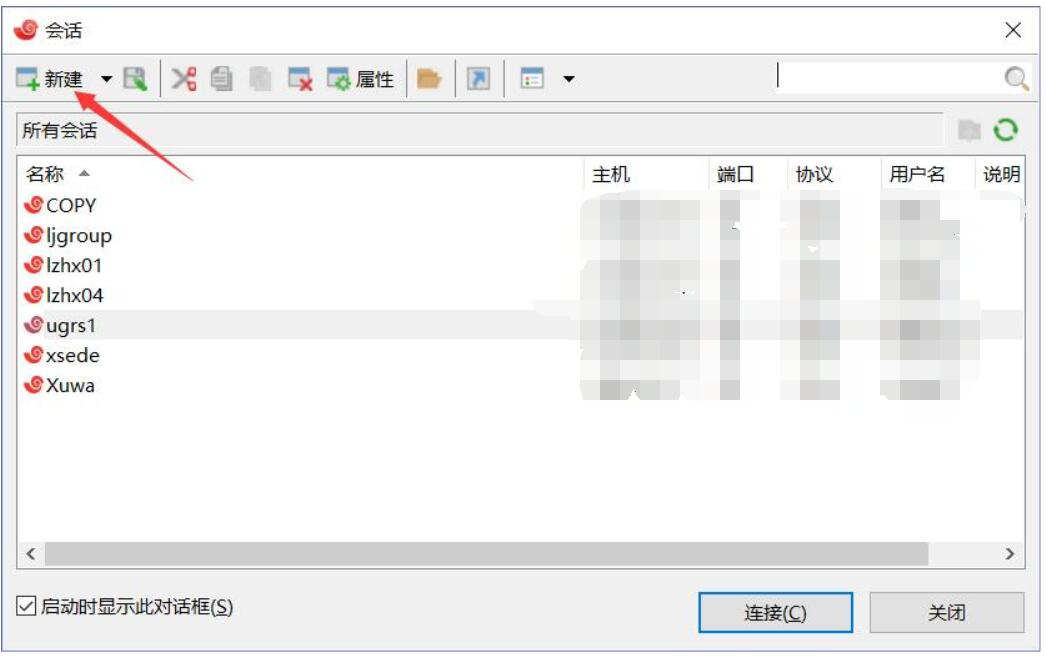
\includegraphics[width = 10cm]{fig/xshell1.jpg}
        \label{XSHELL6打开}
      }
      \subfigure[\textbf{\small{XShell6新建会话窗口}}]
      {
        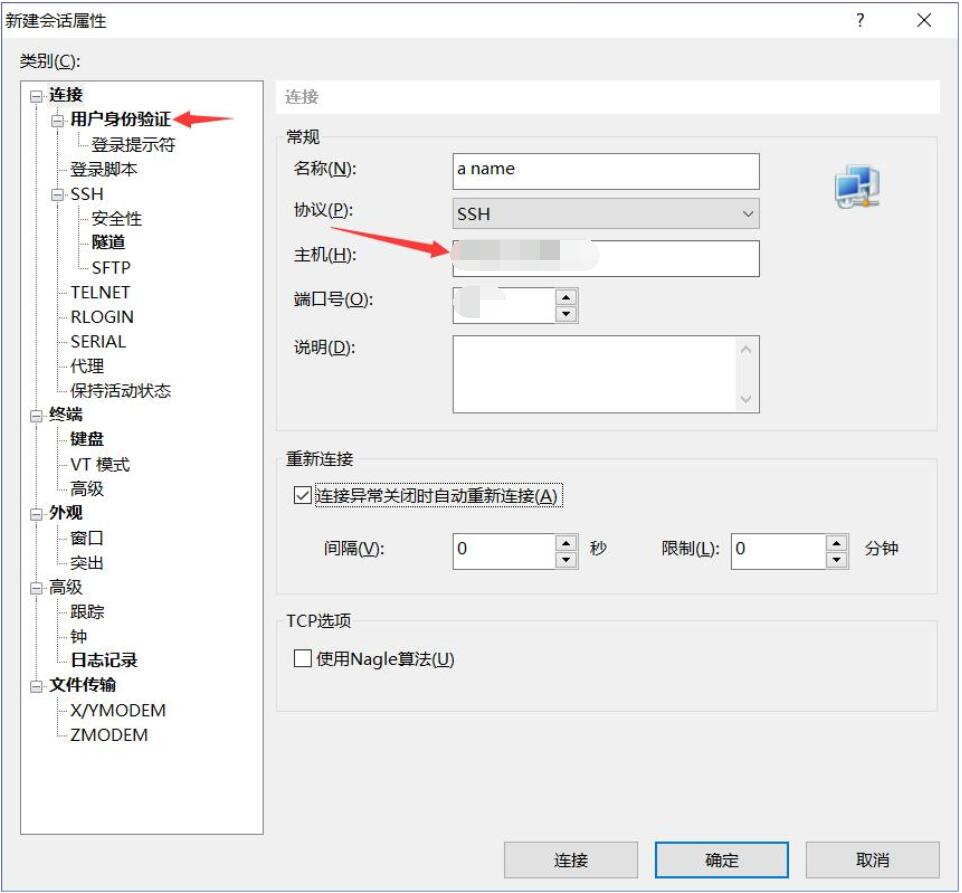
\includegraphics[width = 8cm]{fig/xshell2.jpg}
        \label{XSHELL6新建}
      }
      \caption{\textbf{XShell连接服务器}}
      \label{Xshell}
    \end{figure}
    
    随便起个名字,对应的主机,端口号,用户名,密码请向编者询问\footnote{我们有一个专为入门本科生注册的账号,主要供学习使用,毕设或者读研读博正式在组内工作会有新的账号},(注意:想要成功连接该IP需要浙大内网:ZJUWLAN、有线网络或者RVPN均可)。如果在输入账号密码登录之后见到类似Figure \ref{登录服务器}的界面,就代表已经成功登陆进我们的服务器,并处于\textbf{主目录}(通常用波浪线~表示)下,在光标左侧显示的内容即当前处于ugrs1\_LJ账号下(这个是编者的账号),登录在tc6000节点(主节点,或称登录节点)。
    \begin{figure}
      \centering
      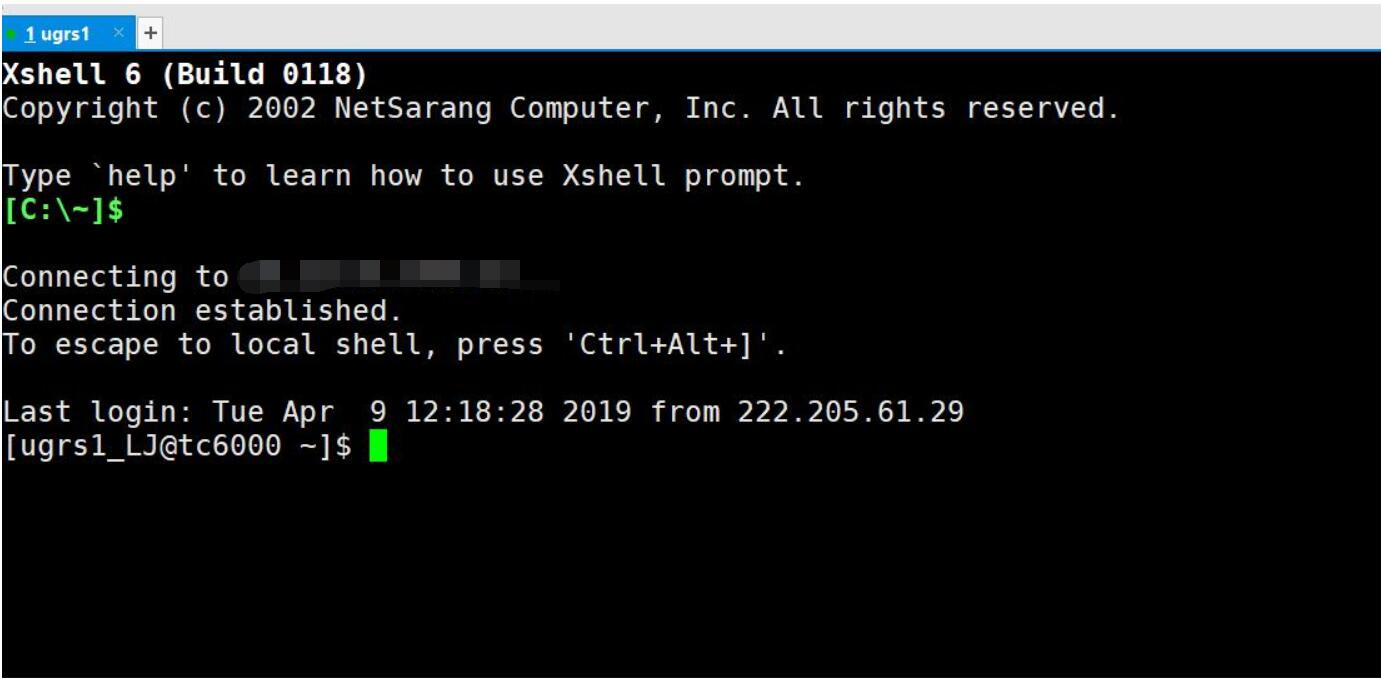
\includegraphics[width = 10cm]{fig/xshell3.jpg}
      \caption{\textbf{成功登陆服务器}}
      \label{登录服务器}
    \end{figure}
    
    登录服务器之后,就可以按照下一小节的内容进行操作,学习Linux系统的各类指令,和如何在Linux系统下编辑文件,为了安全起见,我们建议每个读者在主目录建立自己的文件夹,然后再自己的文件夹中进行各种操作,避免对他人的文件误操作而造成损失。

    \section{Linux基本操作}
    \begin{description}
    \item[cd]
      进入输入目录的文件夹;
      `cd folder/'
      P.S : `cd ..' 返回上一级文件夹
    \item[ls]
      列出所在文件夹的子文件夹;

    \item[vi / vim]
      打开文件查看内容;vim事实上是一个文本编辑器(比方说这个文档的一部分也是用vim编辑的),下面给出的只是vim常用指令,其实vim功能强大,需要其他操作时可自行查阅相关内容。

      P.S :输入不存在的文件可直接创立该文件;

    vim有一个梗,就是几乎所有的人刚上手的时候都不知道\textbf{该怎么退出}。在这里面稍微描述一下最基本的使用方法:
    \begin{description}
      \item[i / Ins] 如果已经打开了某个文本,那么这两个键中的一个能够允许你对文本作出修改。它左下角会显示 ``--INSERT--'' 这样的文段,这说明你处在编辑模式,这时候你按出的大部分操作会如同你使用大部分文本编辑器的时候一样,会完整地呈现在你正在修改的文本上。
  
      \item[Esc] 无论你处在何种模式,按了Esc你就能回到正常模式,在该模式下你可以用它自身的快捷键来直接作出一些修改,也可输入命令来完成别的操作(比如\textbf{退出})。

      \item[:q!] 这里`:'表示进行对vim程序自身的命令,`q'是quit,`!'表示强制。也就是输了这个命令并按回车后会强制退出并不保存文件。

      \item[:wq] 以此类推,这个表示的是保存并退出。没错,`:w'就是进行保存,并不退出。
      
      \item[:/xx] 向下搜索xx内容,按n转到下一个,N转到上一个。
      
      \item[:?xx] 向上搜索xx内容。  
      
      \item[:sp] 另外打开一个文件,可以使用Ctrl + W按两次的方式在不同文件间切换。  
      
      在编辑模式之外也可以对文本进行操作,常见操作如下(vim指令区分大小写):
      \item[V] 按行选取内容。
      \item[v] 按块选取内容。
      \item[Y] 复制选中内容。
      \item[P] 粘贴复制的内容\footnote{注意:vim里的复制粘贴是仅限在vim编辑器内使用的,而且和系统的复制粘贴(如Xshell提供的)独立}。
      \item[D 或 delete] 剪切选中内容,通常用作删除。
      \item[dd] 剪切当前行,通常用作删除。
    \end{description}
    好了,现在你也是会用vim的人了\footnote{在服务器输vimtutor回车有惊喜!}!跟我一起喊,\sout{vim天下第一!}
    \item[pwd]
      显示所在目录路径;它会显示所处目录的绝对路径,而这个绝对路径是你在任何别的目录下都能访问的。从该角度出发,事实上别的几乎所有操作都可以指定绝对路径(比如简单的访问,或者复制,或者在程序里面调用/生成文件)。

    \item[mkdir]
      在所在目录下建立文件夹:
      `mkdir levest' 表示建立名字为`levest'的文件夹

    \item[cp] 复制文件/文件夹至某个目录
      `cp einfield.com slot' 表示将`einfield.com' 在`slot'文件夹下进行粘贴,如果不存在这个文件夹,则在当前目录下生成一个名为'slot'的复制

    \item[mv] 原则上它表示将某个东西移动到什么地方,但它的另一个神奇操作在于它可以重命名文件/文件夹(后缀还是要加好)。

    \item[rm] \textbf{ 危险!}这是表示删除操作。
    
    \item[man] Linux帮助指令,比如使用man ls可以查看ls指令的全部功能。

    \item[-r] 在Linux中大部分的`-*' 表示了所进行的主要命令的附加指令(附加属性,\sout{buff})。像这里`-r'一般用来表示是对整个文件夹进行操作,像上面的cp, rm 都可以加上-r,但是mv指令比较特殊,mv对文件夹操作不需要-r。

    \item[*] *一般在Linux表示缺省符号,也就是在这里面可以填任何东西。比方说,`rm *.c' 表示任何后缀为`.c'的文件都会被删除\footnote{这就是为什么sudo rm -rf /* 这个梗会流行的原因,务必不要尝试。}。

    \end{description}

    读者可以在登录之后所在的主目录下先输入ls指令然后回车,看到当前目录下的文件和文件夹,然后输入“mkdir 文件夹名”的方式创建属于自己的文件夹,然后cd自己的文件夹,之后再这个目录下进行后续的操作。
    
    \section{使用服务器递交任务}
    我们的超算集群,简单地说是由很多的CPU(\textbf{节点})构成的,每个CPU有28个\textbf{核},据说服务器的单核运行效率其实是低于正常个人计算机的,但是优势在计算资源非常多。西溪校区的超算集群主要是王林军老师和洪鑫老师出资,也主要是这两个课题组在使用。王老师占有其中的48个节点,共1344个核。这些节点按照一定的顺序组合成了两个\textbf{队列},分别为ljcluster和ljtest,前者又可以分为wenchang和quantum,使用ljclustat指令可以看到全组的节点使用情况。尽管是为本科生学习练习使用的账号,ugrs3\_LJ账号仍然有对服务器三个节点的访问权限(即ljtest队列)。我们在服务器上递交任务,就是将自己的程序交给这些核去运算,要实现这个靠的是PBS任务管理系统。
    
    计算集群是由多台高性能服务器节点组成的,需要有一套系统能够为我们的计算任务自动分配资源,当计算资源出错的时候,能够避免将任务分到异常节点上去,当计算资源全部用完的时候我们再提交任务,能够有一个排队机制当之前的计算任务完成后自动将排处于队状态的作业自动运行。这就是PBS作业调度系统的主要作用。一个常见的PBS任务脚本如下图所示
    \begin{lstlisting}
      #PBS -N 2butene_PBE_0
      #PBS -l nodes=1:ppn=28
      #PBS -q ljcluster
      #PBS -l walltime=99:60:00
      #PBS -j oe
      nprocs=`cat $PBS_NODEFILE | wc -l`
      
      cd $PBS_O_WORKDIR
      cat $PBS_NODEFILE >> NODEFILE
      source /public/software/profile.d/mpi_openmpi-2.0.0-gnu.sh
      source /public/software/compiler/intel2017/mkl/bin/mklvars.sh intel64
      
      python nac.py > nac.out
    \end{lstlisting}

    这是一个调用PBS管理系统的脚本文件,里面的每一行都有其对应的意思,前几行以\#PBS开头的句子为PBS的调度信息相关的指令,-N 代表作业名,这个脚本的作业名为2butene\_PBE\_0,-l 为计算分配资源,图中为分配了一个节点,28个核,注意到第四行也是这类,分配了这个任务的最大运行时间为99小时60分钟(100小时),-q 代表使用哪个队列,图中即为使用ljtest队列,-j 的一行代表将标准输出信息(o)错误信息(e)合并输出到文件。接下来是bash命令行指令,第一行内容为获取本任务所调用的核数,并将这个数赋值给nprocs(在此脚本中此行为多余的,后面并没有用到nprocs),接下来的两行为打开PBS所在目录(也可以使用绝对目录)和将任务占用的节点信息输出到NODEFILE这个文件中,下面两行为环境变量设置,正常情况下不同任务的环境变量设置是不同的,需要根据任务对应的程序而修改,最后一行为执行命令(python)。需要注意,白色的部分为普通的bash脚本,因此可以根据需要任意添加。

    写完PBS文件之后(本例子中文件名即为PBS,可以按需修改),只需要执行“qsub PBS”指令就可以将这个脚本递交给PBS系统,而PBS系统负责根据这个脚本的内容为你分配计算资源,进行计算。希望查看自己的任务,可以使用“qstat”指令,可以打出所有正在服务器运行的任务,希望检索特定队列可以用“-a”,希望进行搜索可以在指令后添加额外的grep指令,举例:如果你希望输出所有在ljtest队列上运行的信息带有ugrs3的任务,指令是“qstat -a ljtest |grep ugrs3”。所有任务的后面会有一个status,R代表正在运行,Q代表正在排队等待运行,C代表运行完成(不代表算对,有可能是由于错误退出),E代表错误退出,H代表被挂起,H的任务即使排队到了资源也不进行计算,先让他之后的任务计算。

    此外,PBS系统还有诸多指令(如常用的qdel和qhold等),诸多功能,诸多环境变量可以调用,鉴于递交任务实际操作的重要性,这里不再赘述,如果在实际操作过程中希望有更多了解,可以参阅浙江大学西溪校区化学系HPC超算平台介绍(可在超算QQ群的群文件中找到)中的Gridview PBS作业调度使用说明。
    
    \chapter{数学基础}

    本章包含了在王老师课题组可能用到的数学知识,但是并不是所有人所有方向都非常重要,如果对线性代数基础知识和量子力学基础比较熟悉,可以有用到相关知识的时候再回来检索查看,如果不熟悉,还是建议阅读本章内容。当然,本指南不适合完全没学过线性代数的同学,如果想完整学习线性代数请参阅相关教材。

    \section{简易数学回顾}
    
    数学基础的第一小节将关注于最基础的数学内容,主要是线性代数和微积分的一些知识,由于长时间不用可能有所生疏,我们就在这里作简单的回顾。熟悉此节内容的同学可以直接跳过。

    \subsection{线性空间,线性映射与矩阵}

    对于矢量空间的数学定义,我们不做仔细讨论,简单地说,我们在某个数域$F$上定义了一个非空集合$V$,这个$V$中的元素满足加法交换律,对于数乘运算满足结合律,分配律等,而且数乘和加法的运算关于集合$V$是封闭的,我们就称$V$是一个线性空间,或者矢量空间,矢量空间内的元素称为矢量/向量。我们按照定义证明物理中的三维空间矢量是实数域上定义的线性空间,另外我们可以在矢量空间中定义内积和两个矢量的夹角,普适定义不再展开,本指南中将用最朴素的内积和矢量夹角定义方式,在三维下就是我们熟知的矢量模和夹角形式。

    对于线性空间中的向量,我们可以做线性组合,对于线性空间中的元素$\left\{\mathbf{a}_1,\mathbf{a}_2,\mathbf{a}_3,\dots,\mathbf{a}_N\right\}$,如果存在不全为零的系数$\left\{\lambda_i\right\}$使得
    \begin{equation}
      \lambda_1\mathbf{a}_1+\lambda_2\mathbf{a}_2+\cdots+\lambda_N\mathbf{a}_N=\mathbf{0}
    \end{equation}
    则称这个矢量组$\left\{\mathbf{a}_1,\mathbf{a}_2,\mathbf{a}_3,\dots,\mathbf{a}_N\right\}$的元素线性相关,否则称为线性无关。线性相关的向量意味着其中一个可以用其他向量的线性组合表示,也就是他们并不是独立的。在一个线性空间中可以找到的最大的线性无关向量组的个数称为这个线性空间的维度,比如在三维空间内我们最多可以找到三个线性无关的矢量,通常选用三个单位正交矢量。需要注意,线性无关不代表正交,二维空间内夹角为1度的两个矢量也是线性无关的\footnote{但是总可以通过Gram-Schmidt正交化或者其他正交化方法从一组线性无关的矢量构建同样个数的正交矢量}。这个最大的线性无关矢量组,就可以作为这个空间的基矢量,线性空间中的任何一个矢量都可以写成基矢量的线性组合。
    
    这个线性组合的系数通常是我们所关心的东西,在一组基矢量$\left\{\vec{e}_i\right\}$下,这个线性空间的任何向量都可以表示为
    \begin{equation}
      \vec{f}=\sum_i{N}c_i\vec{e}_i
    \end{equation}
    在定义了基矢量之后,我们没有必要每次都把基矢量写出来,因为一组完备的系数组就足够描述这个矢量。我们通常用一个含有N个(空间维度)元素的数组来表示一个矢量,比如说三维空间中的$(c_1,c_2,c_3)$。在这之后,我们可以定义一种映射$\mathcal{O}$,它把线性空间$V_1$内的元素映射到另一个线性空间$V_2$下,并且满足线性性,即
    \begin{equation}
      \mathcal{O}(\lambda\mathbf{a}+\mu\mathbf{b})=\lambda\mathcal{O}(\mathbf{a})+ \mu\mathcal{O}(\mathbf{b})
    \end{equation}
    则称$\mathcal{O}$是从$V_1$到$V_2$的线性映射,如果$\mathcal{O}$是把一个矢量映射到自己的线性空间,则也称为线性变换。我们知道,如果这个映射对于矢量空间的基矢量定义好了,所有矢量的映射就都定义好了。我们对基矢量中的$\vec{e}_i$做线性变换,由于其仍然位于这个线性空间下,所以变换完的矢量$\mathcal{O}(\vec{e}_i)$可以写成所有基矢量的线性组合:
    \begin{equation}
      \mathcal{O}(\vec{e}_i)=\sum_j^N  O_{ij}  \vec{e}_j 
    \end{equation}
    式中的$O_{ij}$可以认为是一个矩阵的矩阵元,这样一个线性变换就和一个矩阵一一对应\footnote{线性变换对应方矩阵,线性映射对应全部矩阵},而这个映射的逆映射也就与这个矩阵的逆矩阵相对应。同样的,对于一个矩阵
    \begin{equation}
      \mathbf{A}=\left( \begin{array}{cccc}{A_{11}} & {A_{12}} & {\cdots} & {A_{1 M}} \\ {A_{21}} & {A_{22}} & {\cdots} & {A_{2 M}} \\ {\vdots} & {\vdots} & { } & {\vdots} \\ {A_{N 1}} & {A_{N 2}} & {\cdots} & {A_{N M}}\end{array}\right)
    \end{equation}
    都对应着一个线性映射,对于一个写成列向量的$M$维矢量
    \begin{equation}
      \mathbf{a}=\left( \begin{array}{c}{a_{1}} \\ {a_{2}} \\ {\vdots} \\ {a_{M}}\end{array}\right)
      \label{column vector}
    \end{equation}
    矩阵$\mathbf{A}$可以将其转化为一个$N$维矢量$\mathbf{b}$
    \begin{equation}
      \begin{aligned}
        \mathbf{A} \mathbf{a}&=\mathbf{b}\\
        b_{i}=\sum_{j=1}^{M} A_{i j} a_{j} &\quad i=1,2, \ldots, N
      \end{aligned}
      \label{linear transformation}
    \end{equation}

    有一种线性变换,它满足在变换前后矢量的模长不变,这个性质保证了原本正交归一的基矢量在变换后是另一组正交归一的基矢量,这个性质在量子力学的表象变换中至关重要,这类变换称为正交变换,正交变换对应的矩阵为正交(orthogonal)矩阵,即满足
    \begin{equation}
      \mathbf{A}\mathbf{A}^{\mathsf{T}}=\mathbf{I}
    \end{equation}
    其中$\mathsf{T}$为转置符号,$\mathbf{I}$为单位矩阵,容易证明,满足这样条件的矩阵对应的线性变换是保持矢量模长的。

    \subsection{行列式}
    行列式在线性代数的书中有多种等价定义,为了与讲解量子化学推导内容的一致性,我们选用排列法的定义,即对于一个方矩阵
    \begin{equation}
      \operatorname{det}(\mathbf{A})=|\mathbf{A}|=\left| \begin{array}{ccc}{A_{11}} & {\cdots} & {A_{1 N}} \\ {\vdots} & {} & {\vdots} \\ {A_{N 1}} & {\cdots} & {A_{N N}}\end{array}\right|=\sum_{i=1}^{N !}(-1)^{p_{i}} \mathscr{P}_{i} A_{1i_1} A_{2i_2} \cdots A_{N i_N}
      \label{determinants defination}
    \end{equation}
    其中$\mathscr{P}_i$是排列算符,它的意义是给出一种列指标$1,2,3,\dots,N$的排列,求和就是关于所有的$N!$种排列求和,$p_i$是从自然序排列(1,2,3,\dots,N)出发得到排列$\mathscr{P}_i$所需要的近邻交换操作的个数。看似非常复杂,让我们以$3\times3$矩阵为例说明这个操作是如何实现的。

    对于$3\times3$矩阵的矩阵元乘积$A_{1i_1} A_{2i_2}A_{3i_3}$的排列总有$3!=6$种,即$i_1,i_2,i_3$分别等于$1,2,3$,$1,3,2$,$2,3,1$,$2,1,3$,$3,1,2$和$3,2,1$,接下来就是计算每种排列对应的$p_i$,即从$1,2,3$实现该排列所需要的近邻交换操作的个数,分别是$0,1,2,1,2,3$\footnote{你可能算出来跟我差一个偶数,但根据式(\ref{determinants defination})这不重要},所以$3\times3$矩阵的行列式计算表达式为
    \begin{equation}
      \operatorname{det}(\mathbf{A})=A_{11} A_{22}A_{33}-A_{11} A_{23}A_{32}+A_{12} A_{23}A_{31}-A_{12} A_{21}A_{33}+A_{12} A_{21}A_{32}-A_{13} A_{22}A_{31}
    \end{equation}
    可以看到与用Laplace展开定义的结果一致。

    矩阵的行列式最重要的一些性质有:如果矩阵不满秩(这个矩阵的每一列或者每一行单独写成一个向量,他们线性相关),矩阵的行列式为0,矩阵就没有对应的逆矩阵\footnote{矩阵有逆矩阵,等价于行列式不为0,没有逆矩阵的矩阵对应的线性映射也是不可逆的(损失信息)};$|\mathbf{A B}|=|\mathbf{A}||\mathbf{B}|$;任意交换行列式中的两列(行),矩阵行列式反号。

    \subsection{特征值与特征向量}
    在线性代数课程中,特征值与特征向量可能不被特别重视,\sout{当然主要原因是需要重视的东西太多了,}但是在物理学、工程的诸多应用中,特征值与特征向量几乎是整个线性代数最常用的一块知识点。

    线性代数中定义,如果矩阵$\mathbf{A}$右乘一个向量$\mathbf{X}$恒等于一个数$\lambda$乘以这个向量
    \begin{equation}
      \mathbf{AX}=\lambda\mathbf{X}
      \label{eigen defination}
    \end{equation}
    那么向量$\mathbf{X}$称为矩阵$\mathbf{A}$的对应特征值$\lambda$特征向量。如何求解特征值和特征向量其实非常简单,先假设特征向量存在,就有
    \begin{equation}
      \mathbf{AX}-\lambda\mathbf{I}\mathbf{X}=(\mathbf{A}-\lambda\mathbf{I})\mathbf{X}=0
      \label{eigen defination2}
    \end{equation}
    当$\mathbf{X}$不是零向量时,要求左边乘以它的矩阵的行列式为0,由此得到
    \begin{equation}
      \operatorname{det}(\mathbf{A}-\lambda\mathbf{I})=0
      \label{eigen equ}
    \end{equation}
    就可以求出特征值,将特征值代入(\ref{eigen defination})或(\ref{eigen defination2})就可以求出对应的特征矢量。其实可以看到一个特征值对应的特征矢量构成了一个线性空间,称为特征子空间。

    在应用中,我们经常需要将一个矩阵对角化,即通过线性变换使得矩阵变成对角阵,对角化通常是使用特征值与特征向量的方法。如果$n\times n$矩阵$\mathbf{A}$有n个特征值,对应n个特征向量,\sout{物理里的矩阵性质都很好的,}首先求出矩阵对应的特征值和(模为1)特征向量,将这些特征向量按列向量的形式组合成一个矩阵
    \begin{equation*}
      \mathbf{S}\equiv\left[ \begin{array}{lll}{x_{1}} & {\cdots} & {x_{n}}\end{array}\right]
    \end{equation*}
    计算矩阵$\mathbf{A}$乘以$\mathbf{S}$
    \begin{equation}
      \begin{aligned}
        \mathbf{A S}=\mathbf{A} \left[ \begin{array}{ccc}{x_{1}} & {\dots} & {x_{n}}\end{array}\right]=\left[ \begin{array}{lll}{\lambda_{1} x_{1}} & {\cdots} & {\lambda_{n} x_{n}}\end{array}\right]=\\ \left[ \begin{array}{ccc}{x_{1}} & {\dots} & {x_{n}}\end{array}\right] \left[ \begin{array}{ccc}{\lambda_{1}} & { } & { } \\ { } & {\ddots} & { } \\ { } & { } & {\lambda_{n}}\end{array}\right]=\mathbf{S }\Lambda
      \end{aligned}
    \end{equation}
    其中$\Lambda$是由矩阵$\mathbf{A}$的n个特征值构成的对角矩阵,所以我们得到
    \begin{equation}
      \mathbf{S^{-1}AS}=\Lambda
    \end{equation}
    这就得到了一个对角阵。

    什么样的矩阵可以对角化是一个很复杂的问题,我们只给出一个充分条件,实对称矩阵(矩阵和它的转置相等)一定可以在实数范围内对角化得到实数特征值,并且不同特征值对应的特征矢量是正交的。而与之相反的是反对称矩阵(矩阵和它的转置相差负号),反对称矩阵在实数范围内无法对角化。
    
    \subsection{向复数域推广}
    接下来做推广,上述矢量空间均为定义在实数域上的,可以不做任何额外修正,完全转化到复数域,矩阵元,向量的分量,都可以为复数。在这个意义下,我们习惯将一个矢量写成列矢量的形式,就像式(\ref{column vector})那样。我们定义矩阵和向量的共轭转置,用$\dagger$符号表示
    \begin{equation}
      \begin{aligned}
        \left(\mathbf{A}^{\dagger}\right)_{i j}=A_{j i}^{*}\\
        \mathbf{a}^{\dagger}=\left(a_{1}^{*} a_{2}^{*} \cdots a_{{M}}^{*}\right)
      \end{aligned}
    \end{equation}
    在复数域的线性空间内,矢量的内积定义为行矢量和列矢量的乘积
    \begin{equation}
      \mathbf{a}^{\dagger} \mathbf{b}=\left(a_{1}^{*} a_{2}^{*} \cdots a_{{M}}^{*}\right) \left( \begin{array}{c}{b_{1}} \\ {b_{2}} \\ {\vdots} \\ {b_{M}}\end{array}\right)=\sum_{i=1}^{M} a_{i}^{*} b_{i}
      \label{inner product in row and column }
    \end{equation}
    可以看到,$\mathbf{a}=\mathbf{b}$时,我们可以定义的矢量模平方,在复数域上刚刚好是矢量每个元素的模的平方和。在复数域下,矩阵原本的很多性质都得到保持,只是简单地向复数域的推广,毕竟实数域是复数域的一部分,向更全的集合的推广往往能得到更加普适的性质。

    在复数域上有很多特殊的矩阵,比如幺正(unitary)矩阵\footnote{由于翻译问题部分教材称为酉矩阵},是正交矩阵的推广,满足
    \begin{equation}
      \mathbf{A}\mathbf{A}^{\dagger}=\mathbf{I}
      \label{unitary def}
    \end{equation}
    在复数域上保持矢量模不变的线性变换,对应的就是幺正矩阵。而实对称矩阵的推广就是厄米矩阵(自伴矩阵),厄米矩阵定义多种多样,我们取其中最简单的一种,即
    \begin{equation}
      \mathbf{A}=\mathbf{A}^{\dagger}
    \end{equation}
    可以看出,如果矩阵元都是实数,厄米矩阵就是实对称矩阵。厄米矩阵和实对称矩阵的性质相似:具有实数的特征值,并且不同特征值对应的特征向量正交。

    最后讨论一种特殊的矩阵,正规矩阵,定义为
    \begin{equation}
      \mathbf{A}\mathbf{A}^{\dagger}=\mathbf{A}^{\dagger}\mathbf{A}
    \end{equation}
    从这个定义看出,厄米矩阵和幺正矩阵都是正规矩阵。我们介绍在复数域上正规矩阵的谱定理,\sout{证明留作习题}
    \begin{theorem}
      设我们在复数域上定义线性空间$V(F),F=C$且$\mathbf{A}$是这个线性空间的一个元素,则以下条件等价:\\
      1.$\mathbf{A}$是正规的;\\
      2.$V$有一个由$\mathbf{A}$的本征向量构成的正交归一基;\\
      3.$\mathbf{A}$在$V$的某个正交归一基下是对角矩阵。
    \end{theorem}

    \subsection{向函数空间推广}
    学完线性代数大家都知道,一个线性空间可以由一组基矢量来描述,我们生活的三维空间可以用三个相互正交的单位矢量做展开,看起来都是平凡的。但是线性空间的定义远远不限于通常的“矢量”的空间,你学完现代的时候可能并不会意识到函数空间其实也是线性空间。

    以最简单的多项式为例,首先我们写成一个任意的n阶多项式
    \begin{equation}
      P_n(x)=\sum_{i=0}^n c_i x^i
    \end{equation}
    可以看到,它也是由n个小函数$\left\{1,x,x^2,x^3,\dots,x^n\right\}$线性组合成的,而且如果这个多项式恒等于0的话,我们必须要求每一个系数$c_i$都等于0,如果回忆一下线性无关的定义,我们就会发现这几个函数其实是线性无关的,而且这n个函数已经能表示出任意一个n阶多项式,你可以回顾线性空间的定义,n阶多项式的集合其实是一个n维线性空间,就可以选用$\left\{1,x,x^2,x^3,\dots,x^n\right\}$作为这个线性空间的一个基。

    那么这组基矢量是否正交呢,这就涉及到一个复杂的问题,函数的内积怎么定义,我们上文中其实没有展开内积的定义,我们此处也不深究。矢量的内积通常为对应系数乘积求和,函数的内积通常定义为在某个空间内,两个函数乘积的积分,即
    \begin{equation}
      \left(f,g\right)=\int_a^b dx f(x)\times g(x)
    \end{equation}
    如果这两个函数是复函数,上式的定义中通常将$f(x)$换为它的复共轭$f^*(x)$,如果取积分是从$-1$到$1$,可以看到上面我给出的这组基是不正交的(当然这不影响他们线性无关)。接下来,我们做一个不那么平凡的推广,那就是任意多项式的集合也是一个线性空间,维数为无穷\footnote{从有限到无穷的推广通常不能这么随意},有无穷多个函数构成的基矢量组,我们也可以用类似Gram-Schmidt 正交化的方法来定义一组正交基,读者如果有兴趣,可以从我们给出的这组基出发,做Gram-Schmidt 正交化,就会得到勒让德多项式(会相差一个系数,但是系数不影响正交性)。

    同样,很多函数空间,比如全体平方可积函数(函数平方在全空间积分为有限值)的集合,全体连续函数的集合,全体一阶导连续函数的集合等等,都可以构成一个线性空间,当然它们都是无穷维的。我们常见的基函数也有很多种,比如上面提到的勒让德多项式,它虽然复杂,但只是一组多项式而已,如果大家的微积分学的不错,应该会想到,傅里叶级数其实就是把函数在三角函数基上展开,并且求解这个展开系数。
    
    波函数通常被说成是一个希尔伯特空间\footnote{编者并不是很确定这个线性空间的严格数学定义,物理上通常就说平方可积的函数的集合是希尔伯特空间}的态矢量,所以有时候它写成函数,有时候又可以用矩阵力学的语言写成一个向量,而最终就会发现,它们是等价的。
    
    \section{符号使用}
    在量子力学相关领域,人们使用``左矢''(bra)和``右矢''(ket)来描述一个``状态''。我们可以先简单地认为右矢代表了一个列向量,左矢则代表了一个行向量。它们是这么表示的:
    \[
    | \xi \rangle \rightarrow \text{右矢}, \langle \xi | \rightarrow \text{左矢}    
    .\]  
    我们知道,一个行向量和列向量相乘能够得到一个实数,这也可以理解为两个行向量进行内积的过程,比如两个右矢$| \xi_1 \rangle $ 和$| \xi_2 \rangle $ ,此时它表示为
    \[
    \langle \xi_1 | \xi_2 \rangle 
    .\] 
    当然量子力学远不止于此,它有可能包括了各种奇奇怪怪的东西,使得它并不能完全用向量来描述,比如在线性代数里我们有时候需要用矩阵,在量子力学里它们统统被概括为算符。算符是作用在矢量上的。如果你学过张量分析/矢量代数,你还可以认为它代表了一个张量。有些人们喜欢用$\hat{Q}$类似这样的形式来表达一个算符(也就是加个帽子),也有些人喜欢用粗体,比如$\mathbf{Q}$这样来表达,也有人不加任何东西\footnote{没错就是发明这一套符号系统的\Large{Dirac}大佬。},只要它``在该在的地方''就可以识别为一个算符。算符放在左矢的右边,或者右矢的左边,或者左矢和右矢的中间,也就是
    \[
    \hat{Q}| \xi \rangle ,\langle \xi | \hat{Q}, \langle \xi_1 | \hat{Q} | \xi_2 \rangle   
    .\] 
    到了这里,当然就会出现作用顺序(方向)的问题。不过其实这一套和线性代数非常相像\footnote{事实上这一套就是线性代数——也就是海森堡开发的矩阵力学的核心,量子力学就是线性代数(并不是)},算符默认是作用在右边的,如果需要作用在左矢,那么对应的算符为原算符的厄米共轭(Hermite Conjugate),用$\hat{Q}^\dagger$来表达。那么某种程度上,左矢代表的是右矢的共轭转置,左矢和右矢相作用得到的是两者的内积。

    当然这么说可能很难有感觉这些到底是什么东西,让我们再换一种方式来表达。算符,变换,这些东西实则上都代表了类似于函数的概念,也就是传进去一个东西,传出去另一个东西,这两个东西可以相等,可以完全不是同一类。而左矢和右矢则代表了可以传进去的``参量'',并经过算符作用后得到了另一个左矢或右矢。比如一个关于$x$的函数$f(x)$,经过求导算符$\frac{d }{d x} $作用后得到它的导函数$f'(x)$,实则上也没有脱离这样的描述体系\footnote{从而为Dirac说明海森堡的矩阵力学和薛定谔的波动力学是等价表述做好了铺垫。}。

    \section{简易矢量代数}
    鉴于量子力学推导中会出现$\nabla$符号,与之相关的梯度,散度,旋度的概念在物理学中有极为重要的意义,更是广泛出现在各类推导之中,本节将介绍这三个“度”的定义和与之相关的Green公式和Stokes公式。

    如果有一个一元函数$f(x)$,那么这个函数的微分可以写成
    \begin{equation}
      \mathrm{d} f = \frac{\mathrm{d} f}{\mathrm{d} x} \mathrm{d}x
    \end{equation}
    它的意义明确,当$x$改变$ \mathrm{d}x $时,函数值将改变$ \mathrm{d}f $,两者之间的商就是微商(导数)。但是如果函数是多个变量的呢?比如说我们在空间中有一个温度分布$T(x,y,z)$,如果我们希望描述这个函数随着空间变化的变化量时,我们必须先指定是往空间的哪个方向变化,这样看起来就变得复杂了很多,但是我们仍然有
    \begin{equation}
      \mathrm{d}T = \frac{\partial T}{\partial x}\mathrm{d}x  +\frac{\partial T}{\partial y}\mathrm{d}y+\frac{\partial T}{\partial z}\mathrm{d}z
    \end{equation}
    上式其实还可以写成矢量点积的形式
    \begin{equation}
      \mathrm{d}T = (\frac{\partial T}{\partial x},\frac{\partial T}{\partial y},\frac{\partial T}{\partial z})\cdot(\mathrm{d}x, \mathrm{d}y, \mathrm{d}z)
    \end{equation}

    \section{简易数值计算方法}
    我们一般将可以直接写出数学表达式的问题称为解析的,与之对应的就是数值的。虽然解析的数学在相当多的方面都有重要意义,但是对于实际的应用来说,尤其是计算机模拟的问题来说,得到解析表达式是极为困难。举个简单的例子,常微分方程,就连本科生课程中给出的例子很多都需要做数值计算才能真正得到结果。而在王老师课题组,由于研究的都是动力学问题,即体系随时间演化,更是需要很多数值拟合,微分积分和数值解微分方程的概念,因此本节中我们将极其简要地介绍相关问题的最基础方法,实际操作中需要较高精度方法请参阅相关书籍。
    \subsection{插值与拟合}
    \subsection{数值微分和数值积分}
    \subsection{ODE初值问题的数值解法}

    \section{完备基展开}
    完备基展开是一个非常重要的概念,它直接提供了解决众多微分方程的方法,而解决微分方程是量子力学的至关重要的一个内容。

    ``完备''一词说明某一个基组的完备性,也就是我只要通过这个基组的线性组合就能完整描述我所研究的空间中的所有向量。我用$\hat{x}$,$\hat{y}$,$\hat{z}$三个基向量就能完整描述三维空间里的所有向量,我用${x^n}$便能描述一维的所有函数,我用${\sin{nx},\cos{nx}}$就能描述有限空间内的函数/周期性函数,这些都构成了所谓的完备基。

    在这里请允许编者引入施图姆-刘维尔型方程和对应本征值问题。
    \begin{theorem}
    	对形如
	\begin{equation}
		\frac{d }{d x} \left[ k(x) \frac{d y}{d x}  \right] -q(x)y + \lambda \rho(x) y = 0 \quad (a\leqslant x \leqslant b)
	\end{equation}
	的方程,若$k(x),k'(x),q(x)$ 连续或最多以$x=a$ 和$x=b$ 为一阶极点\footnote{也就是最低项为$\frac{1}{x}$ 项。},则
	\begin{enumerate}
		\item 存在无穷多个本征值
		\[
		\lambda_1 \leqslant \lambda_2 \leqslant \lambda_3 \leqslant ...
		,\] 
		相应地有无限多个本征函数
		\[
			y_1(x),y_2(x),y_3(x),...
		.\] 
		这些本征函数的排列持续正好使节点个数依次增多(即函数值为零的点的个数)。
		\item 所有本征值 $\lambda_n \geqslant 0$,
		\item 相应于不同本征值$\lambda_m$ 和 $\lambda_n$的本征函数$y_m(x)$和$y_n(x)$在区间$[a,b]$上带权重$\rho(x)$正交,即
			\begin{equation}
				\int ^b_a y_m(x) y_n(x) \rho(x) \, dx = 0 
			\end{equation}
		\item 本征函数族$y_1(x),y_2(x),y_3(x)...$是完备的,即函数$f(x)$如具有连续一阶导数和分段连续二阶导数,且满足本征函数族所满足的边界条件,就可以展开为绝对且一致收敛的级数
			\[
				f(x) = \sum_n f_n y_n(x)
			.\] 
	\end{enumerate}
    \end{theorem}
    并由此引入广义傅里叶级数展开
    \[
	    \int ^b_a f(x) y_m(x) \, dx = \sum_n \int^b_a f_n y_m(x)y_n(x) \, dx = f_m \int^b_a y_m(x)^2 dx   
    .\] 
    即
    \[
	    f_m = \frac{\int ^b_a f(x) y_m(x) \, dx }{\int^b_a y_m(x)^2 \, dx }
    .\] 
    这一套系统非常的重要,它能够直接用来解决球坐标下的稳态问题(使用Legendre函数),柱坐标下的稳态问题和动态演化问题(使用贝塞尔函数),以及球坐标下的时间演化问题(使用球贝塞尔函数),其核心内容就在于使用广义傅立叶级数进行展开得到精确解并同时满足边界条件。

    没什么感觉?在这里举一个非常典型的例子,二维传热稳态问题,
    \begin{quote}
	    均匀的薄板占据区域$0<x<a,0<y<\infty$,边界上的温度
	    \[
		    u\big|_{x=0} = 0, u\big|_{x=a} = 0, u\big|_{y=0} = u_0, \lim_{y \to \infty} u =0
	    .\] 
	    求解板的稳定温度分布。
    \end{quote}
    传热这东西,它满足一个扩散方程
    \begin{equation}
	    \frac{\partial u}{\partial t} -a^2 (\frac{\partial ^2 u}{\partial x^2 } + \frac{\partial^2 u}{\partial y^2} + \frac{\partial ^2 u}{\partial z^2}  ) = 0.
    \end{equation}
    稳态,也就是它不随时间变化,$\frac{\partial u}{\partial t} = 0$,而这是二维,所以
    \begin{equation}
	    \frac{\partial ^2 u}{\partial x^2 } + \frac{\partial ^2 u}{\partial y^2 } = 0.
	    \label{2Ddiffusion}
    \end{equation}
    先分离变量,设$u=X(x)Y(y)$,代入(\ref{2Ddiffusion}),左右同除以$u$,
    \begin{equation}
	     \frac{d ^2 X}{X d x^2} = - \frac{d ^2 Y}{Y d y^2} = -k^2 .
    \end{equation}
    由于左边只关于$x$,右边只关于$y$,那么它们只能等于一个常数,考虑到在$x$方向上的边界条件(两边为零,不应该是指数型函数),它们应等于一个负数$-k^2$.
    直接解这个常微分方程,得到
    \begin{equation}
    	\begin{cases}
		X = A_k\sin{kx} + B_k\cos{kx} \\
		Y = C_k e^{-kt}
    	\end{cases}.
    \end{equation}
    由于这个世界实在不太可能有无穷大的温度,故$Y = e^{kt}$项不考虑。

    考虑到$u\big|_{x=0} = u\big|_{x=a} = 0$,$k$应该要满足某种条件才能满足这个,那么事实上
    \begin{equation}
	    X = A_n \sin{\frac{n\pi x}{a}} , k = \frac{n\pi x}{a}, n \in N_+.
    \end{equation}
    由于前面提到的本征值问题,$-k^2$是$X$的常微分方程的本征值,对应本征函数构成完备基,对$Y$也有相应情况,从而$u$可以展开为$XY$的线性组合,即
    \begin{equation}
	    X = \sum_n A_n \sin{\frac{n\pi x}{a}} e^{- \frac{n\pi y}{a}}.
    \end{equation}
    可是……$A_n$怎么确定呀?
    
    就是广义傅立叶级数呀!
    注意到$u\big|_{y=0} = u_0$,有
    \begin{equation}
	    A_n = \int ^a_0 u_0 \sin{\frac{n\pi x}{a}} \, dx = \frac{a u_0}{n\pi} (1-\cos{n\pi}) .
    \end{equation}
    于是我们成功地获得了温度分布的解析解!(?)\footnote{当然有些人会觉得级数展开不算解析解。能展开成简单函数求和已经不容易了。}

    花了这么多篇幅,只是想要说明完备基展开是一个非常重要的内容,它提供了一个解决复杂的微分方程问题的方法\footnote{其实线性代数里的本征值和本征向量也有同样的性质。}。同时它从某种角度上已经道明了量子力学的一个重要的点:
    \begin{center}
    	所有的态都能用本征态的线性组合来表示。
    \end{center}

    哦,我们的读者,然而故事还没有结束呢。

    我们先用曾经描述的量子力学符号来说说这个完备基。对于某个完备的特征值集$\{\lambda_n\}$和特征向量集$\{| e_i \rangle \}$,我们认为特征向量集已经正交归一\footnote{即不同的两个特征向量之间相互正交,且每个向量模为1(即\sout{自交}自己与自己的内积为1)。你可能还记得存在多重特征根的情况,此时你或许也记得这个特征根对应多个特征向量,它们并不一定需要正交。那么你想想就能明白,你能通过某些奇技淫巧让它们互相之间变得正交并仍旧是特征向量(比如大名鼎鼎的Gram-Schmidt 正交化)。},那么有定理
    \begin{theorem}
	\begin{equation}
		\sum \ket{e_i}\bra{e_i} = 1 \, / \, \int dq' \, \ket{q'}\bra{q'} = 1.
	\end{equation}
    \end{theorem}

    $| e_i \rangle \langle e_i | $是一个全新的操作,事实上它其实就是一个算符。为什么呢?因为你可以看到,
    \begin{equation}
      (| e_i \rangle \langle e_i | ) | \xi \rangle = | e_i \rangle \langle e_i | \xi \rangle = \langle e_i | \xi \rangle | e_i \rangle  .
      \label{ ket bra }
    \end{equation}
    这是由于$ \langle e_i | \xi \rangle $是一个数,所以它可以游荡在任何地方(向量可以非常自然地乘上任何一个数而不需要管顺序)。也就是我作用于$| \xi \rangle $然后获得了一个新的向量,那么它就是一个算符。

    $1$是沿用了Dirac大佬的写法\footnote{编者表示被Dirac虐得越多\sout{对Dirac越爱得深沉}},就是表示单位算符(或者单位矩阵),作用后得到原来的结果,即
    \begin{equation}
    	1 | \xi \rangle = | \xi \rangle .
    \end{equation}
    所以上面的定理就是在说我把特征向量按照那种方式组合求和后它就会变成单位算符。

    \begin{proof}
    	证明思路:验证其对完备基中任意向量都成立$\Rightarrow$空间内任意向量皆成立

\begin{equation}
	\sum_i \ket{e_i}\bracket{e_i}{e_j} = \sum_i\ket{e_i} \delta_{ij} = \ket{e_j}.
\end{equation}
从而说明该算符对所有特征向量都满足自身为单位算符。

利用展开的唯一性(即一个向量只有一种方式展开/系数组是唯一的),得到
\begin{equation}
\ket{\psi} = \sum c_i \ket{e_i} \Rightarrow c_i = \bracket{e_i}{\psi}.
\end{equation}
因此对所有向量皆满足自身为单位算符。
    \end{proof}
    恭喜你发现了\sout{镇站之宝},展开系数为
    \begin{equation}
      c_i = \langle e_i | \psi \rangle 
      \label{expansion coeff}
    \end{equation}
    是不是有那么一点感觉?其实就是广义傅立叶级数展开。

    oh忘记说了,$\delta_{ij}$这是(离散)狄拉克函数,它表示$i=j$时其值为1,$i\neq j$时为零。同样地,对于连续狄拉克函数$\delta(x)$,表示$x=0$时其值不为零(或者正无穷),$x\neq 0$时恒为零,同时保证
    \begin{equation}
	    \int \delta(x) \, dx = 1 
    \end{equation}
    它还有这些性质,
    \begin{align}
\delta(-x) & = \delta(x) \\
x\delta(x) & = 0 \\
\delta(a x) & = a^{-1} \delta(x)\\
\delta(x^2-a^2) & = \frac{1}{2} a^{-1} {\delta(x-a)+\delta(x+a)} \quad (a>0)\\
\int \delta(a-x) \, dx \, \delta(x-b) & = \delta(a-b) \\
f(x) \delta(x-a) &=  f(a)\delta(x-a)\\
\int f(x)x\delta(x) \, dx & = 0
\end{align}

    \section{傅立叶变换}
  \begin{quote}
    它,改变了世界。
    \begin{flushright}
      ——李睿,谈傅立叶变换时
    \end{flushright}
  \end{quote}     
  还记得傅立叶级数嘛?它长这样:
  \begin{theorem}
  当一个有界函数在$[-l,l]$可积时,该函数可展开为:
  \begin{equation}
    f(x) = \sum_k a_k \cos{\omega_k x} + b_k \sin{\omega_k x}.
  \end{equation}
  其中,
  \begin{equation} 
\begin{cases}
  a_k = \frac{1}{\delta_k l}\int _{-l} ^l f(\xi) \cos{\omega_k} \xi \, d\xi \\
  b_k =  \frac{1}{l} \int _{-l} ^l f(\xi) \sin{\omega_k \xi} \, d\xi 
\end{cases}
.
\end{equation}
其中
\begin{equation}
\omega_k = \frac{k \pi}{l}.
\end{equation}
以及
\begin{equation}
  \delta_k =
  \begin{cases}
  1, \quad k = 0 \\
  2, \quad k \neq 0 
  \end{cases}
  .
\end{equation}
 \end{theorem}

我们刚刚描述过完备基展开,而且$\sin{\frac{k \pi}{l} x}$和$\cos{\frac{k \pi}{l} x}$恰好是 $f''(x) + \lambda f(x) = 0$的解,所以它们在$[-l,l]$上构成了完备基,而且它们互相之间是正交的。在这里值得一提的是,$\sin{\frac{k \pi}{l} x}$满足了\textbf{第一类齐次边界条件},即在边界上函数值为零,而$\cos{\frac{k \pi}{l} x}$满足了\textbf{第二类齐次边界条件},即在边界上的一阶导为零,这允许我们在各类边界条件下研究一个物理问题。同时从某种意义上,我们可以说
\begin{center}
\textbf{边界条件导致了特征值的分立。}
\end{center}
比如在氢原子模型的解里,我们事实上引入了一些“自然边界条件”:在球坐标下的函数必须要满足
\begin{equation}
f(r,\theta, \phi) = f(r,\theta, \phi + 2\pi)
\end{equation}
这引发了角向的特征值分立,也就是\textbf{磁量子数的分立}。

而我们认为波函数在空间的任何一个点都是不发散的,因此在$\theta$方向上必须要展开成多项式而非无穷级数,而$\phi$方向的方程使它必须要符合连属Legendre多项式的形式\footnote{详细讨论还是见任何一本数学物理方法的书。}。同时波函数在全空间下是绝对可积的(因为我们已经定义了波函数的内积——它必须是在Hilbert空间下的),所以在无穷远处它必须收敛于零,这使得径向函数必须满足球Bessel函数的形式。所以从某种角度而言,\textbf{量子力学的能级分立是由于量子力学是使用一个偏微分方程描述且存在边界条件的}。

如果我们想要展开的是一个全实数域的函数呢?令$l \to \infty$,我们发现它转换为一个积分,
\begin{equation}
  f(x) = \int _0 ^\infty A(\omega) \cos{\omega x} \, d\omega + \int _0 ^\infty B(\omega) \sin{\omega x} \, dx  
.
\end{equation}
而系数为
\begin{equation}
\begin{cases}
  A(\omega) = \frac{1}{\pi} \int ^\infty _{-\infty} f(\xi) \cos{\omega \xi} \, d\xi \\
  B(\omega) = \frac{1}{\pi} \int ^\infty _{-\infty} f(\xi) \sin{\omega \xi}\, d\xi 
\end{cases}
.
\end{equation}

我们对它们进行改装,便转化为了复数域中的傅立叶变换以及对应的傅立叶逆变换,即
\begin{equation}
F(k) =  \mathcal{F} [f(x)] = \frac{1}{2\pi}\int_{-\infty}^{\infty} f(x) e^{-ikx} \, dx 
.
\end{equation}
以及
\begin{equation}
  \mathcal{F}^{-1} [F(k)] = \int_{-\infty} ^\infty F(k) e^{ikx} \, dk
\end{equation}
 这便是一般意义下的傅立叶变换\footnote{其实也有不少地方把那个系数$\frac{1}{2\pi}$分摊在正变换与逆变换上。}。我们从完备基上也可以理解,事实上傅立叶变换就是对$e^{-ikx}$进行展开,从而转化为频谱信息。

我们还能够引入各种定理,
\begin{theorem}
\begin{equation}
  \mathcal{F}[f'(x)] = ik F(k)
  \end{equation}
\end{theorem}
\begin{proof}
\begin{align*}
  \mathcal{F}[f'(x)] &=\frac{1}{2\pi}\int ^\infty_\infty f'(x) e^{-ik x} \, dx \\
         &= \frac{1}{2\pi}\left[ f(x) e^{-ik x} \right] ^\infty _{-\infty} - \frac{1}{2\pi}\int ^\infty _{-\infty} f(x) \left[ e^{-ik x} \right] ' \, dx 
\end{align*}
傅立叶变换要求原函数在整个空间上绝对可积,从而有$\lim_{x\to \pm \infty} f(x) = 0$,所以
\[
  \mathcal{F}[f'(x)] = - \frac{1}{2\pi}\int ^\infty_{-\infty} f(x) \left[ e^{-ik x} \right] '  \, dx = ik F(k) 
.\] 
\end{proof}
\begin{theorem}
\begin{equation}
  \mathcal{F}[f(x-x_0)] = e^{-ikx_0} F(k)
\end{equation}
\end{theorem}
\begin{proof}
  \[
    \mathcal{F}[f(x-x_0)] =\frac{1}{2\pi} e^{-ikx_0}\int ^\infty_{-infty} f(x-x_0) e^{-ik(x-x_0)} \, d(x-x_0) = e^{-ikx_0} F(k)
  .\] 
\end{proof}
\begin{theorem}
  \begin{equation}
    \mathcal{F}[f_1(x) * f_2(x)] = 2\pi F_1(k)F_2(k)
  \end{equation}
\end{theorem}
\begin{proof}
  \[
    \mathcal{F}[f_1*f_2] = \frac{1}{2\pi}\int ^\infty_{-\infty} \left[ \int ^\infty_{-\infty} f_1(\xi) f_2(x-\xi) \, d\xi   \right] e^{-ikx} \, dx 
  .\] 
  交换积分次序,
  \[
    \mathcal{F}[f_1*f_2] = \frac{1}{2\pi} \int ^\infty _{-\infty} f_1(\xi) \left( \int ^\infty_{-\infty} f_2(x-\xi) e^{-ik x} \, dx  \right) \, d\xi 
  .\] 
  利用延迟定理,
  \[
    \mathcal{F}[f_1 * f_2] = \frac{1}{2\pi} \int ^\infty_{-\infty} f_1(\xi) e^{-k\xi} \, d\xi \cdot 2\pi F_2(k) = 2\pi F_1(k)F_2(k)
  .\] 
\end{proof}

当然傅立叶变换不只是在一维上。我们对三维空间$\mathbf{r}$也可以做傅立叶变换,
\[
  F(\mathbf{k}) = \frac{1}{(2\pi)^{\frac{3}{2}}} \iiint f(\mathbf{r})  e^{-i\mathbf{k}\cdot\mathbf{r}  } \, d\mathbf{r} 
.\] 

傅立叶变换的一个非常有价值的特点是可以把导数转换为一个常数相乘,从而极大地简化方程。比如无界空间下的扩散问题,
\[
  u_t-a^2u_{xx} = 0
.\] 
初始条件:
\[
  u\big|_{t=0} = \phi(x)
.\] 
傅立叶变换再逆变换就能回到原来的样子,
\[
  u(x,t) = \int \mathcal{F}[u] e^{ikx} \, dk = \mathcal{F}^{-1}[\mathcal{F}[u]]
.\] 
对$x$做Fourier Transform,
\[
  \mathcal{F}[u](k,t) = \frac{1}{2\pi} \int u(x,t) e^{-ikx} \, dx 
.\] 
原方程便转换为
\[
\begin{cases}
  \mathcal{F}[u_t] + a^2 k^2 \mathcal{F}[u] = 0 \\
  \mathcal{F}[u]\big|_{t=0} = \mathcal{F}[\phi]
\end{cases}
.\] 
\[
  \Rightarrow \mathcal{F}[u] = \mathcal{F}[\phi] e^{-k^2 a^2 t}
.\] 
\[
  u = \mathcal{F}^{-1} [\mathcal{F}[\phi] e^{-k^2a^2 t}]
.\] 
有
\[
  \mathcal{F}[f_1 * f_2] = 2\pi \mathcal{F}[f_1] \mathcal{F} [f_2]
.\] 
故
\[
  u = \frac{1}{2\pi} \phi * \mathcal{F}^{-1} e^{-k^2 a^2 t} 
.\] 
当然也可以直接套定义,
\[
  u = \int_{-\infty} ^\infty \mathcal{F}[\phi] e^{-k^2 a^2 t} e^{ikx} \, dk 
.\] 
\begin{align*}
  u &= \frac{1}{2\pi}\int \int \phi(\xi) e^{-ik\xi} \, d\xi e^{ikx}  \, dk\\
    &=\frac{1}{2\pi} \int \phi(\xi) \int e^{-k^2 a^2 t} e^{-ik(x-\xi)} \, dk  \, d\xi \\
    &=\sqrt{\frac{\pi}{a^2 t}}\frac{1}{2\pi} \int \phi(\xi) e^{-\frac{(x-\xi)^2}{4a^2 t}} \, d\xi\\
    &=\frac{1}{2\pi} \phi(x) * \sqrt{\frac{\pi}{a^2 t}} e^{-\frac{x^2}{4 a^2 t}}
\end{align*}
其中,有一步是做配方,
\[
  e^{-k^2a^2 t} e^{ik (x-\xi)} = e^{-a^2 t (k-\frac{i (x-\xi)}{2a^2 t})^2} e^{-\frac{(x-\xi)^2}{4a^2 t}}
.\] 
注意在积分该式时存在积分路径不在实轴的问题,但事实上构造回路后由于回路积分为零,故可以直接化为在实轴上的积分,从而解得最终解。

傅立叶变换实现了函数在实空间和像空间之间的相互转换,而一些算符在两个空间会发生转变(如导数算符转换为常数相乘),使问题能够简化。一个经典的实例就是,
\begin{center}
  \textbf{实空间的波函数在动量空间下的完备基展开就是傅立叶变换。}
\end{center}
当然傅立叶变换的意义不止于此,它还代表了信号和频谱之间的转换关系,使其成为信号分析的基础。

薛定谔方程是什么呢?它或许是玄学,它也可能只是一个线性代数的延伸点,它也可能只是一个简单的扩散方程。你可以构建好的完备基来展开对这个体系的描述,你也可以着眼于它的偏微分方程的性质进行求解(比如用格林函数(传播子),比如用傅立叶变换)。这也就是量子力学存在很多学派的原因:量子力学的描述是多种多样的。

王林军老师组存在一个一脉单传(\sout{而且马上就要断了香火})的项目,也就是SMD(旧为PS-QHD —— Phase-Space Quantum Hamiltonian Dynamics)。Moyal得到他的体系便是充分利用了傅立叶变换的这些性质,留给后面叙述。


  \chapter{量子力学}
  本指南默认入门者对量子力学最基础的部分有一定的理解,因此不会从Schr\"odinger方程入手,也不会涉及五大基本假设。另外,本指南也不涉及高深内容,只有在电子结构部分会从实用的角度简单介绍电子(费米子)的二次量子化。如果你需要量子力学的基础知识,暂时可以参阅各类量子力学教材,但是各类书籍难度差别巨大,我们为初学者推荐Griffiths的量子力学导论,基本看过基础理论部分就已经能满足我们的多数需求。另外,可以参见Levine量子化学中的量子力学基础部分,推导详实。为了方便,我们第一小节为快速概念检索。

  \section{快速概念检索}
    \begin{enumerate}
    \item 算符对易子:
    \begin{equation}
    [A,B] = AB - BA
    \end{equation}

    \item 算符对易常用公式:
    \begin{align}
    [A,BC]& = [A,B]C - B[A,C]\\
    [AB,C]& = [A,C]B + A[B,C]
    \end{align}

    \item $x$与$p$的对易关系:
    \begin{equation}
    [x,p]\psi=(xp-px)\psi = -i\hbar[x \frac{\partial}{\partial x}\psi-\frac{\partial}{\partial x}(x\psi)]= i\hbar \psi
    \end{equation}

    \item 波函数是量子态在基组中的投影:
    \begin{equation}
    \psi (x) = \langle x | \psi \rangle , \quad \psi(p) = \langle p | \psi \rangle
    \end{equation} 
  \end{enumerate}
  

  \begin{theorem}
    Ehrenfest Theorem:
    
    \begin{align}
    \mean{\textbf{p}}= m \frac{d \mean{\textbf{x}}}{dt}\\
    \mean{\textbf{F}}= \frac{d\mean{\textbf{p}}}{dt}
    \end{align}
    \end{theorem}

  \begin{proof}
    充分考虑到
    \begin{equation}
    \frac{d\ket{\phi}}{dt}=\frac{1}{i\hbar}[\frac{\textbf{p}^2}{2m}+V(\textbf{x})]\ket{\phi}
    \end{equation}

    \begin{align*}
    \frac{d \mean{\textbf{x}}}{dt}  & = \frac{d \bracketl{\psi}{\textbf{x}}{\psi}}{dt} \\ 
    & = \frac{d\bra{\psi}}{dt} \textbf{x} \ket{\psi} + \bra{\psi} \textbf{x} \frac{d\ket{\psi}}{dt} \\
    &= - \frac{1}{i \hbar}\bra{\psi}[\frac{\textbf{p}^2}{2m}+V(\textbf{x})]\textbf{x}\ket{\psi}+ \bra{\psi}\textbf{x}\frac{1} {i\hbar}[\frac{\textbf{p}^2}{2m}+V(\textbf{x})]\ket{\psi}\\
    &= -\frac{1}{i\hbar}(\frac{\textbf{p}^2}{2m}\textbf{x}-\textbf{x}\frac{\textbf{p}^2}{2m})\ket{\psi}\\
    &= -\frac{1}{2mi\hbar}\bracketl{\psi}{[\textbf{p}^2,\textbf{x}]}{\psi}\\
    &=-\frac{1}{2mi\hbar}\bracketl{\psi}{2\textbf{p}[\textbf{p},\textbf{x}]}{\psi}\\
    &=\frac{1}{m}\bracketl{\phi}{\textbf{p}}{\phi}\\
    &=\mean{\textbf{p}}
    \end{align*}

    \begin{align*}
    \frac{d\mean{\textbf{p}}}{dt} &= \frac{d\bracketl{\psi}{\textbf{p}}{\psi}}{dt}\\
    &=\frac{d\bra{\psi}}{dt} \textbf{p} \ket{\psi} + \bra{\psi} \textbf{p} \frac{d\ket{\psi}}{dt} \\
    &= - \frac{1}{i \hbar}\bra{\psi}[\frac{\textbf{p}^2}{2m}+V(\textbf{x})]\textbf{p}\ket{\psi}+ \bra{\psi}\textbf{p}\frac{1} {i\hbar}[\frac{\textbf{p}^2}{2m}+V(\textbf{x})]\ket{\psi}\\
    &= -\frac{1}{i\hbar}\bracketl{\psi}{[V(\textbf{x}),\textbf{p}]}{\phi} \\
    & = -\frac{1}{i\hbar}\bracketl{\phi}{i\hbar\frac{\partial V(\textbf{x})}{\partial \textbf{x}}}{\phi}\\
    & = \bracketl{\phi}{[-\frac{\partial V(\textbf{x})}{\partial \textbf{x}}]}{\phi}\\
    & = \mean{\textbf{F}}
    \end{align*}

    \begin{align*}
    [V(\textbf{x}),\textbf{p}] \ket{\psi} & = [V(x),-i\hbar \frac{\partial}{\partial \textbf{x}}]\ket{\psi}\\
    & = -i\hbar V(x) \frac{\partial }{\partial \textbf{x}} + i\hbar \frac{\partial}{\partial \textbf{x}}[V(\textbf{x})\ket{\psi}]\\
    &= -i\hbar V(x) \frac{\partial }{\partial \textbf{x}}+ i\hbar \frac{\partial V(\textbf{x})}{\partial \textbf{x}}\ket{\psi} +  i\hbar V(\textbf{x}) \frac{\partial \ket{\psi}}{\partial \textbf{x}}\\
    &= i\hbar \frac{\partial V(\textbf{x})}{\partial \textbf{x}} \ket{\psi}
    \end{align*}
  \end{proof}

  \begin{theorem}
    Hellmann-Feynman Theorem:
    对于依赖某个参数$\lambda$(在本指南的后文中通常为原子核坐标$\mathbf{R}$)的哈密顿算符$\hat{H}_\lambda$本征态$|\psi_\lambda\rangle$,其能量期望值对参数的求导,等于哈密顿量对参数求导再求期望,即
    \begin{equation}
      \frac{\mathrm{d}E_\lambda}{\mathrm{d}\lambda} = \langle\psi_\lambda|\frac{\mathrm{d}\hat{H}_\lambda}{\mathrm{d}\lambda}|\psi_\lambda\rangle
    \end{equation}
  \end{theorem}

  \begin{proof}
    由于$|\psi_\lambda\rangle$是哈密顿算符本征态
    \begin{equation*}
      \hat{H}_\lambda|\psi_\lambda\rangle=E_\lambda|\psi_\lambda\rangle
    \end{equation*}  
    容易得到
    \begin{align*}
      \begin{aligned}
        \frac{\mathrm{d} E_{\lambda}}{\mathrm{d} \lambda}=&\frac{\mathrm{d}}{\mathrm{d} \lambda}\left\langle\psi_{\lambda}\left|\hat{H}_{\lambda}\right| \psi_{\lambda}\right\rangle\\
        =&\frac{\mathrm{d} \langle\psi_\lambda|}{\mathrm{d} \lambda}\hat{H}_\lambda|\psi_\lambda\rangle+\langle\psi_\lambda|\hat{H}_\lambda\frac{\mathrm{d} |\psi_\lambda\rangle}{\mathrm{d} \lambda}+\langle\psi_\lambda|\frac{\mathrm{d}\hat{H}_\lambda}{\mathrm{d}\lambda}|\psi_\lambda\rangle\\
        =&E_\lambda\frac{\mathrm{d} \langle\psi_\lambda|}{\mathrm{d} \lambda}|\psi_\lambda\rangle+E_\lambda\langle\psi_\lambda|\frac{\mathrm{d} |\psi_\lambda\rangle}{\mathrm{d} \lambda}+\langle\psi_\lambda|\frac{\mathrm{d}\hat{H}_\lambda}{\mathrm{d}\lambda}|\psi_\lambda\rangle\\
        =&E_\lambda\frac{\mathrm{d}}{\mathrm{d}\lambda}\left\langle\psi_{\lambda} | \psi_{\lambda}\right\rangle+\langle\psi_\lambda|\frac{\mathrm{d}\hat{H}_\lambda}{\mathrm{d}\lambda}|\psi_\lambda\rangle\\
        =&\langle\psi_\lambda|\frac{\mathrm{d}\hat{H}_\lambda}{\mathrm{d}\lambda}|\psi_\lambda\rangle
      \end{aligned}
    \end{align*}
  \end{proof}

  \begin{description}
	  \item[变分法] 在有限空间中寻找最优解;任意波函数对应的能量期望值都不小于最低本征态能量

	  \begin{theorem}
	    体系的基态能量小于等于体系可能的任意态。
	  \end{theorem}

	  \begin{proof}
	    \begin{align}
	    &\begin{cases}
	    H\ket{\psi_i} = E_i\ket{\psi_i}\\
	    \ket{\psi}=\sum_i c_i \ket{\psi_i}
	    \end{cases}\\
	    \Rightarrow & \bracketl{\psi}{H}{\psi} = \sum_i c_i^* \bracketl{\psi_i}{H \sum_j c_j}{\psi_j} \\
	    =& \sum_{ij}c_i^*c_j E_j \delta_{ij}=\sum_i c_i^* c_i E_i \geq \sum_i c_i^* c_i E_{0}=E_{0}
	    \end{align}
	  \end{proof}

	  \item[微扰法] 尽可能利用简单体系的精确解描述复杂问题
	  \begin{equation}
	    H\ket{\psi_i}=E_i\ket{\psi_i} \quad H=H^{(0)} +\lambda H^{(1)}
	  \end{equation}

	  \begin{align*}
	    &\begin{cases}
	    \ket{\psi_i} = \ket{\psi_i^{(0)}}+\lambda \ket{\psi_i^{(1)}}\\
	    E_i=E_i^{(0)} + \lambda E_i^{(1)}
	    \end{cases}\\
	    \Rightarrow & (H^{(0)}+\lambda H^{(1)})(\ket{\psi^{(0)}_i}+\lambda \ket{\psi_i^{(0)}})=(E_i^{(0)}+\lambda E^{(1)}_i)(\ket   {\psi_i^{(0)}}+\lambda \ket{\psi^{(1)}_i}) \\
	    \Rightarrow & \begin{cases}
	    (H^{(0)}-E_i^{(0)})\ket{\psi_i^{(0)}}=0\\
	    (H^{(0)}-E_i^{(0)})\ket{\psi_i^{(1)}}+(H^{(1)}-E_i^{(1)})\ket{\psi_i^{(0)}} =0
	    \end{cases}\\
	    \Rightarrow & \bracketl{\psi_j^{(0)}}{H^{(0)}-E_i^{(0)}}{\psi_i^{(1)}}=\bracketl{\psi_j^{(0)}}{(E_i^{(1)}-H^{(1)})}{\psi_i^{  (0)}  }\\
	    \Rightarrow & (E_j^{(0)}-E_i^{(0)})\bracket{\psi_j^{(0)}}{\psi_i^{(1)}}=E_i^{(1)}\delta_{ij} -\bracketl{\psi^{(0)}_j}{H^{(1)}}    {\psi_i^{(0)}}\\
	    \Rightarrow &
	    \begin{cases}
	    E_i^{(1)}=\bracketl{\psi_i^{(0)}}{H^{(1)}}{\psi_i^{(0)}} &\quad i=j \\
	    \ket{\psi_i^{(1)}}=\sum_{j\neq i}\frac{\bracketl{\psi^{(0)}_j}{H^{(1)}}{\psi^{(0)}_i}}{E^{(0)}_i-E^{(0)}_j} &\quad i\neq j
	    \end{cases}
	  \end{align*}

	  二阶微扰先略。

	  微扰应用:

	  \begin{equation}
	    T=\frac{p^2}{2m}-\frac{p^4}{8c^2m^3}+....
	  \end{equation}
	  \begin{description}
	  	\item 非谐性:对势能项做微扰
	  	\begin{equation}
	  	V=V(0)+\frac{k}{2}x^2+\frac{\alpha}{6}x^3+\frac{\beta}{24}x^4+...
	  	\end{equation}
	  	\item Stark效应:对外场做微扰
	  	\begin{equation}
	  	H=H_0-\mu\cdot F
	  	\end{equation}
    \end{description}
    
  \end{description}


  \begin{description}
  	\item[全同性原理] 量子世界的全同粒子不可区分,任何两个粒子交换不影响体系的状态;

  	\item[交换算符]
  	\begin{equation}
  	\textbf{P}_{12}[f(q_1,q_2,....,q_n)]=f(p_2,p_1,....,p_n)
  	\end{equation}
  	\begin{equation}
  	P_{12}[1s(1)\alpha(1)3s(2)\beta(2)]=1s(2)\alpha(2)3s(1)\beta(1)
  	\end{equation}

  	\item[交换算符的本征值]
  	\begin{equation}
  	\textbf{P}_{12}[\textbf{P}_{12}[f(q_1,q_2,.....,q_n)]]=f(q_1,q_2,...,q_n)\Rightarrow P_{12}^2=1
  	\end{equation}
  	Thus
  	\begin{equation}
  	c_i=\pm 1
  	\end{equation}

  	交换算符的本征值为实数,只能为$\pm 1$,对应波函数分别称为对称和反对称。不具备对称性的波函数无法用于描述全同粒子。

  	\item[玻色子和费米子] 波函数反对称的粒子为费米子,而波函数对称的粒子为玻色子

  	\item[反对称粒子的泡利不相容原理]
  	\begin{equation}
  	f(q_1,q_1,....,q_n)=-f(q_1,q_1,....,q_n) \Rightarrow f(q_1,q_1,....,q_n)=0
  	\end{equation}
  	\item[自旋统计] Pauli 使用量子场论证明了自旋统计理论,指出费米子(电子和质子等)拥有半整数自旋,而玻色子(光子和声子等)具有整数自旋,电子具有$\frac{1}{2}$的自旋。

  	\item[相对论量子力学] 自旋角动量很自然地以内禀方式蕴含在相对论性狄拉克方程中。作为最低阶非相对论近似,薛定谔方程人为地丢弃了自旋这种相对论效应。量子力学与相对论的完美融合已经超出了量子力学的范围,但是对于单体问题,狄拉克方程严格表述了体系的相对论性质。
  \end{description}
  


\begin{description}
	\item[电流密度]
	\begin{equation}
	j(r)=\frac{1}{2i}\sum_{i=1}^{N}[\grad_i\delta(r-r_i)+\delta(r-r_i)\grad_i]\quad f(r,t)=\bracketl{\psi(t)}{j(r)}{\psi(t)}\end{equation}


	 \item[海森堡方程]
	 \begin{equation}
	 \frac{\partial}{\partial t}j(r,t)=-i\bracketl{\psi(r,t)}{[j(r),H(r,t)]}{\psi(r,t)}
	 \end{equation}


\end{description}

  \section{Hilbert空间和态矢量}
  接下来的几节,我们将关注一些可能读者学习量子力学没有接触到或者可能理解不好,却十分重要的内容。我们尽量前后贯通,让读者也看到这之中蕴含的线性代数的核心,而且尽可能用一种与高等量子力学自恰的表述体系,毕竟有不少人都说过:量子力学就是线性代数。

  在数学基础部分,我们引入了线性空间,Hilbert空间是一个完备的定义了内积的无穷维线性空间,即有限维度的内积空间(Euclidean空间)的推广,我们不对其数学意义做过多讨论。它像所有的线性空间一样,满足对复数域的数乘运算和矢量加法封闭性,并且可以找到一个无限个数的基函数组,Hilbert空间中的任何一个矢量都可以用这组完备基线性组合表示出来。

  像之前提到的那样,遵循Dirac的记号系统,Hilbert空间中的态矢量通常记成一个右矢ket$ | a \rangle $,在Hilbert空间中,每一个右矢都可以定义其伴随矢量(即厄米共轭),后者用左矢bra$ \langle b | $表示,而在Hilbert空间中两个矢量的内积定义为一个左矢乘以一个右矢,这样得到一个数(复数)
  \begin{equation}
    \langle a | b\rangle= c
    \label{inner product}
  \end{equation}
  矢量与自己的内积一定大于等于0,两个内积为0的矢量定义为正交矢量。如果是一组单位正交基,他们的内积显然满足
  \begin{equation}
    \langle i | j\rangle=\delta_{i j} \quad i, j=1,2, \ldots
  \end{equation}
  量子力学的一个假设为\textbf{量子体系的态由 Hilbert空间中一个相应的归一矢量来表示}。在这里,回忆一下数学基础部分中引入的一些表达(从式(\ref{ ket bra })到(\ref{expansion coeff})),即投影算符及其性质,将会在接下来的几节中有重要用处
  \begin{equation}
    \hat{P}_i= | i \rangle \langle i |
    \label{projection operator}
  \end{equation}
  % 其中$ | i \rangle $是完备基的一个基矢量,这个算符作用到任意态矢量上得到
  % \begin{equation}
  %   \hat{P}_i | \Psi \rangle = | i \rangle \langle i | \Psi \rangle =\langle i | \Psi \rangle | i \rangle 
  % \end{equation}
  % 任意的态矢量经过投影算符会得到投影算符对应的基矢量乘以一个系数,这个系数由内积定义,回忆高中几何中的内积定义,它就是态矢量$| \Psi \rangle$在$ | i \rangle $方向的投影。另一个重要的算符是完备正交基的所有投影算符的和$\sum_i | i \rangle \langle i |$,当它作用在任意态矢量上的时候
  % \begin{equation}
  %   \sum_i | i \rangle \langle i |\Psi \rangle =  \sum_i \langle i |\Psi \rangle | i \rangle=  \sum_i c_i | i \rangle
  % \end{equation}
  % 相当于把这个态矢量展开到了完备基下,线性组合系数由内积定义,上式右边其实还是态矢量$ |\Psi \rangle$,所以这个算符就等于单位算符\footnote{用初等量子力学中矩阵力学的观点,这个算符就是个单位矩阵}
  \begin{equation}
    \sum_i | i \rangle \langle i | = \mathbf{I}
    \label{identical}
  \end{equation}
  等式(\ref{identical})在各类推导中有十分重要的意义,作为单位算符,它可以在等式的任意位置插入,进而方便计算。

  \section{量子力学的可观测量与算符}
  在数学基础部分中,我们就引入了算符的概念,现在稍加回顾,算符就是一个映射,把当前空间的矢量进行某个“操作”,我们只要定义了这个映射
  \begin{equation}
    \hat{P} | \Psi \rangle = | \Psi^{\prime} \rangle
  \end{equation}这个操作有很多种,比如说比较简单的加减乘除一个常数,取负号,加减乘除一个固定的函数等,也可以相对复杂,比如求关于坐标的一阶、二阶导数,取这个矢量的复共轭,让其平移、旋转、做时间演化,甚至让其对应的量子态增加或减少一个粒子,都可以用算符来表达。我们常用的是线性算符,既然算符是一种映射,那算符某种程度上与线性代数的矩阵相关联,它也可以有本征值和本征态。

  举例来说,如果定义算符是对这个矢量乘以一个常数$\Lambda$,那么任何一个矢量都是这个算符关于本征值$\lambda$的本征矢量。当然平时没有这么简单,比如说在函数空间的$e^{\alpha x}$就是算符$ \frac{\mathrm{d} }{\mathrm{d} x} $的关于本征值$\alpha$的本征态。而且算符也可以像矩阵一样定义厄米共轭,它的定义是基于作用在矢量上,然后整体取厄米共轭
  \begin{equation}
    \hat{P} | \Psi \rangle  \rightarrow  \langle \Psi | \hat{P}^{\dagger}
  \end{equation}
  然后基于内积的性质$\langle c | a\rangle=(\langle a | c\rangle)^{*}$我们得到另一种算符的厄米共轭的定义:
  \begin{equation}
    \langle b|\hat{P}^{\dagger}| a\rangle=(\langle a|\hat{P}| b\rangle)^{*}
    \label{adjoint}
  \end{equation}
  与矩阵类似,算符也可以有厄米算符,即算符的厄米共轭等于它自己$\hat{P}=\hat{P}^{\dagger}$,或
  \begin{equation}
    \langle b|\hat{P}| a\rangle=(\langle a|\hat{P}| b\rangle)^{*}
    \label{hermite operator}
  \end{equation}
  读者可以很容易地证明,厄米算符有两个重要的性质,即本征值都是实数,而且不同本征值对应的本征向量正交,这也是厄米算符谱定理的要求。

  那么对于物理的可观测量来说,我们测量得到的结果,一定是实数,在量子力学里的一个重要假定即\textbf{量子系统的力学量由具有完备本征矢量组的线性厄米算符来表示,对于处于态}$ | Psi \rangle $\textbf{的系统,测量力学量P的预期结果为}$ \langle\psi|\hat P| \psi\rangle$。由于任何一个力学量都有完备正交基,我们可以把体系的态矢量在这个完备正交基下展开
  \begin{equation}
    | \psi \rangle=\sum_{i} \alpha_{i} | i \rangle=\sum_{i}\langle i | \psi\rangle | i \rangle
  \end{equation}
  其中$ | i \rangle $是力学量算符$\hat{P}$关于本征值$P_i$的本征矢,力学量的观测就变为
  \begin{equation}
    \begin{aligned}\langle\psi|\hat{P}| \psi\rangle &=\langle\psi |\left(\sum_{i} \alpha_{i} \hat{P} | i\rangle\right) \\ &=\sum_{i} \alpha_{i} P_{i}\langle\psi | i\rangle \\ &=\sum_{i}\left|\alpha_{i}\right|^{2} P_{i} \end{aligned}
  \end{equation}
  并且必须有$\langle\psi | \psi\rangle=\sum_{i}\left|\alpha_{i}\right|^{2}=1$,力学量的本征值即为它的所有可能取的数值,且测量到$P_i$的概率就是$|\alpha_i|^2$

  \section{表象理论}
  量子力学中的表象理论是十分重要的一套形式理论。从另一个角度来说,表象的选择其实是Hilbert空间中基矢量组的选择。我们知道线性空间中的任何一个矢量都可以用一组完备基的线性组合来表示,这就是表象理论。对于量子力学的力学量,每一个力学量算符都对应着一组完备正交基(这是复数域的谱定理的要求),我们可以把我们关心的量子态写成某个力学量对应本征矢量的线性组合。
  \begin{equation}
    | \psi \rangle=\sum_{i} | \xi^{i} \rangle\langle\xi^{i} | \psi\rangle
  \end{equation}
  上式就是态矢量在$\xi^{i}$这组基矢量下展开,在这里我们需要提醒读者的是,通常我们把$| \psi \rangle$称为态矢量,它对应着一个量子力学的量子态,但是我们不用平常所说的“波函数”这个词,这是因为后者通常是定义在坐标表象或者某个其他特定表象的,也就是$\langle\xi^{i} | \psi\rangle$,这个系数在完整的高等量子力学下已经不再是简单的线性展开系数,而是量子态在这个表象下对应的波函数。为了不让读者混淆,我们立即举一个例子,也就是坐标表象,坐标算符的本征矢量记为$|x^{\prime}\rangle$,满足$\hat{x}|x^{\prime}\rangle=x^{\prime}|x^{\prime}\rangle$由于$x$是连续变化的,本来的求和转化为积分
  \begin{equation}
    | \psi \rangle=\int \mathrm{d}x^{\prime} | x^{\prime} \rangle\langle x^{\prime} | \psi\rangle
  \end{equation}
  也就是说坐标表象的波函数为$\langle x^{\prime} | \psi\rangle$,这个结果就是我们原本写成的$\psi(x^{\prime})$,也就是态矢量在$x$位置上的投影,那么观测到$ | \psi \rangle $处于$x^{\prime}$位置的概率即为$|\langle x^{\prime} | \psi\rangle|^2 = |\psi(x^{\prime})|^2$,与之前得到的结论是一致的。
  
  具体力学量也可以在某个表象下写成矩阵形式,等价于初等量子力学中的海森堡矩阵力学
  \begin{equation}
    \hat{L}=\sum_{i j} | \xi^{i} \rangle\langle\xi^{i}|\hat{L}| \xi^{j}\rangle\langle\xi^{j}|=\sum_{i j}| \xi^{i}\rangle\langle\xi^{j} | L_{i j}^{\xi}
    \label{matrix picture of operator}
  \end{equation}
  因此对于量子力学来说,任何一个态矢量和力学量都可以写在某个表象下,当然它们也可以写在另外一个表象下,比如基矢量组选用$\left\{|\eta^i\rangle\right\}$,读者应该能看出,我们这种说法与线性代数中的坐标变换完全一致,我们利用完备性条件(\ref{identical})用量子力学的语言重新导出它
  \begin{equation}
    \langle\xi^{i} | \psi\rangle=\sum_{j}\langle\xi^{i} | \eta^{j}\rangle\langle\eta^{j} | \psi\rangle
  \end{equation}
  \begin{equation}
    \begin{aligned} L_{i j}^{\xi} &=\langle\xi^{i}|\hat{L}| \xi^{j}\rangle \\ &=\sum_{i^{\prime}, j^{\prime}}\langle\xi^{i} | \eta^{i^{\prime}}\rangle\langle\eta^{i^{\prime}}|\hat{L}| \eta^{j^{\prime}}\rangle\langle\eta^{j^{\prime}} | \xi^{j}\rangle \\ &=\sum_{i^{\prime}, j^{\prime}}\langle\xi^{i} | \eta^{i^{\prime}}\rangle L_{i^{\prime} j^{\prime}}^{\eta}\langle\eta^{j^{\prime}} | \xi^{j}\rangle \end{aligned}
  \end{equation}
  可以看到,如果我们定义矩阵$U$的矩阵元为$U_{ij}=\langle\xi^{i} | \eta^{j}\rangle$,然后将波函数写成一个矢量,它的第$i$个分量在$\xi$的表象下定义为$\psi_{\xi}^i=\langle\xi^{i} | \psi\rangle$,那么波函数的表象变换就满足
  \begin{equation}
    \psi_{\xi}=U \psi_{\eta}
  \end{equation}
  而力学量的矩阵形式满足
  \begin{equation}
    L^{\xi}=U L^{\eta} U^{-1}
  \end{equation}
  这就是我们在初量中所熟悉的形式。

  \section{密度矩阵与混合态}
  \label{Density Matrix}
  本节中,我们将讨论一种初等量子力学课中一般不涉及的,但是本身并不是很难,而且在王老师课题组的推导中常见的内容,即密度矩阵。同时简要介绍纯态与混合态的概念。

  让我们先从纯态开始,纯态就是我们初等量子力学课中所接触的多数量子态,即它对应的波函数可以用某一个力学量的本征态线性展
  \begin{equation}
    | \Psi \rangle =\sum_i c_{i} | \phi_i \rangle
  \end{equation}
  其中$\left\{ | \phi_i \rangle \right\}$是某个可观测量的本征态,是一组完备基。所有可以写成这个完备基的线性组合的波函数对应的体系状态就是纯态,学过量子力学的同学应该知道,所有的波函数都可以写成这组完备基的线性组合,所以纯态其实等价于可以写出对应的波函数的状态。的确,如你所料,混合态就不能写成某个波函数的形式。

  那么对于纯态波函数,密度矩阵(或密度算符的矩阵形式)是很容易定义的,我们通常定义为这个态与自己的外积,我们按照上面等式中的线性组合系数可以写出这个密度矩阵
  \begin{equation}
    \rho \equiv | \Psi \rangle \langle \Psi |=\left( \begin{array}{c}{c_{1}} \\ {c_{2}} \\ {\vdots} \\ {c_{N}}\end{array}\right)\left(c_{1}^{*} c_{2}^{*} \cdots c_{{N}}^{*}\right) =\left( \begin{array}{llll}{c_1 c_1^*} & {c_1 c_2^*}&{\dots}&{c_1c_N^*} \\ {c_2 c_1^*} & {c_2c_2^*}&{\dots}&{c_2c_N^*}\\{\vdots}&{\vdots}&{}&{\vdots}\\{c_Nc_1^*}&{c_Nc_2^*}&{\dots}&{c_Nc_N^*}\end{array}\right)
    \label{DM for pure state}
  \end{equation}
  可以看到,这是一个由基函数的线性组合系数构成的矩阵。式中的第一个定义等号是密度算符的定义,定义为态矢量的外积,后面的等号是将其写在了某个算符的表象下,写成了矩阵形式。我们从上式的定义中很容易看到这个矩阵的几个性质:
  \begin{equation}
    \rho = \rho ^{\dagger}
    \label{DM Hermite}
  \end{equation}
  \begin{equation}
    \rho^2 = \rho 
    \label{DM pure condition}
  \end{equation}
  \begin{equation}
    \text{Tr}(\rho) = \text{Tr}(\rho^2) =1 
    \label{DM properties for pure states}
  \end{equation}
  上述三条性质都是显然的,其中$\rho$的迹等于1等价于体系纯态的归一化条件,即系数的模平方和为1。密度矩阵的对角元其实就是体系在被观测时处于某一个状态的概率。在这里需要提醒读者注意的是$\rho^2 = \rho$这个条件,很快我们就会看到这个条件在混合态的时候是不满足的,所以等式(\ref{DM pure condition})又被称为纯态条件。同样,根据纯态条件,我们可以看到体系为纯态时,密度矩阵的特征值只能为0或者1。

  接下来我们来讨论一下,它为什么被称为密度算符。这就涉及到力学量的期望值,如果我们求某个力学量的期望值
  \begin{equation}
    \begin{aligned}
      \langle\mathcal{O}\rangle=&\langle \Psi | \mathcal{O} | \Psi \rangle=\sum_{b}\sum_{b^\prime} \langle \Psi | b \rangle \langle b | \mathcal{O} | b^\prime \rangle \langle b^\prime | \Psi \rangle=\sum_{b}\sum_{b^\prime} \langle b^\prime | \Psi \rangle \langle \Psi | b \rangle \langle b | \mathcal{O} | b^\prime \rangle \\=&\sum_{b}\sum_{b^\prime}\rho_{b^\prime b}\mathcal{O}_{b b^\prime}=\text{Tr}(\rho \mathcal{O})
    \end{aligned}
  \end{equation}
  稍微熟悉统计力学的同学就可以看出,得到了与经典的概率密度类似的结果,而且有
  \begin{equation}
    i \hbar \frac{\partial \rho}{\partial t}=i \hbar \frac{\partial}{\partial t} \left(| \Psi \rangle \langle \Psi |\right)=\hat{H}\rho-\rho\hat{H}=-\left[\rho,\hat{H}\right]
    \label{Liouville equation}
  \end{equation}
  读者可能,上式和海森堡方程非常像,但是差了一个负号,我们提醒大家这两者其实毫无关系。等式(\ref{Liouville equation})中的$\rho$是一个算符,我们并没将其写成矩阵形式,而海森堡方程是表述力学量的矩阵的。如果将对易子换回它的经典对应,上式对应着经典统计理论的Liouville方程,式(\ref{Liouville equation})又称为量子Liouville方程。

  那么什么是混合态呢?限于编者水平有限,以及为了避免可能的误解,在这里不使用Sakurai关于系综的讨论\cite{J.J.Sakurai2010},这里只做简单讨论,多数情况下王老师课题组也不会遇到(除非你对后面提及的QHD感兴趣)。我们更愿意简单地把混合态称为纯态的叠加,即混合态其实是纯态按照某个布居概率的“非相干混合”(这么说某种程度上是为了避免和纯态中的态叠加概念混淆)。让我们举一个简单的例子,在Stern-Gerlach实验中一束刚刚从炉中飞出的电子,如果要描述这群电子处于的量子态,是无法用一个波函数表示的。简单地说,如果我们对这个态z方向的自旋进行测量,我们一定会得到一半电子自旋向上一半电子自旋向下,但是这不意味着这个态在观测之前可以写成$\frac{1}{\sqrt{2}} | \uparrow \rangle +\frac{1}{\sqrt{2}} | \downarrow \rangle$,这是因为,如果你写成这样,它就变成了$S_z$的本征态的线性组合,这其实是“测量”带来的效果,而非体系本身。换成数学语言角度来说,你完全可以写成$S_x$的线性组合,要知道,这两个态是不一样的,后者只等价于$S_z$本征态的其中一个。

  想要真实地表述这个体系,我们必须使用混合态的概念,即这个态是有一半自旋向上的电子的纯态和一半自旋向下的电子的纯态非相干混合得到的。而在公式表示上,混合态不能写作某个特定的波函数,而是只能用密度矩阵表示,即一半自旋向上的电子的纯态和一半自旋向下的电子的纯态的密度矩阵相加
  \begin{equation}
    \rho = \frac{1}{2} | \uparrow \rangle \langle \uparrow |+\frac{1}{2} | \downarrow \rangle \langle \downarrow |=\left(\begin{array}{ll} {\frac{1}{2}}&{0}\\{0}&{\frac{1}{2}} \end{array}\right)
  \end{equation}
  可以看到,这个密度矩阵不满足纯态条件(\ref{DM pure condition}),但是迹仍然为1,这个与混合态的概率解释是等价的。而且如果读者感兴趣,可以用一半的x方向自旋向左和自旋向右的纯态进行上述叠加,然后就会得到与上式相同的密度矩阵。这意味着混合态对于这种体系的描述是自恰完备的,刚刚飞出炉子的电子不应该区分自旋的三个方向。
  
  最后我们不加证明地给出所有混合态和纯态的密度矩阵都拥有的性质\footnote{对于混合态来说,Liouville定理需要假定混合态的组成不随时间变化,只是构成它的纯态在变化,这个假设在体系与外界没有相互作用的时候是合理的}:\\
  \begin{align*}
    \text{Tr}(\rho)=&1\\
    \langle\mathcal{O}\rangle=&\text{Tr}(\rho \mathcal{O})\\
    i \hbar \frac{\partial \rho}{\partial t}=&-[\rho,\hat{H}]
  \end{align*}
  

  \chapter{量子化学-电子结构基础}
    量子化学(电子结构)部分,我们将简要介绍常见的电子结构计算方法,所谓电子结构方法,即求解分子(或者固体)体系的定态Schr\"odinger的方法,大家都知道,多体的SE是难以求得精确的解析结果的,因此量子化学某种程度上也是各类近似方法及其如何一步步逼近精确解的简介,本节会\textbf{简要}介绍基于分子电子结构计算的Hartree-Fock理论,DFT理论,post-Hartree-Fock理论(包括组态相关CI,耦合簇方法CC,多组态自洽场方法MCSCF,多体微扰理论等),编者还在最后加入了简化版的电子(费米子)二次量子化的内容。限于篇幅,上述理论的证明几乎全部略去,暂时也不涉及关于固体理论的相关计算。本节内容与王老师高等物理化学-量子化学课程内容相似。\footnote{由于王老师课题组对这部分的需求较低,我们在更新上可能会将此章更新后推。}
    
    另外,与量子力学章类似,为了方便,我们第一小节作为快速的概念检索使用。

    \section{快速概念检索}
    \begin{description}
      \item[BO近似] Born-Oppenheimer近似,电子的运动速度远超过原子核,在解电子的量子力学方程时,核假设不动,反过来,核处于一个电子运动的平均力场下。
       
      \item[自洽场] Self Consistent Field, SCF, 通常是指通过迭代的方法求解波函数的过程,初猜波函数,计算势能,求解新波函数,再计算势能,如此反复直到结果收敛。
      
      \item[平均场近似] 忽略电子动态关联,将电子与电子的相互作用约化成有效的单电子势能,多电子问题转化为单电子问题,多电子波函数简化为单电子波函数的乘积,使用自洽场得到单电子波函数。
       
      \item[Hartree积下的哈密顿量] 
      \begin{align*}
        &\mean{\hat{H}}_{Hartree} \\
        =& \bracketl{\Psi(\{r_i\})}{\hat{H}}{\Psi(\{r_i\})}\\
        =&(\prod_i\bra{\phi_i(r_i)})(\sum_k\hat{h}_k+\frac{1}{2}\sum_{k\neq l}\frac{1}{\hat{r}_kl})(\prod_j\ket{\phi_j(r_j)})\\
        =&\sum_k\bracketl{\phi_k(r_k)}{\hat{h}_k}{\phi_k(r_k)}(\prod_{i\neq k}\bra{\phi_i(r_i)})(\prod_{j \neq k}\ket{\phi_j(r_j)})\\
        &+\frac{1}{2}\sum_{k \neq l}\bracketl{\phi_k(r_k)\phi_l(r_l)}{\frac{1}{\hat{r}_{kl}}\phi_k(r_k)\phi_l(r_l)}(\prod_{i \neq \{k,l\}}\bra{\phi_i(r_i)})(\prod_{i \neq \{k,l\}}\ket{\phi_j(r_j)})\\
        =&\sum_k\bracketl{\phi_k(r_k)}{\hat{h}_k}{\phi_k(r_k)}+\frac{1}{2}\sum_{k \neq l}\bracketl{\phi_k(r_k)\phi_l(r_l)}{\frac{1}{\hat{r}_{kl}}}{\phi_k(r_k)\phi_l(r_l)}
      \end{align*} 

      \item[Slater行列式]
      \begin{equation}
        |\Psi(p_1,p_2,...,p_n)|=\frac{1}{\sqrt{N!}}
        \begin{vmatrix}
        \ket{\phi_1(q_1)} & \ket{\phi_2(q_1)} & ... & \ket{\phi_n(q_1)}\\
        \ket{\phi_2(q_2)} & \ket{\phi_2(q_2)} & ... & \ket{\phi_n(q_2)}\\
        ... & ...& ... & ...\\
        \ket{\phi_1(q_n)} & \ket{\phi_2(q_n)} & ... & \ket{\phi_n(q_n)}\\
        \end{vmatrix}
      \end{equation}
  
      \item[双电子自旋波函数]
      \begin{equation}
        \alpha(1)\alpha(2),\beta(1)\beta(2),\alpha(1)\beta(2),\beta(1)\alpha(2)
        \begin{cases}
        \frac{1}{\sqrt{2}}[\alpha(1)\beta(2)+\beta(1)\alpha(2)]\\
        \frac{1}{\sqrt{2}}[\alpha(1)\beta(2)-\beta(1)\alpha(2)]
        \end{cases}
      \end{equation}
  
    \end{description}
    \begin{description}
    \item[库伦积分]
    \begin{equation}
    \begin{cases}
    \ket{\phi_{1s}^{(1)}}=\frac{1}{\sqrt{\pi}}e^{-r_1}\\
    \ket{\phi_{1s}^{(2)}}\frac{1}{\sqrt{\pi}}e^{-r_2}
    \end{cases}
    \Rightarrow J=(1+\frac{1}{R})e^{-2R}
    \end{equation}
  
    \item[交换积分]
    \begin{equation}
    \begin{cases}
    \ket{\phi_{1s}^{(1)}}=\frac{1}{\sqrt{\pi}}e^{-r_1}\\
    \ket{\phi_{1s}^{(2)}}\frac{1}{\sqrt{\pi}}e^{-r_2}
    \end{cases}
    \Rightarrow K=(\frac{1}{R}-\frac{2R}{3})e^{-R}
    \end{equation}
    它在分子成键中起到了非常关键的作用,是自旋引起的量子效应。

    \item[Koopmans 定理]假设离子轨道与中性分子轨道相同,可计算分子的电离能和亲和势,改变电子数会引起单电子轨道重排和弛豫,与电子关联量级相似,但符号相反。

    \item[变分法与基组] Hartree-Fock 变分法中,波函数的形式原则上是任意的,但是波函数的随意变化数字处理起来非常麻烦,使用基组对波函数进行线性展开,对量子化学中的所有电子结构计算都至关重要。
  
    \item[原子轨道基组] 完备的基组在量子化学是很难实现的,从计算量的角度需要尽可能地减少基组的数目。氢原子的电子结构可解析求解,为理解更复杂原子和分子的电子结构打开了大门。使用氢原子和类氢离子的原子轨道作为基组,是解决复杂化学问题的通用做法,有着重要的意义。
  
    \item[原子轨道]
    \begin{equation}
      \psi(r,\theta,\phi)=R_{nl}(r)Y_{lm}(\theta,\phi)
    \end{equation}
  
    \item[Slater基组和Gaussian基组]
    \begin{equation}
    \chi(r)\sim e^{-\xi r} \qquad g(r)\sim e^{-\alpha r^2}
    \end{equation}
  
    从物理意义角度看,STO比GTO好;
  
    从波函数积分计算效率角度看,GTO比STO好。
  
    \item[高斯函数线性组合]
    \begin{equation}
    e^{-\xi r}=\frac{\xi}{2\sqrt{\pi}}\int_0^\infty \alpha^{-3/2} e^{-\xi^2/4\alpha}e^{-\alpha r^2} \, d\alpha
    \end{equation}
    \begin{equation}
    \Rightarrow \xi_\mu(r-R_A)\approx \sum_Pc_{p\mu}g_p(\alpha_{p\mu},r-R_p)
    \end{equation}
    \begin{equation}
    \begin{cases}
    g_{1s}(\alpha,r)=(8\alpha^3/\pi^3)^{1/4}e^{-\alpha r^2};\\
    (\alpha,r)=(128\alpha^5/\pi^3)^{1/4}xe^{-\alpha r^2};\\
    g_{3dxy}(\alpha,r)=(2048\alpha^7/\pi^3)^{1/4}xye^{-\alpha^2}
    \end{cases}
    \end{equation}
  \end{description}
  
  \begin{description}
    \item[Dunning 原子轨道基组] 如 aug-cc-pVDZ, aug-cc-pVTZ, aug-cc-pVQZ, aug-cc-pV5Z...
  
    aug:弥散, cc: correlation consistent; p: polarized; V: Valence bonds; DZ: double zeta.
  
    \item[赝势原子轨道基组] 当原子中的电子很多时,内层电子通常对原子性质的影响很小,但是其对应的全电子基组很复杂,为了减少计算量,其贡献可通过有效势能来描述,而且可以包含相对论效应的修正。
  
    \item[赝势基组]
    赝势基组包括赝势和基组两部分,内部电子的贡献采用赝势描述,直接放在哈密顿量里,外层价电子采用一般的基组。
  
    LANL1只考虑加电子,LANL2系列除了加电子外,还考虑次外层电子,因为他们与价层的能查不明显,而且对成键有贡献。
  
    LanL2DZ:对H-Ne使用D95V全电子基组,对Na-Bi使用赝势基组,也就是LANL有效核势加上DZ基组;LanL2DZ是常用基组,适合过渡金属等中等质量的金属元素。
  
    \item[总能量] 变分法保证基组越大,HF能量越小,越接近于精确值。
  
    \item[Hessian矩阵]
    \begin{equation}
    F_{ij}=\frac{1}{\sqrt{m_im_j}}\frac{\partial^2 U}{\partial x_i \partial x_j}
    \end{equation}
  
    \item[振动频率]
    \begin{equation}
    \sum_{j-1}^N (F_{ij}-\delta_{ij}\lambda_k)l_{jk}\Rightarrow det(F_{ij}-\delta_{ij}\lambda_{k})=0
    \end{equation}
  \end{description}
  
  \begin{description}
    \item[电子关联] Hartree-Fock理论中采用平均场处理电子-电子相互作用,缺乏电子之间的关联,电子关联需要用多电子基组展开多体系波函数。
  
    \item[如何有效加入电子关联] 以Hartree-Fock得到的单Slater行列式为基础,考虑多电子关联的主要方法有CI(Configurate Interaction)、MCSCF(Multi-Configured Self-Consistent Field)、MPn、CC(Couple Cluster)等。
  
    HF方法的计算量与电子数的四次方成正比,MP2为五次方,CISD和CCS为六次方,CCSD(T)为七次方,CISDT和CCSDT为八次方,随着电子数增加而迅速增加。
  
    \item[多电子组态] 在Hartree-Fock分子轨道的基础上,所有电子从下到上排列称为Hartree-Fock基态,然后可以将一个电子置于LUMO上得到激发态,基态和各种激发态对应的Slater行列式的波函数统称组态。通常用单激发、双激发、三激发等方式分类。
  
    若有K个分子轨道,每个轨道最多占据两个电子,总电子书数N,则n激发组态数为
    \begin{equation}
    C_N^nC_{2K-N}^n=\frac{N!}{n!(N-n)!}\frac{(2K-N)!}{n!(2K-N-n)!}
    \end{equation}
  
    每个组态都可以用Slater行列式表示。
  
  
    \item[多电子波函数的组态线性组合与CI]
    \begin{align*}
    \ket{\Phi} &= c_0\ket{\psi_0} +\sum_{ra}c_a^r\ket{\psi_a^r}+\sum_{a<b,r<s}c_{ab}^{rs}\ket{\psi_{ab}^{rs}}+\sum_{a<b<c,r<s<t}c^{rst}_{abc}\ket{\psi^{rst}_{abc}}+...\\
    &=c_0\ket{\psi_0} + c_S\ket{S}+c_D\ket{D}+c_T\ket{T}+...
    \end{align*}
  
    Full CI(FCI)包括所有可能的激发,可以给出多电子问题的精确解,
  
    实际上即使我们只考虑有限个单电子基组,所有可能的N-电子基组数目也非常庞大。
  
    通常需要对组态进行截断,只处理有限个N-电子基组。如只考虑单激发,成为CIS;截断到双激发,成为CISD。
  
  
    \item[组态相互作用关系] 单激发对基态能量没有直接贡献,双激发对基态能量的修正起首要作用,Hartree Fock的本征值问题等价于确保组态与单激发不直接混合,相差两个激发的组态之间没有直接相互作用。
  
    \item[Brillouin 定理]
    \begin{equation}
    \bracketl{\psi_0}{\hat{H}}{\psi_a^r}=\bracketl{a}{\hat{h}}{r}+\sum_b\bra{ab}\ket{rb}=\bracketl{\phi_a}{\hat{f}}{\phi_r}=0
    \end{equation}
  
    \begin{align*}
    \bracketl{\psi_0}{\hat{H}}{\psi_a^r}&=(\prod_i\bra{\phi_i})O_1(\prod_j\ket{\phi_j})\\
    &=\sum_k(\prod_i\bra{\psi{\phi_i}})h_k(\prod_l\ket{\phi_j})\\
    &=\sum_k \bracketl{\phi_k}{h_k}{\phi_k}*\prod_{i \neq k} \bra{\phi_i} \prod_{j \neq k} \bra{\phi_j}\\
    &-\sum_k \bracketl{\phi_k}{h_k}{\phi_k}
    \end{align*}
  \end{description}
  
  \begin{description}
    \item[DFT理论]将电子波函数和体系能量表示为电子密度的泛函,将体系自由度降低,进而进行自洽场计算。
    
    \item[Thomas-Fermi 理论]
      是现代密度泛函理论的雏形,能量期望值完全形成电子密度的泛函,使得电子结构处理变得非常简单。当时其精度有限,因为动能项通过简单的近似得到,而且没有考虑交换和关联对总能量的贡献。
    \item[Hohenberg-Kohn 定理]
    \begin{itemize}
      \item 所有客观测量的期望值原则上都是基态电子密度的泛函。
  
      电子密度分布$\rho(r)$决定了总电子数$N$,从而哈密顿量$H=T_e+U_{ee}+V_{ext}$总只有最后一项可能是不确定的。如果$\rho(r)$是两个不同哈密顿量$H$和$H'$的基态电子密度,而两者的基态波函数分别为$\ket{\Psi}$和$\ket{\Psi'}$,基态能量分别为$E_0$和$E'_0$,基态在不简并的情况下有
      \begin{equation}
      \begin{cases}
      E_0&=\bracketl{\Psi}{H}{\Psi}\\
      &<\bracketl{\Psi'}{H}{\Psi'}\\
      &=\bracketl{\Psi'}{H'}{\Psi'}+\bracketl{\Psi'}{(H-H')}{\Psi'}\\
      &=E_0'+\int \rho(r)(V_{ext}-V'_{ext})\,dr\\
      E_0'&=\bracketl{\Psi'}{H'}{\Psi'}\\&
      <\bracketl{\Psi}{H'}{\Psi}\\
      &=\bracketl{\Psi}{H}{\Psi}+\bracketl{\Psi}{(H'-H)}{\Psi}\\
      &=E_0-\int \rho(r)(V_{ext}-V'_{ext})\,dr\\
      \end{cases}
      \end{equation}
      Then
      \begin{equation}
      E_0+E'_0<E_0+E_0'
      \end{equation}
      矛盾,故电子密度与唯一的哈密顿量对应。反过来,哈密顿量有唯一的基态电子密度。\footnote{在这里,需要指出的是此定理在基态不简并的情况下成立。}因此,所有可观测量的期望值都是基态电子密度的泛函,特别地,基态总能量是电子密度的泛函:
      \begin{equation}
      E[\rho]=T_e[\rho]+V_{ext}[\rho]+U_{ee}[\rho]
      \end{equation}
  
      \item 基态电子密度原则上可以通过变分法严格得到。
  
    \end{itemize}
  
    \item[Kohn-Sham密度泛函理论]
    哈密顿量中的动能项难以用密度泛函直接表达,而波函数可以更容易地计算动能,为此1965年Kohn和Sham提出了融合波函数和密度的现代DFT理论,使密度泛函理论成为实际可行的理论方法。
  
    \begin{itemize}
      \item 动能
      \begin{equation}
      T_0[\rho]=\sum_i\bracketl{\phi_i}{-\frac{1}{2}\grad^2}{\phi_i}
      \end{equation}
  
      \item 库伦势
      \begin{equation}
      U_{cl}[\rho]=\frac{1}{2}\iint\frac{\rho(r')\rho(r)}{|r'-r|}\,drdr'
      \end{equation}
    \end{itemize}
  
  \end{description}
  
  
  \begin{theorem}
  The external potential(and hence the total energy) $v(\textbf{r})$, is a unique functional of the electron density $n(\textbf{r})$.
  \end{theorem}
  
  \begin{proof}
  The proof proceeds by \emph{reducio ad absurdum}. 
  
  Assume that another potential $v'(\textbf{r})$, with ground state $\Psi'$ gives rise to the \emph{same} density $n(\textbf{r})$. Now clearly [unless $v'(\textbf{r})-v(\textbf{r})=\mathrm{const}$] $\Psi'$ cannot be equal to $\Psi$ since they satisfy different \sch equations. Hence, if we denote the Hamiltonian and ground-state energies associated with $\Psi$ and $\Psi'$ by $H$, $H'$ and $E$, $E'$, we have by the minimal property of the ground state,
  \begin{equation}
  E'=\bracketl{\Psi'}{H'}{\Psi'}<\bracketl{\Psi}{H'}{\Psi}=\bracketl{\Psi}{H+V'-V}{\Psi}
  \end{equation}
  so that
  \begin{equation}
  E'<E+\int [v'(\textbf{r})-v(\textbf{r})]n(\textbf{r})d\textbf{r}
  \label{ueq1}
  \end{equation}
  Interchanging the primed and unprimed quantities, we find in exactly the same way that
  \begin{equation}
  E<E'+\int [v(\textbf{r})-v'(\textbf{r})]n(\textbf{r})d\textbf{r}
  \label{ueq2}
  \end{equation}
  Addition of \ref{ueq1} and \ref{ueq2} leads to the incosistency
  \begin{equation}
  E+E'<E+E'
  \end{equation}
  Thus $v(\textbf{r})$ is (to within a constant) a unique functional of $n(\textbf{r})$; since, in turn, $v(\textbf{r})$ fixes $H$ we see that the full many-particle ground state is a unique functional of $n(\textbf{r})$.
  \end{proof}
  
  \begin{theorem}
  The functional that delivers the ground state energy of the system, gives the lowest energy if and only if the input density is the true ground state density.
  
  For any positive integer $N$ and potential $v(\textbf{r})$, a density functional $F[n]$ exists such that
  \begin{equation}
  E_{(v,N)}[n]=F[n]+\iiint v(\textbf{r})n(\textbf{r})\,d^3\textbf{r}
  \end{equation}
  obtains its minimal value at the ground-state density of $N$ electrons in the potential $v(\textbf{r})$. The minimal value of $E_{(v,N)}[n]$ is then the ground state energy of this state.
  
  \end{theorem}
  
  \begin{proof}
  Since $\Psi$ is a functional of $n(\textbf{r})$, so is evidently the kinetic and interaction energy. We therefore define 
  \begin{equation}
  F[n(\textbf{r})] \equiv \bracketl{\Psi}{T+U}{\Psi}
  \end{equation}
  With its aid we define, for a given potential $v(\textbf{r})$, the energy functional
  \begin{equation}
  E_v[n]\equiv \int v(\textbf{r})n(\textbf{r})d\textbf{r} + F[n]
  \end{equation}
  It can be easily proved that for a system of N particles, the energy functional of $\Psi'$
  \begin{equation}
  \varepsilon_v[\Psi']\equiv\bracketl{\Psi'}{V}{\Psi'}+\bracketl{\Psi'}{T+U}{\Psi'}
  \end{equation}
  has a minimum at the correct ground state $\Psi$, relative to arbitrary variations of $\Psi'$ in which the number of particles is kept constant. Let $\Psi'$ be the ground state associated with a different external potential $v'(\textbf{r})$. Then,
  \begin{equation}
  \varepsilon_v[\Psi']=\int v(\textbf{r})n'(\textbf{r})d\textbf{r}+F[n']>\varepsilon_v[\Psi]
  \end{equation}
  Thus the minimal property is established relative to all density functions $n'(\textbf{r})$ associated with some other external potential $v'(\textbf{r})$.\cite{PhysRev.136.B864}
  \end{proof}

  \section{原子单位制}
    我们在电子结构部分(以及前后各部分,请读者按照上下文判断我们是否使用了这套单位系统)使用的单位制叫做原子单位制,使用原子单位制将大大简化我们的书写,这套单位系统也不是凭空出现的,为了理解它提出的背景,我们先来看氢原子的Schr\"odinger方程,在国际标准单位制(SI)中,我们可以写出
    \begin{equation}
      \left[ - \frac { \hbar ^ { 2 } } { 2 m _ { e } } \nabla ^ { 2 } - \frac { e ^ { 2 } } { 4 \pi \varepsilon _ { 0 } r } \right] \phi = \mathscr { E } \phi
    \end{equation}
    其中$\hbar$是普朗克常数除以$2\pi$,$m_e$是电子的质量,$-e$是电子带的电荷。为了把这个方程转化成无量纲的形式,我们令$x,y,z\rightarrow\lambda x',\lambda y',\lambda z'$,然后得到
    \begin{equation}
        \left[ - \frac { \hbar ^ { 2 } } { 2 m _ { e } \lambda ^ { 2 } } \nabla ^ { \prime 2 } - \frac { e ^ { 2 } } { 4 \pi \varepsilon _ { 0 } \lambda r ^ { \prime } } \right] \phi ^ { \prime } = \mathscr { E } \phi ^ { \prime }
        \label{lambda x y z}
    \end{equation}
    只要我们让$\lambda$满足下列形式,在动能和势能算符前的常数就可以被拿掉,换成另一个独立的常数
    \begin{equation}
        \frac { \hbar ^ { 2 } } { m _ { e } \lambda ^ { 2 } } = \frac { e ^ { 2 } } { 4 \pi \varepsilon _ { 0 } \lambda }\equiv \mathscr { E } _ { a }
        \label{Hartree defination}
    \end{equation}
    这个独立的常数我们定为$ \mathscr { E } _ { a }$,解等式(\ref{Hartree defination})中的$\lambda$可得
    \begin{equation}
      \lambda=\frac{4\pi\varepsilon_0\hbar^2}{m_e e^2}=a_0
      \label{Bohr defination}
    \end{equation}
    从这个等式可以看出,$\lambda$就是Bohr半径,我们是将坐标变量除以了这个因子,因此Bohr半径就是单位制下的长度单位,这个单位就叫Bohr,$1 \text{Bohr} = 5.2918 \times 10^{-11} \textrm{m}$。我们将式(\ref{Bohr defination})代入(\ref{lambda x y z})中,再将一堆常数换成$\mathscr{E}_a$
    \begin{equation}
      \mathscr { E } _ { a } \left[ - \frac { 1 } { 2 } \nabla ^ { \prime 2 } - \frac { 1 } { r ^ { \prime } } \right] \phi ^ { \prime } = \mathscr { E } \phi ^ { \prime }
    \end{equation}
    令$\mathscr{E}^{\prime}=\mathscr{E}/\mathscr{E}_a$,就得到了一个无量纲的方程,所以$\mathscr{E}_a$就是原子单位之下的能量单位,称为Hartree,$1 \text{Hartree} = 4.3598 \times 10^{-18} \textrm{J}$。全部换成原子单位之后,这个无量纲的方程可以写成
    \begin{equation}
      \left( - \frac { 1 } { 2 } \nabla ^ { \prime 2 } - \frac { 1 } { r ^ { \prime } } \right) \phi ^ { \prime } = \mathscr { E } ^ { \prime } \phi ^ { \prime }
    \end{equation}
    即Schr\"odinger方程的原子单位制形式。解这个方程下的氢原子,得到的基态能量$\mathscr{E}^{\prime}$等于$-0.5$,也就是$-0.5$Hartree。

    除去上文提到的原子单位制长度单位和能量单位,还有诸多,知道其中几个可以互相推导,比如原子单位制电荷量即元电荷,原子单位制质量即电子质量,等等。在原子单位制下,可以导出,很多常数的数值上等于1,比如$ 4 \pi \varepsilon_0$和$\hbar$。另外在这里,列举一些不是国际单位制下的,但是在阅读文献时十分重要的单位的转化关系:原子单位制长度单位等于0.52918埃(Angstr\"oms, \AA),原子单位制的偶极矩单位(两个距离为$a_0$的单位电荷)等于2.5418德拜(Debyes, D),原子单位制的能量单位等于27.211电子伏特(eV)或627.51kcal/mole。

    从现在开始我们将丢掉“撇”,所有我们的物理量都将在原子单位下。
  \section{Born-Oppenheimer近似}
    Born-Oppenheimer近似(BO近似)是量子化学的核心,几乎所有电子结构计算都必须基于这个近似,它之所以重要,是因为它非常简单,尤其是图像上十分清晰,而且尽管作为一个近似,但是它的物理意义是和现实世界一致的,这是一个“好”的近似。

    一个完整的分子体系,它的哈密顿量包括电子的部分,还有原子核的部分,波函数也应该由电子和原子核一起构成,但是通常来说,这样的量子体系是非常难以处理的,BO近似的引入就是为了解决这个问题。首先,原子核比电子要重很多,它们之间的相互作用却在同一量级(因为都是库仑相互作用),按照经典力学的理解,电子的运动速度往往是原子核的上千倍,从特征时间上分析,\textbf{电子运动时感受到的原子核的位置其实是不变的,而原子核运动时感受到的电子的作用其实是一个平均化的作用,这就是BO近似核心的两个观点,}我们分别来讨论它们。

    先说第一部分,电子运动时原子核的位置可以认为是不变的。根据这个思想,我们可以在电子运动的特征时间内只研究电子部分的性质,在原子单位制下,有$N$个电子和$M$个原子核的哈密顿量可以写作      
    \begin{equation}
      \begin{aligned} \mathscr { H } = & - \sum _ { i = 1 } ^ { N } \frac { 1 } { 2 } \nabla _ { i } ^ { 2 } - \sum _ { A = 1 } ^ { M } \frac { 1 } { 2 M _ { A } } \nabla _ { A } ^ { 2 } - \sum _ { i = 1 } ^ { N } \sum _ { A = 1 } ^ { M } \frac { Z _ { A } } { r _ { i A } } \\ & + \sum _ { i = 1 } ^ { N } \sum _ { j > i } ^ { N } \frac { 1 } { r _ { i j } } + \sum _ { A = 1 } ^ { M } \sum _ { B > A } ^ { M } \frac { Z _ { A } Z _ { B } } { R _ { A B } } \end{aligned}
      \label{Total Hamiltonian}
    \end{equation}
    在BO近似下,当我们只关心电子时,核可以认为是静止的,式(\ref{Total Hamiltonian})第二项为0,最后一项为常数,剩下的部分称为电子哈密顿量(在电子结构计算中,最后的常数项通常也加进电子部分的哈密顿量中)
    \begin{equation}
      \mathscr { H } _{el} = - \sum _ { i = 1 } ^ { N } \frac { 1 } { 2 } \nabla _ { i } ^ { 2 } - \sum _ { i = 1 } ^ { N } \sum _ { A = 1 } ^ { M } \frac { Z _ { A } } { r _ { i A } } + \sum _ { i = 1 } ^ { N } \sum _ { j > i } ^ { N } \frac { 1 } { r _ { i j } } + \sum _ { A = 1 } ^ { M } \sum _ { B > A } ^ { M } \frac { Z _ { A } Z _ { B } } { R _ { A B } }
      \label{electronic Hamiltonian}
    \end{equation}
    电子结构的计算通常也就是求解这一部分的定态Schr\"odinger方程
    \begin{equation}
      \mathscr { H } _{el}(\mathbf{r,R})\psi_i(\mathbf{r,R}) = \varepsilon_i\psi_i(\mathbf{r,R})
      \label{electronic static SE}
    \end{equation}
    求解这个方程的诸多思路将在下面的几节中给出。到现在为止,BO近似看起来非常平凡且,就是在求解电子部分时扔掉了原子核的动能项,电子结构的教材多数也止步于此。但是需要注意的是,这只是BO近似的第一部分,即电子感受到的核,不要忘记它还有第二部分,也就是核感受到的电子。

    从上面的分析里我们看出,原子核的运动和电子的运动是相对独立的,所以在BO近似下,二者的波函数也可以拆开,而电子波函数的解是一组空间的完备基,可以把实际体系的总体波函数在这个基组下展开,展开系数为一个含有核坐标参数的函数$ \chi_i(\mathbf{R})$
    \begin{equation}
      \Psi(\mathbf{r,R})=\sum_{i}\psi_i(\mathbf{r,R}) \chi_i(\mathbf{R})
    \end{equation}
    式中的$\chi_i(\mathbf{R})$就是对应电子能级$\psi_i$的原子核波函数,将上式代入到完整哈密顿量(\ref{Total Hamiltonian})的定态Schr\"odinger方程中,为了方便,简化成只有一个原子核和一个电子的情况,并把电子哈密顿量单独写成一项,我们可以得到
    \begin{equation}
      \left(- \frac { 1 } { 2 M } \nabla _ {\mathbf{R} } ^ { 2 } +\mathscr { H } _{el} \right)\sum_{j}\psi_j(\mathbf{r,R}) \chi_j(\mathbf{R}) = E\sum_{j}\psi_j(\mathbf{r,R}) \chi_j(\mathbf{R})
    \end{equation}
    上式左乘$\psi_i^*$并对电子坐标$\mathbf{r}$全空间积分,利用电子波函数的正交归一性和等式(\ref{electronic static SE})就可以得到
    \begin{equation}
      -\frac{1}{2M}\sum_j \left(\int \mathrm{d}\mathbf{r} \psi_i^*(\mathbf{r,R})\nabla _ { \mathbf{R}} ^ { 2 }\psi_j(\mathbf{r,R})\chi_j(\mathbf{R} )\right)+(\varepsilon_i - E)\chi_i(\mathbf{R} ) = 0
    \end{equation}
    其中求和号内的积分表达式中梯度用求导的规则展开,上式会进一步演变为
    \begin{equation}
      -\frac{1}{2M}\sum_j\left[\left(\int \mathrm{d}\mathbf{r}\psi_i^*\nabla _ { \mathbf{R}}\psi_j \right) \nabla _ { \mathbf{R}}\chi_j + \left(\int \mathrm{d}\mathbf{r}\psi_i^*\nabla _ { \mathbf{R}}^2\psi_j \right)\chi_j \right]+\left(-\frac{\nabla _ { \mathbf{R}}^2}{2M} + \varepsilon_i -E\right)\chi_i = 0
      \label{nuclear exact SE}
    \end{equation}
    一通推导之后,BO近似又出场了,BO近似的第二部分内容,就是等式(\ref{nuclear exact SE})中的求和部分圆括号中的每一项都是0,即
    \begin{equation}
      \int \mathrm{d}\mathbf{r}\psi_i^*\nabla _ { \mathbf{R}}\psi_j = \int \mathrm{d}\mathbf{r}\psi_i^*\nabla _ { \mathbf{R}}^2\psi_j = 0
      \label{BO approximation}
    \end{equation}
    上式中等于0的两个式子称为derivative coupling,有时候统称为叫非绝热耦合\footnote{但是多数时候,非绝热耦合只是指一阶导的部分},等式(\ref{BO approximation})才是BO近似的核心,也是下一章要讨论非绝热(超越BO近似)的动力学中所不能忽略的内容。如果derivative coupling等于0,式(\ref{nuclear exact SE})变为
    \begin{equation}
      \left(-\frac{\nabla _ { \mathbf{R}}^2}{2M} + \varepsilon_i\right)\chi_i(\mathbf{R}) = E\chi_i(\mathbf{R})
    \end{equation}
    这就是一个非常普通的定态Schr\"odinger方程,只是势能项换成了电子态的能量,现在,这个系数的物理意义就显露出来了,它就是原子核的波函数,原子核感受到的势能就是当前电子态的能量,这就是“原子核运动时感受到的电子的作用其实是一个平均化的作用”这句话的数学表达。
  \section{Hartree-Fock方法}
  \section{密度泛函理论}
  \section{post-Hartree-Fock方法}
  \section{二次量子化}
  之所以二次量子化的内容不放在量子力学中,是因为从占据数表象重新理解二次量子化是相对浩大的工程,感兴趣的同学可以直接参阅相关的高等量子力学书籍。而之所以放在这里讲,是因为在诸多的量化文献和书籍中使用了二次量子化的语言,尽管在量化领域经常见到产生湮灭算符,但是并没有与二次量子化真实地联系起来,只是用来作为简化表达的一种方式。为了帮助大家看懂相关的公式,我们在电子结构部分从实用的角度简要介绍电子(费米子)的二次量子化语言。本节主要参考(\sout{其实就是翻译了一遍然后调整了几个小地方})\cite{Szabo1989Modern}书中2.4节的内容。

    \subsection{产生湮灭算符及其反对易关系} 
    我们将向读者说明行列式的各项性质是如何转化为算符的代数性质的,并且由此逐步构建二次量子化的理论框架。我们首先定义产生算符$a_i^{\dagger}$,它与自旋轨道$\chi_i$相关联,它作用在一个任意的Slater行列式$\left|\chi_k\cdots\chi_l\right\rangle$上的作用形式满足
    \begin{equation}
        a_i^{\dagger}\left|\chi_k\cdots\chi_l\right\rangle=\left|\chi_i\chi_k\cdots\chi_l\right\rangle
        \label{creation operator}
    \end{equation}
      可以看到产生算符$a_i^{\dagger}$增加了一个处于自旋轨道$\chi_i$的电子,可以想象,算符作用的前后顺序是很重要的\footnote{在这里我们提醒读者不只是算符的符号重要,需要注意右侧Slater行列式自旋轨道的顺序,Szabo的写法为了简化,与其他教材严格的写法不太相同,相差的符号因子就是自旋轨道交换引起的},因为
      \begin{equation}
          a_i^{\dagger}a_j^{\dagger}\left|\chi_k\cdots\chi_l\right\rangle=a_i^{\dagger}
          \left|\chi_j\chi_k\cdots\chi_l\right\rangle=\left|\chi_i\chi_j\chi_k\cdots\chi_l\right\rangle
      \end{equation}
      而
      \begin{equation}
          \begin{aligned}
              a_j^{\dagger}a_i^{\dagger}\left|\chi_k\cdots\chi_l\right\rangle=&a_j^{\dagger}
              \left|\chi_i\chi_k\cdots\chi_l\right\rangle=\left|\chi_j\chi_i\chi_k\cdots\chi_l\right\rangle\\
              =&-\left|\chi_i\chi_j\chi_k\cdots\chi_l\right\rangle
          \end{aligned}
      \end{equation}
      上式中最后一个等号利用了波函数反对称的性质。将上面两个式子相加,我们得到
      \begin{equation}
          \left(a_i^{\dagger}a_j^{\dagger}+a_j^{\dagger}a_i^{\dagger}\right)
          \left|\chi_k\cdots\chi_l\right\rangle=0
      \end{equation}
      由于$\left|\chi_k\cdots\chi_l\right\rangle$是一个任意的行列式,因此我们得到了如下的关系式
      \begin{equation}
          a_i^{\dagger}a_j^{\dagger}+a_j^{\dagger}a_i^{\dagger}=0=\left\{a_i^{\dagger},\ a_j^{\dagger}\right\}
          \label{anti commutator creation}
      \end{equation}
      式中的大括号即反对易子的表示符。因为
      \begin{equation}
        a_{i}^{\dagger} a_{j}^{\dagger}=-a_{j}^{\dagger} a_{i}^{\dagger}
      \end{equation}
      所以我们在交换两个产生算符时需要改变式子的符号。如果我们令$i=j$,那么就有
      \begin{equation}
        a_{i}^{\dagger} a_{i}^{\dagger}=-a_{i}^{\dagger} a_{i}^{\dagger}=0
      \end{equation}
      上式表明我们不能在同一个自旋轨道$\chi_i$上产生两个电子(即Pauli不相容原理),因此
      \begin{equation}
          a_1^{\dagger}a_1^{\dagger}\left|\chi_2\chi_3\right\rangle=a_1^{\dagger}\left|\chi_1\chi_2\chi_3\right\rangle=\left|\chi_1\chi_1\chi_2\chi_3\right\rangle=0
      \end{equation}
      一个更普遍的形式是
      \begin{equation}
        a_{i}^{\dagger} | \chi_{k} \cdots \chi_{l} \rangle=0 \quad \text { if } i \in\{k, \ldots, l\}
      \end{equation}
      上式表明我们不能在一个已经有一个电子的自旋轨道$\chi_i$上再创造一个电子。
      
      接下来我们引入湮灭算符$a_i$,可以看出它是产生算符$a_i^{\dagger}$的自伴算符(取厄米共轭)(因为$(a_i^{\dagger})^\dagger=a_i$)。与公式(2.190)类似,$a_i$定义为
      \begin{equation}
          a_i\left|\chi_i\chi_k\cdots\chi_l\right\rangle=\left|\chi_k\cdots\chi_l\right\rangle
          \label{annihilation operator}
      \end{equation}
      因此,$a_i$湮灭,或者说消灭了一个在自旋轨道$\chi_i$上的电子。有一点需要注意的是我们在这里引入的湮灭算符只能作用在即将湮灭的自旋轨道在总波函数最左边的情况,否则就需要用列交换将其放置到最左边\footnote{这个和编者之前的脚注一致,这个交换就引入了更普适定义的符号因子}。
      \begin{equation}
          a_i\left|\chi_k\chi_l\chi_i\right\rangle=-a_i\left|\chi_i\chi_l\chi_k\right\rangle
          =-\left|\chi_l\chi_k\right\rangle=\left|\chi_k\chi_l\right\rangle
      \end{equation}
      
      问题在于为什么将湮灭算符定义为产生算符的自伴算符呢?可以考虑以下行列式
      \begin{equation}
          \left|K\right\rangle=\left|\chi_i\chi_j\right\rangle
      \end{equation}
      显然有
      \begin{equation}
          \left|K\right\rangle=a_i^\dagger\left|\chi_j\right\rangle
      \end{equation}
      将上式取共轭转置
      \begin{equation}
          \left\langle K\right|=\left\langle\chi_j\right|(a_i^\dagger)^\dagger=\left\langle\chi_j\right|a_i
          \label{K a}
      \end{equation}
      对上式右乘$\left|K\right\rangle$,得到
      \begin{equation}
        \langle K | K\rangle=\left\langle\chi_{j}\left|a_{i}\right| K\right\rangle
      \end{equation}
      由于$\left\langle K\right.\left|K\right\rangle=1=\left\langle \chi_j\right.\left|\chi_j\right\rangle$
      ,只有满足下列条件时我们的理论才是自恰的
      \begin{equation}
          a_i\left|K\right\rangle\equiv a_i\left|\chi_i\chi_j\right\rangle=\left|\chi_j\right\rangle
          \label{a K}
      \end{equation}
      这与在(\ref{annihilation operator})中的湮灭算符的定义是一致的。从式(\ref{K a})中我们看到当$a_i$作用于左矢上时它的功能类似于一个产生算符。同样,当$a_i^\dagger$作用于左矢上时它类似于一个湮灭算符。例如(\ref{a K})的共轭转置为
      \begin{equation}
          \left\langle K\right|a_i^\dagger=\left\langle\chi_j\right|
      \end{equation}
      
      为了得到湮灭算符所满足的反对易关系,我们取式(\ref{anti commutator creation})的共轭转置,
      \begin{equation}
          \left(\mathcal{AB}\right)^\dagger=\mathcal{B}^\dagger\mathcal{A}^\dagger
      \end{equation}
      我们得到
      \begin{equation}
          a_j a_i+a_i a_j=0=\left\{a_j, a_i\right\}
          \label{anti commutator annihilation}
      \end{equation}
      也就是有
      \begin{equation}
          a_i a_j=-a_j a_i
      \end{equation}
      我们在交换两个湮灭算符时需要改变式子的符号。同样我们令$i=j$得到
      \begin{equation}
          a_i a_i=-a_i a_i=0
      \end{equation}
      上式表明我们不能消灭一个电子两次。这个结论使我们不能在一个本来就不占据电子的自旋轨道$\chi_i$上移除电子,即
      \begin{equation}
          a_i\left|\chi_k\cdots\chi_l\right\rangle=0\ \ \ \ \mbox{if}\ i\notin
          \left\{k,\ldots,l\right\}
      \end{equation}
      
      现在剩下的只有产生算符和湮灭算符的交换了。首先考虑算符$a_i a_i^\dagger+a_i^\dagger a_i$
      作用在一个任意的行列式$\left|\chi_k\cdots\chi_l\right\rangle$上。如果自旋轨道
      $\chi_i$在这个行列式中没有被占据,那么我们有
      \begin{equation}
          \begin{aligned}
              \left(a_i a_i^\dagger+a_i^\dagger a_i\right)\left|\chi_k\cdots\chi_l\right\rangle
              =&a_i a_i^\dagger\left|\chi_k\cdots\chi_l\right\rangle\\
              =&a_i\left|\chi_i\chi_k\cdots\chi_l\right\rangle\\
              =&\left|\chi_k\cdots\chi_l\right\rangle
          \end{aligned}
      \end{equation}
      另一种可能,如果$\chi_i$已经被占据了,那么有
      \begin{equation}
          \begin{aligned}
              \left(a_i a_i^\dagger+a_i^\dagger a_i\right)\left|\chi_k\cdots\chi_i\cdots\chi_l\right\rangle
              =&a_i^\dagger a_i\left|\chi_k\cdots\chi_i\cdots\chi_l\right\rangle\\
              =&-a_i^\dagger a_i\left|\chi_i\cdots\chi_k\cdots\chi_l\right\rangle\\
              =&-a_i^\dagger\left|\cdots\chi_k\cdots\chi_l\right\rangle\\
              =&-\left|\chi_i\cdots\chi_k\cdots\chi_l\right\rangle\\
              =&\left|\chi_k\cdots\chi_i\cdots\chi_l\right\rangle
          \end{aligned}
      \end{equation}
      上面两种情况下我们均得到了和初始相同的波函数,因此就有下列算符关系式
      \begin{equation}
          a_i a_i^\dagger+a_i^\dagger a_i=1=\left\{a_i,a_i^\dagger\right\}
          \label{anti commutator ai ai^dagger}
      \end{equation}
      最后,我们再考虑当$i\neq j$时的等式$\left(a_j^\dagger a_i+a_i a_j^\dagger\right)\left|\chi_k\cdots \chi_l\right\rangle$。只有当自旋轨道$\chi_i$在$\left|\chi_k\cdots\chi_l\right\rangle$中存在而$\chi_j$不存在的时候这个表达式才有可能不为0。否则我们会因为$a_j^\dagger$试图产生一个已经存在的电子或者$a_i$试图湮灭一个并不存在的电子而使得式子最终等于0。然而,即使是$i\in\left\{k,\ldots,l\right\}$并且$j\notin\left\{k,\ldots,l\right\}$的情况下,由于波函数的反对称性我们仍然只能得到0。
      \begin{equation}
        \begin{aligned}\left(a_{i} a_{j}^{\dagger}+a_{j}^{\dagger} a_{i}\right) | \chi_{k} \cdots \chi_{i} \cdots \chi_{l} \rangle &=-\left(a_{i} a_{j}^{\dagger}+a_{j}^{\dagger} a_{i}\right) | \chi_{i} \cdots \chi_{k} \cdots \chi_{l} \rangle \\ &=-a_{i} | \chi_{j} \chi_{i} \cdots \chi_{k} \cdots \chi_{l} \rangle-a_{j}^{\dagger} | \cdots \chi_{k} \cdots \chi_{l} \rangle \\ &=a_{i} | \chi_{i} \chi_{j} \cdots \chi_{k} \cdots \chi_{l} \rangle-| \chi_{j} \cdots \chi_{k} \cdots \chi_{l} \rangle \\ &=| \chi_{j} \cdots \chi_{k} \cdots \chi_{l} \rangle-| \chi_{j} \cdots \chi_{k} \cdots \chi_{l} \rangle \\ &=0 \end{aligned}
      \end{equation}
      因此我们有
      \begin{equation}
          a_i a_j^\dagger+a_j^\dagger a_i=0=\left\{a_i,a_j^\dagger\right\}\ \ \ \ i\neq j
      \end{equation}
      将上式与(\ref{anti commutator ai ai^dagger})结合,就得到了产生算符和湮灭算符的对易关系
      \begin{equation}
          a_i a_j^\dagger+a_j^\dagger a_i=\delta_{ij}=\left\{a_i,a_j^\dagger\right\}
          \label{anti commutator creation and annihilation}
      \end{equation}
      因此,当产生和湮灭算符所用于不同的自旋轨道时,我们可以在改变式子符号的情况下将其交换
      \begin{equation}
          a_i a_j^\dagger=-a_j^\dagger a_i \ \ \ \ i\neq j
      \end{equation}
      但是,如果两者作用的是同一个自旋轨道,我们有
      \begin{equation}
          a_i a_i^\dagger=1-a_i^\dagger a_i
      \end{equation}
      
      所有Slater行列式的性质都已经包含在了上文陈述的产生算符之间(式(\ref{anti commutator creation}))、湮灭算符之间(式(\ref{anti commutator annihilation}))和产生算符与湮灭算符之间(式(\ref{anti commutator creation and annihilation}))的三个反对易关系中。为了用二次量子化的语言重新定义Slater行列式,我们要引入真空态,一般用$\left|\ \right\rangle$表示。真空态代表了一个没有任何电子的状态,它满足归一化条件
      \begin{equation}
          \left\langle\right.\left|\ \right\rangle=1
      \end{equation}
      并且有以下性质
      \begin{equation}
          a_i\left|\ \right\rangle=0=\left\langle\text{\  }\right|a_i^\dagger
      \end{equation}
      这是因为真空态是没有任何电子的状态,因此我们不能从中消灭电子。但我们可以用一系列的产生算符作用于真空态以构造任意的电子状态。比如
      \begin{equation}
          \left|\chi_i\right\rangle=a_i^\dagger\left|\ \right\rangle
      \end{equation}
      或者更普遍意义上的
      \begin{equation}
          a_i^\dagger a_k^\dagger\cdots a_l^\dagger\left|\ \right\rangle=\left|\chi_i
          \chi_k\cdots\chi_l\right\rangle
      \end{equation}
      这个关系式就是二次量子化表象\footnote{即占据数表象}下的Slater行列式。任意一个可以由Slater行列式的性质得到的推论都可以仅仅用产生和湮灭算符的这些代数性质推出。
      
      如果我们希望计算以下两个行列式的重叠积分
      \begin{equation}
          \left|K\right\rangle=\left|\chi_i\chi_j\right\rangle=a_i^\dagger a_j^\dagger\left|\ \right\rangle
      \end{equation}
      \begin{equation}
          \left|L\right\rangle=\left|\chi_k\chi_l\right\rangle=a_k^\dagger a_l^\dagger\left|\ \right\rangle
      \end{equation}
      我们当然可以利用行列式的展开,用自旋轨道的正交归一关系计算。在这里,我们用  二次量子化的理论重新计算一下。$|K\rangle$的共轭转置为
      \begin{equation}
          \left\langle K\right|=\left\langle\ \right|(a_i^\dagger a_j^\dagger)^\dagger
          =\left\langle\ \right|a_j a_i
      \end{equation}
      我们可以得到
      \begin{equation}
          \left\langle K\right|\left.L\right\rangle=\left\langle\ \right|a_j a_i
          a_k^\dagger a_l^\dagger\left|\ \right\rangle
      \end{equation}
      计算这种矩阵的矩阵元的一般方法就是通过反对易关系改变湮灭算符的位置到整个算符的最右边,直到它们直接作用在真空态上为止。让我们从$a_i$入手,因为有
      \begin{equation}
          a_i a_k^\dagger=\delta_{ik}-a_k^\dagger a_i
      \end{equation}
      我们得到
      \begin{equation}
          \begin{aligned}
              \left\langle K\right|\left.L\right\rangle
              =&\left\langle\ \right|a_j\left(\delta_{ik}-a_k^\dagger a_i\right)a_l^\dagger\left|\ \right\rangle\\
              =&\delta_{ik}\left\langle\ \right|a_j a_l^\dagger\left|\ \right\rangle-
              \left\langle\ \right|a_j a_k^\dagger a_i a_l^\dagger\left|\ \right\rangle
          \end{aligned}
      \end{equation}
      接下来,我们将第一项中的$a_j$和第二项中的$a_i$继续向右移动
      \begin{equation}
          \left\langle K\right|\left.L\right\rangle=\delta_{ik}\delta_{jl}\left\langle\ \right|\left.\right\rangle
          -\delta_{ik} \left\langle\ \right|a_l^\dagger a_j\left|\ \right\rangle
          -\delta_{il} \left\langle\ \right|a_j a_k^\dagger\left|\ \right\rangle
          +\left\langle\ \right|a_j a_k^\dagger a_l^\dagger a_i\left|\ \right\rangle
      \end{equation}
      第二项和最后一项是湮灭算符作用在真空态上因此为0。最后,再将第三项中的$a_j$右移,得到
      \begin{equation}
          \begin{aligned}
              \left\langle K\right|\left.L\right\rangle=&\delta_{ik}\delta_{jl}\left\langle\ \right|\left.\right\rangle
              -\delta_{il}\delta_{jk} \left\langle\ \right|\left.\right\rangle
              +\delta_{il}\left\langle\ \right|a_l^\dagger a_j\left|\ \right\rangle\\
              =&\delta_{ik}\delta_{jl}-\delta_{il}\delta_{jk} 
          \end{aligned}
      \end{equation}
      上式用到了真空态的归一化性质,与直接展开行列式的结论是一致的。
      
    \subsection{二次量子化后的算符与其矩阵元}
      
      我们已经证明,我们可以用满足一组反对易关系的产生算符和湮灭算符和新定义的真空态表示出行列式的性质。因此,我们成功找到了一种不依赖于行列式性质就可以构建的满足反对称性的表象。为了能在完全抛弃行列式的情况下构建完整的多电子体系理论,我们必须在产生和湮灭算符的形式下写出单电子算符$\mathcal{O}_1$和双电子算符$\mathcal{O}_2$。如果能实现,我们就可以利用产生和湮灭算符的代数性质来计算这些矩阵的矩阵元。显然,由于是重构,用二次量子化语言写出的算符$\mathcal{O}$的性质必须和之前用行列式表示的性质一致,即其矩阵元$\left\langle K\right|\mathcal{O}\left|L\right\rangle$的计算结果在两种不同表示方法下不变。我们这里不做严格的导出,而是先写下结论,然后举例说明它与之前用行列式构建的算符是相等的。二次量子化下的算符表示为\footnote{考虑到$\langle i j | k l\rangle$在不同地方的定义问题,双电子算符最后两个湮灭算符的符号不同书上可能相反}
      \begin{equation}
          \mathcal{O}_1=\sum_{r} \sum_{u}\langle r|\hat{h}| u\rangle \hat{a}_{r}^{\dagger} \hat{a}_{u}
      \end{equation}
      \begin{equation}
        \mathcal{O}_{2}=\frac{1}{2} \sum_{i j k l}\langle i j | k l\rangle a_{i}^{\dagger} a_{j}^{\dagger} a_{l} a_{k}
      \end{equation}
      上式很容易推广到n体算符,式中的求和遍历自旋轨道的集合$\left\{\chi_i\right\}$。从上式中可以发现单电子积分和双电子积分显式地出现在表达式里,并且整个计算的结果与电子数无关。二次量子化的一个好处就是它可以在相同的基础上处理不同粒子数的系统,这在处理比如固体的无限大体系中将变得十分方便。
      
      为了证明我们之前的基于Slater行列式的推导和二次量子化形式的等价性,我们现在用二次量子化的方法计算Hartree-Fock基态$\left|\Psi_0\right\rangle=\left|\chi_1\cdots\chi_a\chi_b\cdots\chi_N\right\rangle$
      的能量。
      \begin{equation}
            \left\langle \Psi_0\right|\mathcal{O}_1\left|\Psi_0\right\rangle=
            \sum_{ij}\left\langle i\right| h\left| j\right\rangle\left\langle\Psi_0\right|
            a_i^\dagger a_j\left|\Psi_0\right\rangle
      \end{equation}
      由于$a_i^\dagger$和$a_j$都是试图消灭一个电子($a_j$向右消灭而$a_i^\dagger$向左),这就使得上式中的$i$和$j$必须属于占据态的集合$\left\{a,b,\ldots\right\}$\footnote{已经占据的自旋轨道标号一般用$a,b,c,\dots$}。因此就有
      \begin{equation}
          \left\langle \Psi_0\right|\mathcal{O}_1\left|\Psi_0\right\rangle=
          \sum_{ab}\left\langle a\right| h\left| b\right\rangle\left\langle\Psi_0\right|
          a_a^\dagger a_b\left|\Psi_0\right\rangle
      \end{equation}
      利用
      \begin{equation}
          a_a^\dagger a_b=\delta_{ab}- a_b a_a^\dagger
      \end{equation}
      将$a_a^\dagger$移到右边,得到
      \begin{equation}
          \left\langle\Psi_0\right|a_a^\dagger a_b\left|\Psi_0\right\rangle=
          \delta_{ab}\left\langle\Psi_0\right|\left.\Psi_0\right\rangle
          -\left\langle\Psi_0\right|a_b a_a^\dagger\left|\Psi_0\right\rangle
      \end{equation}
      因为右边第二项中$a_a^\dagger$试图在一个在$\left|\Psi_0\right\rangle$中已经存在电子的自旋轨道上创造电子,因此该项为0。又因为$\left\langle\Psi_0\right.\left|\Psi_0\right\rangle=1$
      我们最终得到
      \begin{equation}
          \left\langle \Psi_0\right|\mathcal{O}_1\left|\Psi_0\right\rangle=
          \sum_{ab}\left\langle a\right| h\left| b\right\rangle\delta_ab=
          \sum_a\left\langle a\right| h\left| a\right\rangle
      \end{equation}
      与我们直接用行列式计算的结果一致。
      
      对于双电子算符,我们有
      \begin{equation}
          \left\langle \Psi_0\right|\mathcal{O}_2\left|\Psi_0\right\rangle=\frac{1}{2!} \sum_{r} \sum_{s} \sum_{u} \sum_{v}\langle r s|U| u v\rangle \langle \Psi_0|\hat{a}_{r}^{\dagger} \hat{a}_{s}^{\dagger} \hat{a}_{u} \hat{a}_{v}|\Psi_0\rangle
      \end{equation}
      跟单电子部分同理,参数$i,j,k,l$也必须是已经占据的自旋轨道集合$\left\{a,b,\ldots\right\}$
      中的元素。
      \begin{equation}
          \left\langle \Psi_0\right|\mathcal{O}_2\left|\Psi_0\right\rangle=
          \frac{1}{2}\sum_{abcd}\left\langle ab\right.\left|cd\right\rangle
          \left\langle \Psi_0\right|a_a^\dagger a_b^\dagger a_d a_c \left|\Psi_0\right\rangle
      \end{equation}
      像之前一样,我们的处理方法仍然是将$a_a^\dagger$和$a_b^\dagger$右移直到他们直接作用在
      $\left|\Psi_0\right\rangle$上。
      \begin{equation}
          \begin{aligned}
              \left\langle \Psi_0\right|a_a^\dagger a_b^\dagger a_d a_c \left|\Psi_0\right\rangle
              =&\delta_{bd}\left\langle\Psi_0\right|a_a^\dagger a_c\left|\Psi_0\right\rangle-
              \left\langle \Psi_0\right|a_a^\dagger a_d a_b^\dagger a_c \left|\Psi_0\right\rangle\\
              =&\delta_{bd}\delta_{ac}\left\langle\Psi_0\right.\left|\Psi_0\right\rangle-
              \delta_{bd}\left\langle\Psi_0\right|a_c a_a^\dagger\left|\Psi_0\right\rangle\\
              &-\delta_{bc}\left\langle\Psi_0\right|a_a^\dagger a_d\left|\Psi_0\right\rangle
              +\left\langle \Psi_0\right|a_a^\dagger a_d a_c a_b^\dagger \left|\Psi_0\right\rangle\\
              =&\delta_{bd}\delta_{ac}-\delta_{bc}\delta_{ad}\left\langle\Psi_0\right.\left|\Psi_0\right\rangle+
              \delta_{bc}\left\langle\Psi_0\right|a_d a_a^\dagger\left|\Psi_0\right\rangle\\
              =&\delta_{bd}\delta_{ac}-\delta_{bc}\delta_{ad}
          \end{aligned}
      \end{equation}
      我们最后得到两项,第一项中令$c=a,d=b$,第二项中令$c=b,d=a$
      \begin{equation}
          \left\langle \Psi_0\right|\mathcal{O}_2\left|\Psi_0\right\rangle=
          \frac{1}{2}\sum_{ab}\left(\left\langle ab\right.\left|ab\right\rangle-
          \left\langle ab\right.\left|ba\right\rangle\right)
      \end{equation}
      与用行列式推导的结果也完全一致。

  \chapter{非绝热动力学与势间跳跃方法}
    简单的说,量子化学主要分为电子结构理论和动力学,上一章专注于前者,本章就关注后者,电子结构计算可以给出电子能级的分布,激发态的位置以及其他一系列与之相关的静态性质,而动力学,正如其名,研究电子/原子核在特定情况下随时间的演化,通常化学中的光激发驰豫过程、电荷转移过程、异构化,甚至广义上的所有化学反应都是动力学的范畴。当然很容易想到,动力学的准确性是依赖于电子结构方法的准确性的,随着电子结构理论发展,动力学在研究化学物理等一系列问题中有不可忽视的作用。

    在Born-Oppenheimer近似下,我们可以针对特定的分子构型(核的位置)计算对应的电子能量,对于不同的核坐标$\mathbf{R}$(习惯上大写表示原子核坐标,小写表示电子坐标),可以给出一系列电子能量$U=U(\mathbf{R})$,这就是我们通常所说的势能面。需要注意的是,势能面是基于BO近似的结果,这是一切的前提。
    
    BO近似几乎是量子化学中最重要的近似条件,可以适用于我们平常遇到几乎全部静态问题和很多动态问题,BO近似下基态的势能面也是比较合理的。但是在特定的情况下,尤其是当研究的体系涉及多个激发态——比如光激发然后通过非辐射方式回到基态过程时,BO近似就显示出了其弊端。一类常见的BO近似失效的情况就是圆锥交叉(conical intersections),理想的圆锥交叉指的是两个势能面的至少两个维度在某一分子构型上简并(交叉)。通过早期实验光谱上和理论上的研究,人们发现涉及圆锥交叉的势能面的动力学是BO近似无法描述的。
    
    而此类问题又是化学和物理学中广泛存在的问题,为了解决这类动力学问题,必须把原子核和电子的运动一起加进动力学模拟的过程中,这类动力学通常称为非绝热动力学(non-adiabatic coupling)。处理核的运动有多种方式,经典的分子动力学就是只有原子核的运动,不属于非绝热动力学的范畴,但是经典运动是处理原子核的一种方式,另外还可以将原子核的运动也用量子力学求解,进行全量子的非绝热动力学模拟。王林军老师课题组常用的势间跳跃(surface hopping)方法,就是原子核做经典处理,电子做量子处理的一种混合量子经典的非绝热动力学方法。
      \section{非绝热耦合}
        早在电子结构部分,我们就引入过非绝热耦合(\ref{BO approximation}),现在我们换一种方式导出它。作为“动力学”下的讨论,我们一定会用到含时Schr\"odinger方程:
        \begin{equation}
          i \hbar \frac{\mathrm{d} | \psi \rangle}{\mathrm{d} t}=\hat{H} | \psi \rangle
        \end{equation}
        或者是与之等价的量子Liouville方程:
        \begin{equation}
          \frac{\mathrm{d} \hat{\rho}}{\mathrm{d} t}=\frac{-i}{\hbar}[\hat{H}, \hat{\rho}]
        \end{equation}
        Liouville方程的优点是直接演化密度矩阵\footnote{这个方程很容易被误认成是海森堡方程,但是如果仔细研究就会发现对易子的符号其实略有不同,如果略微熟悉经典统计力学,可以看出该式其实等价于量子力学中的密度矩阵对时间的全导数等于0,就对应经典Liouville方程},动力学所关心的问题就是波函数/密度矩阵如何随时间演化,而在一般的量子力学语境中,波函数的演化通常是波函数系数的演化,含时的波函数可以写作不含时基组的线性组合
        \begin{equation}
          |\psi(\mathbf{r}, \mathbf{R}, t)\rangle=\sum_{j} c_{j}(t) |\phi_{j}(\mathbf{r} ; \mathbf{R})\rangle
          \label{linear combination}
        \end{equation}
        这个不含时基组可以是(也可以不是)定态Schr\"odinger方程的解,我们讨论一个更一般的情况,这个基组只被要求满足正交归一性,带入含时Schr\"odinger方程得到
        \begin{equation}
          \sum_j c_j \hat{H}|\phi_j\rangle=i \hbar \frac{\mathrm{d} | \psi \rangle}{\mathrm{d} t}=i \hbar\sum_j\left(\dot{c}_j|\phi_j\rangle+c_j\frac{\mathrm{d}}{\mathrm{d}\mathbf{R}}|\phi_j\rangle\dot{\mathbf{R}}\right)
        \end{equation}
        在上式左右两端乘以$\langle\phi_i|$就得到了
        \begin{equation}
          i \hbar \dot{c}_{i}=\sum_{j} c_{j}\left(V_{i j}-i \hbar \dot{\mathbf{R}} \cdot d_{i j}\right)
          \label{time-depend-coeff}
        \end{equation}
        其中定义了$V_{ij}=\langle\phi_i|\hat{H}|\phi_j\rangle$和$d_{ij}=\langle\phi_i|\frac{\mathrm{d}}{\mathrm{d}\mathbf{R}}|\phi_j\rangle$,后者称为非绝热耦合(non-adiabatic coupling,NAC),该项所引发的问题是非绝热动力学的领域核心问题之一。在这里,我们可以通过另一种方式来理解它名字的来源以及它的物理意义:如果我们用最简单的数值方法计算非绝热耦合,即
        \begin{equation}
          d_{ij}=\langle\phi_i|\frac{\mathrm{d}}{\mathrm{d}\mathbf{R}}|\phi_j\rangle\approx\langle\phi_i(\mathbf{R})|\frac{|\phi_j(\mathbf{R}+\Delta\mathbf{R})\rangle-|\phi_j(\mathbf{R})\rangle}{\Delta\mathbf{R}}
          =\frac{\langle\phi_i(\mathbf{R})|\phi_j(\mathbf{R}+\Delta\mathbf{R})\rangle}{\Delta\mathbf{R}}
          \label{numerical dij}
        \end{equation}
        上式的最后结果说明非绝热耦合直接正比于不同核位置的波函数之间重叠,要知道如果这些态在同一个核坐标下满足正交性,当$i\neq j$时不应该有重叠。之所以有不等于0的非绝热耦合,就是因为在不同核坐标下的不同电子态间有“耦合”,而这个耦合正是超越BO近似所引入的,是“非绝热”而引入的。

        非绝热耦合还有另外的性质,它相当于算符$\frac{\mathrm{d}}{\mathrm{d}\mathbf{R}}$,要注意它并非量子力学中的力学量,这是因为它并非一个厄米算符,考虑到动量算符为$i\hbar\frac{\mathrm{d}}{\mathrm{d}\mathbf{R}}$,因此$\frac{\mathrm{d}}{\mathrm{d}\mathbf{R}}$算符是反厄米算符,这等价于对于任意两个态,满足
        \begin{equation}
          d_{ij}=\langle\psi_i|\frac{\mathrm{d}}{\mathrm{d}\mathbf{R}}|\psi_j\rangle=-\langle\psi_j|\frac{\mathrm{d}}{\mathrm{d}\mathbf{R}}|\psi_i\rangle=-d_{ji}
          \label{dij=-dji}
        \end{equation}
        根据上式还可以推出一个平凡的结论$d_{ii}=0$。如果回顾等式(\ref{numerical dij})的结果,可以认为在同一个态的前提下分子约等于$1-1$,最终得到$0$。除去数值方法,还有一种常数的解析求解非绝热耦合的思路。如果$|\psi_i\rangle$和$|\psi_j\rangle$是哈密顿算符的两个本征态,显然有
        \begin{equation}
          \begin{aligned}
            0=\frac{\mathrm{d}}{\mathrm{d}\mathbf{R}}\langle\psi_i|\hat{H}|\psi_j\rangle&=E_j d_{ji}+\langle\psi_i|\frac{\mathrm{d}\hat{H}}{\mathrm{d}\mathbf{R}}|\psi_j\rangle+E_i d_{ij}\\
            d_{ij}&=\frac{\langle\psi_i|\frac{\mathrm{d}\hat{H}}{\mathrm{d}\mathbf{R}}|\psi_j\rangle}{E_j-E_i}
          \end{aligned} 
          \label{analytical dij}
        \end{equation}
        如果知道哈密顿量的形式,对核坐标导数的积分可以直接用来计算非绝热耦合。
      \section{绝热表象与透热表象}
        本文中所说的绝热(adiabatic)与透热(diabatic)与热学中相关概念并无直接联系,属于量化领域常用的一种表达。绝热是相对于Born–Oppenheimer近似而言的,需要注意由于翻译的问题,请不要混淆非绝热(non-adiabatic)和透热(diabatic)两个概念。

        根据Troy Van Voorhis在他那篇著名的综述\cite{VanVoorhis2010}中的说法,绝热态定义为BO近似下的哈密顿量的本征态,也就是说在BO近似下解定态Schr\"odinger方程(电子结构计算)得到的波函数就是绝热态,即$\hat{H}|\phi_i\rangle=E_i|\phi_i\rangle$。而透热态是指不随核坐标(分子构型)变化的态,最常用的就是Troy提到的NaCl的例子,透热态其实是量子化学家们为了理解图像和计算的方便提出的不真实存在的量子态,如不管Na和Cl的距离多大,永远为两个中性原子的态,或者是永远是两个离子的态。这样说来十分抽象,但是本质上就是其波函数不随核坐标变化而变化,一个严格的定义为透热态的非绝热耦合为0(甚至很多时候简化为$\frac{\mathrm{d}}{\mathrm{d}\mathbf{R}}|\phi_j\rangle=0$)。在电荷转移中的图像更加清晰,如果电荷转移发生在两个分子间,透热态通常定为电荷局域在第一个分子上的态和局域在第二个分子上的态,而真实的态(电荷分散在两个分子上,也就是绝热态)是两个透热态的线性组合。

        动力学的计算既可以在绝热表象下进行,也可以在透热表象下进行,但是很多时候为了节省计算量,我们不会在每个时刻都计算对应的能量与NAC,而是用某种函数对其进行拟合,每到一个分子构型,只需要用拟合函数计算即可。尽管在实际操作中,绝热态是很容易得到的,因为绝热态是哈密顿量本征态,我们可以用各种电子结构的计算方法得到他们,但是在绝热表象下,两个绝热态之间存在非绝热耦合,势能面间也会有圆锥交叉或者trivial crossing,在交叉点处的非绝热耦合是一个奇点,通常很难用函数拟合或作其他处理,因此人们很多时候会希望通过绝热态的线性组合来构建透热态,在透热表象下进行动力学模拟,这个过程称为透热化(diabatization)。透热化的方法非常多,本向导中也不作仔细的展开,但是根据Troy的综述,真正的透热态是难以通过绝热态线性组合得到的,所以很多文章中会使用构建半透热态(quasi-di`abatic state)的说法。需要注意,根据非绝热耦合等于零的定义,透热态按照某个固定的系数的线性组合还是透热态,也就是透热态并不是唯一的,这种不唯一性给了量子化学家构建透热态的更大的自由度。这也是目前透热化的方法多种多样的一个原因。

        在透热表象下,由于透热态不是哈密顿量的本征态,所以此时哈密顿量不再是对角矩阵,而是有非零的非对角元,在某些问题(如电荷转移)中,这些非对角元通常被叫做转移积分(transfer integrals)或者通常称为透热耦合(diabatic couplings, DCs),对角化透热态哈密顿量应该能重新得到绝热态的能量。在透热表象下,可以认为式(\ref{time-depend-coeff})中的$V_{ij}$就是转移积分,所以在某种程度上说,即使透热化并不完全,仍有很小数值的非绝热耦合,只要该项对转移积分是一个小量,对动力学的影响也可以忽略,但是在绝热表象中由于$V_{ij}=0$,因此非绝热耦合即使有些时候较小,仍是十分重要的。
      \section{一个经典而有意义的存在:Marcus理论简介}
        谈到量子动力学,作为化学系的学生,首先可能想到化学反应的动力学,进而联想到经典的碰撞理论,过渡态理论,本节要介绍的Marcus理论,可以认为是经典过渡态理论的一个推广,但显然有更广泛的适用条件。Marcus理论某种程度上是一个模型化的理论,但是其对于处理两个态之间的跃迁转移问题来说还是相当适用的。

        Marcus理论最早是Marcus研究溶液中离子的电荷交换问题引入的\cite{Marcus1993},这里我们用一种更普适的情况,也就是用两个任意的透热态来讨论这个理论。如果体系要发生从一个透热态到另一个透热态的转变,两个透热态必须有相互作用,如果把这个问题简化成只有一个自由度的势能面,那么两个势能面的形状将很像两个二次函数。因此我们做第一个近似,即两个态的势能面在我们关心的范围内可以由二次函数描述。这个近似某种程度上说比较合理,因为此时的自由度其实是分子的简正坐标,即靠分子振动的能级与电子能级结合完成态之间的跃迁。第二个近似就不那么平凡了,有人称为平移谐振子近似,即体系两个透热态的二次函数的二次项系数相同(即两个分子振动频率相同)。这个近似在处理同种分子的分子间电荷转移时没有问题,因为同个分子同个自由度的振动频率是相同的,但是对于其他体系,这是一个较大的近似。
        \begin{figure}
          \centering
          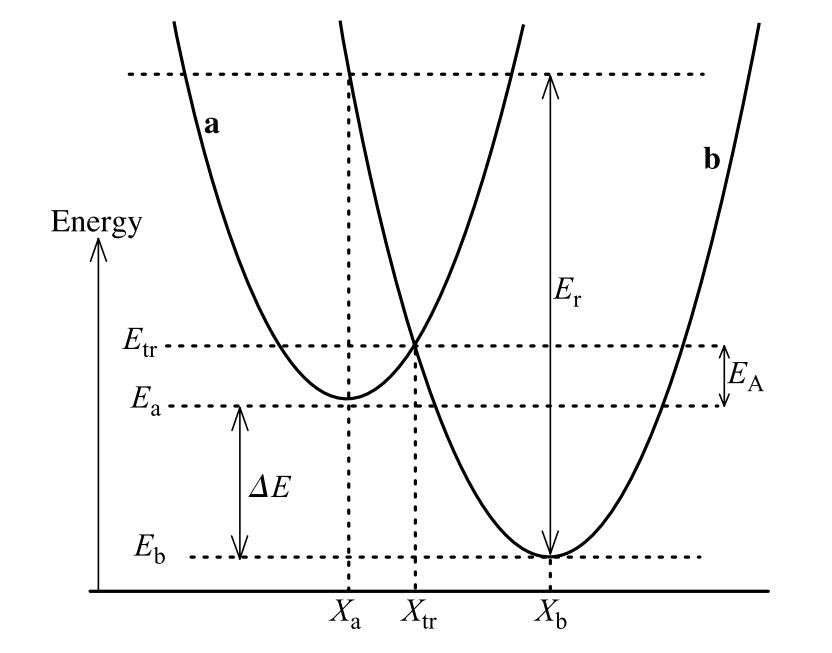
\includegraphics[width=10cm]{fig/Marcus.jpg}
          \caption{\textbf{Marcus理论的模型图}}
          \label{Marcus figure}
        \end{figure}

        在这样的近似下,我们就能画出一个类似于Figure \ref{Marcus figure}的模型图(原则上,图中的能量其实是自由能),根据平移谐振子近似,我们可以写出两个透热态势能面的能量
        \begin{equation*}
          Y_{a}=E_{a}+\frac{K}{2}\left(X-X_{a}\right)^{2}, Y_{b}=E_{b}+\frac{K}{2}\left(X-X_{b}\right)^{2}
        \end{equation*}
        在这里我们定义重整能(Reorganization Energy):电子从第一个势能面底垂直跃迁到第二个势能面上之后,从这个位置驰豫到第二个势能面的基态需要的能量,即图中的$E_r$\footnote{不同地方定义略有区别,但是为了推出这个公式,都是等价的}。那么重整能的大小也很容易计算
        \begin{equation*}
          E_{r}=Y_{2}\left(X_{a}\right)-Y_{2}\left(X_{b}\right)=E_{b}+\frac{K}{2}\left(X_{a}-X_{b}\right)^{2}-E_{b}=\frac{K}{2}\left(X_{a}-X_{b}\right)^{2}
        \end{equation*}
        可以看到,图中两个势能面有一个交叉,我们就认为这个交叉点就是从a态到b态过程的过渡态,那么过渡态对应的反应坐标为
        \begin{equation*}
          \begin{array}{c}{Y_{a}\left(X_{\mathrm{tr}}\right)=Y_{b}\left(X_{\mathrm{tr}}\right)} \\ {E_{a}+\frac{K}{2}\left(X_{\mathrm{tr}}-X_{a}\right)^{2}=E_{b}+\frac{K}{2}\left(X_{\mathrm{tr}}-X_{b}\right)^{2}} \\ {E_{a}+\frac{K}{2}\left(X^{2}-2 X_{a} X+X_{a}^{2}\right)=E_{b}+\frac{K}{2}\left(X^{2}-2 X_{b} X+X_{b}^{2}\right)} \\ {X_{\mathrm{tr}}=\frac{E_{a}-E_{b}+\frac{K}{2}\left(X_{a}^{2}-X_{b}^{2}\right)}{K\left(X_{a}-X_{b}\right)}}\end{array}
        \end{equation*}
        过渡态对应的能量为
        \begin{equation*}
          \begin{array}{l}{E\left(X_{\mathrm{tr}}\right)=E_{a}+\frac{K}{2}\left(X_{\mathrm{tr}}-X_{a}\right)^{2}} \\ {=E_{a}+\frac{K}{2} \frac{\left[E_{a}-E_{b}+\frac{K}{2}\left(X_{a}^{2}-X_{b}^{2}\right)-K X_{a}^{2}+K X_{a} X_{b}\right]^{2}}{K^{2}\left(X_{a}-X_{b}\right)^{2}}} \\ {=E_{a}+\frac{K}{2} \frac{\left[E_{a}-E_{b}-K\left(X_{a}-X_{b}\right)^{2} / 2\right]^{2}}{K^{2}\left(X_{a}-X_{b}\right)^{2}}} \\ {\therefore E_{A}=\frac{K}{2} \frac{\left[E_{a}-E_{b}-K\left(X_{a}-X_{b}\right)^{2} / 2\right]^{2}}{K^{2}\left(X_{a}-X_{b}\right)^{2}}=\frac{\left(\Delta E+E_{r}\right)^{2}}{4 E_{r}}}\end{array}
        \end{equation*}
        最后得到的$E_A=E\left(X_{\mathrm{tr}}\right)-E_a$是从a态到b态的活化能,$\Delta = E_b-E_a$是反应的反应能变,根据过渡态理论我们得到
        \begin{equation*}
          k_{r a t e}=A e^{-\frac{E_{A}}{k T}}=A e^{-\frac{\left(\Delta E+E_{r}\right)^{2}}{4 k T E_{r}}}
        \end{equation*}
        这就是Marcus理论的雏形,也是Marcus提出的函数形式,这个指前因子$A$,在透热极限下,是可以通过微扰法来计算推导的,最后的结果是
        \begin{equation}
          k=\frac{V^{2}}{\hbar} \sqrt{\frac{\pi}{\lambda k_{\mathrm{B}} T}} \exp \left(-\frac{\left(\lambda+\Delta G^{0}\right)^{2}}{4 \lambda k_{\mathrm{B}} T}\right)
          \label{Marcus theory}
        \end{equation}
        在式(\ref{Marcus theory})中,$V$代表了透热表象下两个态的相互作用(哈密顿量非对角元),我们按照通用的习惯,将重整能记为$\lambda$,反应的能量变化改为吉布斯自由能变。

        与经典过渡态理论告诉人们的一样,一个态到另一个态的转化,并不是能量下降越多速度越快的,Marcus理论的一个重要结论在于,当一开始$\Delta G^{0}$较大时,转化较慢,随着$\Delta G^{0}$减小,转化速度逐渐加快,这个速度的最大值,就是当$\Delta G^{0} = -\Lambda$时,在这之后,如果继续降低第二个态的能量,这个转化速度反而会下降。$\Delta G^{0}< -\lambda$的区域,通常称为Marcus反转区。

        但是过渡态理论和Marcus理论并非这么简单就结束了,它隐含着丰富的内涵。我们知道电子的运动速度是远快于原子核的,这也是BO近似的来源。在跃迁的理论中,我们会有被称为Franck-Condon原理的理论:电子的跃迁是垂直跃迁,即在势能面上,电子跃迁的瞬间原子核的位置(反应坐标)是不变的。那么问题来了,当体系处于光辐射下,电子跃迁的能量差是由外界辐射能量提供的,但是对没有外界辐射时,电子的能量是由热能,即原子核振动的能量提供的,因此实际上电子跃迁只发生在了两个态上相互作用最大,通常是能量最近的能级(电子能级加核振动能级)附近,所以电子态的跃迁问题其实是一个电子-声子(核振动)耦合的问题。Marcus理论对这个过程中的电-声子耦合的作用浓缩在了一个重整能里,这样的描述显然是充分的。
      \section{势间跳跃方法与FSSH}
        势间跳跃 (Surface Hopping)方法是一种混合量子经典(Mixed-Quantum-Classical)方法\footnote{需要注意混合量子经典与半经典方法(Semi-Classical)不同,前者一般指方法中既有经典部分又有量子部分,后者偏向量子力学做经典近似,演化一个半量子半经典的方程},它是非绝热动力学中非常常用的一类,尽管很早就有类似的思路,直到1990年John Tully提出了最少跃迁的势间跳跃(Fewest Switches Surface Hopping, FSSH)方法\cite{Tully1990},在这之后surface hopping方法被大量使用并且一直被发展,王老师课题组的核心研究方向就是SH方法中某些复杂问题的处理以及将其往更大体系更多自由度推广。

        在势间跳跃方法,原子核做经典处理,按照分子动力学的方法运动,但是其感受到的势能是由电子势能而非力场提供,电子的势能是根据电子的Schr\"odinger方程描述的,即电子的运动是量子处理。简单地说,如果读者熟悉分子动力学,那么这套方法理解起来是非常容易的,它的思路非常平凡,即在一个某一个时刻开始,在$dt$的时间间隔内用经典方法演化核的运动,然后计算电子波函数在这个$dt$内的演化,电子势能梯度为原子核的运动提供力,进而演化下一个时刻的原子核运动和电子运动,如此重复,就可以得到非绝热动力学的模拟结果。

        当然尽管图像上非常简单,但是实际操作起来会有各种各样的问题,比如下一小节中稍微涉及的势能面交叉和退相干的问题,包括电子如何在势能面上运动,都是现在仍然在讨论的重要问题,我们都会稍作涉及,但是首先要回到最早的FSSH方法上来。

        之所以称为Surface Hopping,就是因为在这套方法中电子的运动其实是在势能面间的跳跃,在特定的时刻内,电子只会存在于其中的某一个势能面(即通常说的active态),不同的SH方法的核心区别通常在于如何定义电子在不同势能面之间的跃迁概率,什么时候会跃迁。当然如果我们研究一个简单的隧穿问题,单一的SH计算只会得到一个固定的结果,要么穿过了势垒要么被反射等等,不会得到具体的隧穿概率数据,因此SH方法通常需要做很多次轨迹,然后取轨迹平均来得到物理观测量的结果。

        在等式(\ref{time-depend-coeff})中,我们演化波函数的系数,但是为了方便,我们会使用密度矩阵的演化,在等式(\ref{linear combination})的展开形式下,密度矩阵的矩阵元定义为$a_{kj}=c_k c_j^*$,在这个两边取时间导数并将(\ref{time-depend-coeff})的结果代入,我们就得到了关键性的等式
        \begin{equation}
          \begin{aligned} i \hbar \dot{a}_{k j}=& \sum_{T}\left\{a_{l j}\left[V_{k l}-i \hbar \dot{\mathbf{R}} \cdot \mathbf{d}_{k l}\right]\right.\\ &-a_{k l}\left[V_{l j}-i \hbar \dot{\mathbf{R}} \cdot \mathbf{d}_{i j}\right] \} \end{aligned}
          \label{time-de DM}
        \end{equation}
        我们通常关心的是密度矩阵的对角元,就是总电子波函数在某个势能面上的\textbf{布居}(\textbf{Population}),令上式中的$k=j$我们得到
        \begin{equation}
          \dot{a}_{k k}=\sum_{l \neq k} b_{k l}
        \end{equation}
        其中
        \begin{equation}
          b_{k l}=2 \hbar^{-1} \operatorname{Im}\left(a_{k l}^{*} V_{k l}\right)-2 \operatorname{Re}\left(a_{k l}^{*} \dot{\mathbf{R}} \cdot \mathbf{d}_{k l}\right)
          \label{time-de DM diagnol}
        \end{equation}
        而$\dot{a}_{k k}$就是势能面$k$上的布居变化,这里我们引入最少跳跃(Fewest Switches, FS)的思想,即在一个时间间隔$\mathrm{d}t$内的布居变化完全由当前态向其他态的跃迁提供,以两个态的体系为例,如果在时间$t$时,假设所有轨迹中电子当前处在1态的轨迹数为$N_1(t)=a_{11}(t)N$,其中$a_{11}$是$t$时刻电子在1态的布居,$N$为总轨迹数。与之类似,我们有$t$时刻处于2态的轨迹数$N_2(t)=a_{22}(t)N$,在很小的时间间隔$\mathrm{d}t$之后,两个布居为$a_{11}(t+\mathrm{d}t)$和$a_{22}(t+\mathrm{d}t)$,不失一般性,我们假设$a_{11}(t)<a_{11}(t+\mathrm{d}t),a_{22}(t)>a_{22}(t+\mathrm{d}t)$,我们就固定这个时间间隔内从态1跃迁到态2的轨迹数为$a_{11}(t+\mathrm{d}t)-a_{11}(t)$,而从态2跃迁到态1的轨迹数为$0$,原则上可以两者各加一个常数,FS的思想等价于固定这个常数为$0$。这样处理之后,我们得到$\dot{a}_{22}=-\dot{a}_{11}=\frac{a_{11}(t)-a_{11}(t+\mathrm{d}t)}{\mathrm{d}t}$,则如下定义的跃迁概率
        \begin{equation}
          P_{1\rightarrow2}\equiv\frac{a_{11}(t)-a_{11}(t+\mathrm{d}t)}{a_{11}(t)}=\frac{\dot{a}_{22} \mathrm{d}t }{ a_{11}(t)}
        \end{equation}
        如果只有两个能级,将等式(\ref{time-de DM diagnol})代入得到
        \begin{equation}
          P_{1\rightarrow2}=\frac{b_{21} \mathrm{d}t }{ a_{11}(t)}
          \label{hopping probability}
        \end{equation}
        上式就是FSSH的核心公式\footnote{细心的读者可能会发现与Tully原文中的分母不完全相同,但是本文的推导更加合理一点,通常也是使用这一套公式,当然,由于$\mathbf{d}t$内密度矩阵几乎不会变化,究竟是用$t$时刻还是$t+\mathbf{d}t$时刻对结果的影响不大。}。FSSH单个轨迹的流程就是先初始化,赋予研究的体系一个初始动能(动量)和位置,然后每个$\mathbf{d}t$内先用经典力学的方法演化原子核的运动,再利用等式(\ref{hopping probability})计算出当前态跃迁到其他态的概率,用随机数的方法判断是否跃迁,同时还要判断跃迁之后是否满足能量守恒,如果满足,则完成跃迁并修正体系原子核运动的速度,不断重复上述过程就得到了动力学演化的结果。
        
      \section{鸟瞰SH方法中的特殊问题}
        本小节将会简要地介绍在SH发展这么多年来,出现的很多问题,包括王老师组学长学姐在这方面的工作的简介,但是由于编者水平有限,只能略作介绍,并且有很大概率在细节上理解不全面甚至有错误,而王老师课题组的各位学长学姐在这方面有更多可说的内容。

        \paragraph{Trivial Crossing:}在势能面上演化动力学的过程中,势能面通常会有各类的交叉和相互作用,多数可以归为Trivial Crossing或者Avoided Crossing,两者的定义Figure \ref{two kinds of crossing}所示
        \begin{figure}
          \centering
          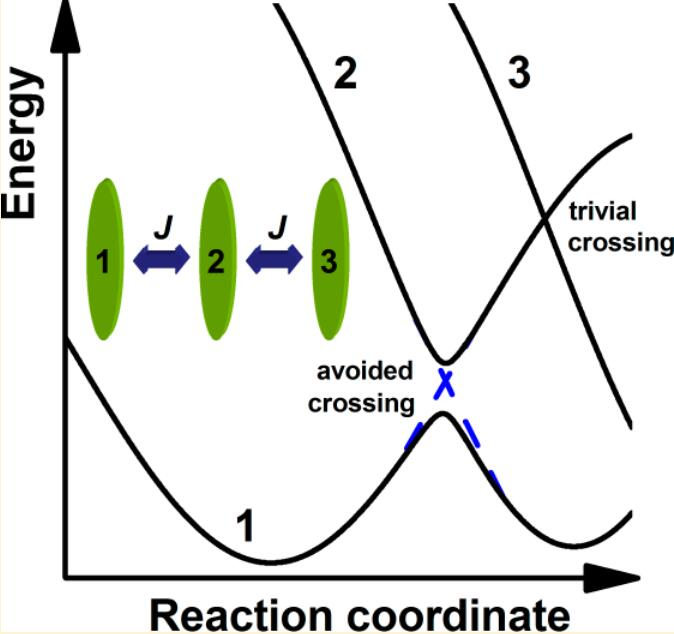
\includegraphics[width = 8cm]{fig/crossing.jpg}
          \caption{\textbf{SH两种Crossing的定义}}
          \label{two kinds of crossing}
        \end{figure}
        图中表示分子1和2之间有相互作用,当它们的势能面交叉时就会产生Avoided Crossing,1和3之间由于距离较远没有相互作用,但是在能量空间下,它们对应的态可能十分接近,这样使得它们的势能面存在交叉,即为Trivial Crossing。另外,Trival Crossing并非只存在于实空间距离很远的两个分子上,即使在同一个分子中,由于轨道之间没有或者相互作用非常小(比如对称性不同的分子轨道,$\sigma$键和$\pi$键之间)但是能量接近,也是可能发生Trivial Crossing的。

        但是由于电子结构计算是按照能量排序的,所以在发生Trivial Crossing的地方会有能级顺序的错误,误将别处毫不相关的能级作为了当前能级,而且根据等式(\ref{analytical dij}),此处的NAC是无法被描述的,通常会由于数值计算时过大而使得跃迁概率接近1,发生不该发生的跃迁,比如从分子1直接跳到分子3。

        为了处理这类问题,王老师发展了很多相关方法,这也是王老师前几年工作的重心。比如SC-FSS和CC-FSSH,后者把常见的Trivial Crossing进行了分类,每一类都有对应的解决方案,基本已经可以处理此类问题,具体内容可以参阅相关文章\cite{wang2014simple}\cite{Qiu2018}\cite{Bai2018}。

        \paragraph{超交换问题:}我们继续用上文中的图,同时联想化学里的过渡态理论,如果只有1态和2态之间、2态和3态之间有相互作用,但是1态和3态之间没有,按照SH方法的处理,如果想从1态到3态必须经过2态,但如果此时2态有较高的能量,高于此时原子核运动的动能,如果跃迁发生,就不满足能量守恒,尽管1态和3态之间的势能差可以被原子核动能满足,由于SH的操作方法,系统是不可能从1态到达3态的。但这并非真实情况,在量子力学中存在隧穿行为,因此实际上体系是会从1态到达3态的,SH这个错误的来源是忽略了原子核的量子效应导致的。当然,这不意味着SH不能处理超交换问题,王老师提出了在Liouville空间下Surface Hopping\cite{wang2015fewest},可以很好地处理超交换和隧穿的问题。

        \paragraph{退相干:}Surface Hopping方法中最大的短板之一就是被称为“过相干(over-coherence)”的现象。为了介绍这种现象,我们先回忆一下FSSH,我们利用运动方程来演化经典的原子核运动和量子的电子演化,这里其实存在一个问题,即使电子的状态和核受力是预先对应好的,但是两者运动的自洽性仍然难以保证。全量子的方法可以保证这个自洽性的存在,SH对原子核的经典处理是过相干现象的缘由。

        在一个单一的轨迹中,不同电子态的电子的运动是一直耦合在一起的,如果在某些情况下,原子核在两个势能面上的受力相差较大,甚至反向,在真实的全量子演化下,两个势能面上的原子核的波包将会分离,这也将导致电子波函数分离成两个部分,不再耦合在一起,然而原始的FSSH方法是无法处理这种退相干(decoherence\footnote{在王老师课题组的文章中有时称为Branching Correction, BC})现象的。因此正确的退相干策略也是SH方法发展的重要主题。
        
        \paragraph{相位修正:}传统的FSSH方法在处理不同势能面的波函数时会有一个相位差的问题。这个问题的来源是当FSSH决定电子要跃迁时,电子是直接跃迁到当前原子核结构下的其他势能面。但是由于势能面的能量不同,其对应的原子核速度不同,以两能级系统举例,如果两个原子核波包同时开始演化,电子一开始位于基态势能面,能量较高的势能面原子核速度较低(这是能量守恒的要求),因此在电子跃迁时,相同相位对应的激发态还未运动到基态波函数对应的位置,而是在其之前,这要求实际操作电子跃迁时,需要对波函数的相位进行修正(Phase Correction)。

    \chapter{全局优化问题}
      全局优化问题其实是个数学问题,简单地说就是有一个复杂的高维函数,我们如何求得其最小值的问题,但是这个数学问题在化学物理等领域都有重要的意义,我们也主要是全局优化算法在我们的问题中的应用。以最常见的也是王老师课题组之前处理的一个例子,如果任意两个原子之间的相互作用势能是LJ势,给定两个原子,可以通过对坐标求导等于0的方式找到这两个原子的最稳定的位置,但是如果是三个原子,事情就会变得麻烦起来,那如果是一千个原子呢?这个问题其实等价于一个三千维的函数的最小值问题,想通过简单的解析方法求解是几乎不可能的。即使人们有强大的计算机,这样的一个问题还是不简单的,尤其是自由度增多时额外增加的计算量更是不可估计的。人们基于各种各样的思路发展了一系列全局优化算法,限于编者水平,在这里我们只能简单介绍其中的几种。

      我们就以分子原子团簇的优化举例子,我们希望优化的函数是体系总能量。我们先介绍一种最简单的思路,那就是梯度下降,即使是高维函数,你总是可以通过数值的方法求解这一点上能量关于某个自由度的导数(梯度),然后沿着负导数的方向移动,直到达到导数为0为止。这相当于沿着受力的方向一路运动直到达到一个极小值,这种方法的问题也是显然的,就是我们只能达到极小值而非最小值,当自由度非常多时,体系的极小值点可能非常之多,我们一般称这种方法为局部优化,譬如高斯等软件计算分子的最优构型时就是用的类似的思路(当然不是类似LJ势的分子力场的势能,而是量子化学计算的势能)。

      为了尽可能找到极小值,我们需要尽可能搜查整个势能面(直接遍历的计算量是巨大的,但是小体系少自由度情况也可以做),这意味着我们有时需要反着能量下降的方向运动进而跨过一些势垒区域,但是我们又不需要跨越太大的无意义的势垒,解决这个问题就是利用Monte Carlo模拟中接受分子构型的类似方法,认为有一个所谓的温度存在,即不是能量最低原理,而是满足某种分布。在全局优化问题里,我们不一定采用玻尔兹曼分布型的函数,原则上为了达成目的的任何函数形式都可以。当体系沿着某一个自由度能量升高时,用这个函数来判断是否接受构型。

      上面两个思路是全局优化方法的基础,我们通常是多种思路混合得到最后的算法。正如刚刚说的,全局优化算法里可以用遍历的方法寻找最小值,这是最简单粗暴计算量最大的,另一个极端就是完全取随机构型,然后比较取到的随机构型的能量然后从中选中最小的。显然这两种方法都不是特别靠谱,接下来我们介绍一种常用的也是王老师组处理LJ团簇的方法:\textbf{Basin Hopping}。简单的说,这是一种与MC模拟相类似的方法,核心思路为我先有一个初始的分子构型,然后对其进行局部优化得到一个局部优化的结构和对应的能量。然后在这个构型上每个自由度随机移动一点,从这个随机移动得到的构型再做局部优化,如此反复,直到有足够多的极小值,从中挑出最小的那个。这个方法十分简单有效,其随机移动的思路与MC模拟相仿,甚至目的都是一样的:跨过一些势垒尽可能遍历相空间。而王老师课题组还在这里面加入了很多很多为了节省计算量的功能,具体细节只有仔细看过代码才能理解。但是其中非常关键的一部分就是把绝大多数的优化在离散空间内完成,这样原子间的能量就不用每次都计算,而是把离散空间每个格点距离的能量提前算好保存在一个数组里,以后每次使用时只需要调用数组元素就行了。

      全局优化算法中有一类比较出名的叫做模拟\textbf{退火算法}(Simulate Anneal)。模拟退火是模拟材料合成中的退火步骤,对于分子的能量优化这个问题,在这个系统中有一个温度的概念,这个温度某种程度上相对应着体系的动能。这个算法的核心思路是先升温,使得体系拥有一个较高的动能,这样它在随机变化过程中就可以克服很高的势垒,进而有可能遍历势能面上尽可能多的位置,然后降温(退火),原本在势能面不同位置的分子动能逐渐减小,他们的运动进而无法跨越势垒,就落到了势能面上的某个极小值位置。如果升温时随机运动的范围已经能遍历了整个势能面,那么在最后所有极小值处寻找分子的结构,就能得到体系的最小值。

      另一类比较火爆的思路就是\textbf{遗传算法},这是一个借鉴生物遗传进化的非常有趣的算法。我们首先把分子的结构量化定义为一系列变量,称之为基因,最初,生成一系列随机的结构,称为亲代,然后定义一种“进化”,即用他们的能量函数来表征他们的生存优势,经过一次次筛选,只有能量更低的(生存优势更大)的分子会留下。然后这些有优势的分子进行“杂交”,将他们的结构按某种方法进行组合生成新的子代分子,子代的分子之间再按照某种方式进行筛选,留下能量更低的分子,再进行“杂交”,如此反复,最后就能得到能量较低的“进化”之后的分子。

      向生物学习也是全局优化中的常见思路,除了遗传算法之外,现在还有基于蚂蚁寻找食物思路的算法等,不予详细介绍。另外,可以看出,机器学习在这方面也肯定有一定的建树,但是势能面通常过于复杂,简单的机器学习网络可能无法实现。

      当然,全局优化的问题远远不限于分子能量优化上,包括求条件极值,减小误差,拟合等多种问题都可以使用全局优化的思路进行处理,有时候往往能产生有趣的效果。\sout{初一看只有一两个做全局优化的学长学姐,做到最后就会发现,组内一大半的人都在做全局优化}

      \chapter{相空间-量子哈密顿动力学(PS-QHD)}
      \begin{enumerate}
  \item 在更多的化学问题中,电子会发生跃迁,Born-Oppenheimer近似失效,比如光催化反应,光电材料中的电荷传输,无辐射跃迁,生命活动中的光合作用,呼吸作用等,必须使用更普适的非绝热动力学研究。

  \item 非绝热动力学的思想分为两派:追求严格,将电子与原子核做量子化处理;追求效率,将原子核作经典处理。需要在拥有量子效应的基础上保证计算效率。David Manolopoulos 提出的环聚合物方法(ring polimer)是一种可能,并已被John Tully和Frank Huo等人与面间跳跃方法相结合。而该方法只能处理热力学平衡态,但很多化学过程发生在非平衡态。Oleg Prezhdo提出的量子哈密顿动力学(QHD)是另一种可能。

  \item QHD从经典描述出发,逐级添加量子效应修正,添加无穷阶修正即可达到全量子严格解。

  \item QHD用Hilbert空间描述,以一系列算符的期望值作为变量组来描述粒子的运动过程。由于经典力学中确定粒子的运动状态只需要坐标和动量,因此HS-QHD的一阶变量直接对应于经典力学,而高阶变量选择坐标算符和动量算符高阶数的乘积。由于坐标算符和动量算符的不对易,它们的乘积并非Hermite算符,而只有Hermite算符的期望值才是实验可观察的实数值,因此Weyl对称化被引入来保证变量组纯实。

  \item Hilbert空间中任意算符$\hat{A}$期望值随时间的演化遵循Ehrenfest定理:
  \begin{equation}
  \frac{d}{dt}\mean{\hat{A}}=\mean{\frac{\partial}{\partial t} \hat{A}}+\mean{\frac{1}{i\hbar}\left[\hat{A},\hat{H}\right]}
  \end{equation}

  \item HS-QHD的演化方程具有级联方程组形式,即低阶量的含时演化依赖于高阶量的值。我们计算的动力学只能采用有限阶,为使方程组完备只能在计算的有限阶的基础上去近似表达未知的高阶量,从而完成方程组截断,求得参数,通行的近似方法是将高阶中心矩近似为各种可能的低阶中心矩在保持变量的总数及总阶数不变时乘积的叠加,以三阶和四阶为例:
  \begin{align*}
  &\mean{(\hat{A}-\mean{\hat{A}})(\hat{B}-\mean{\hat{B}})(\hat{C}-\mean{\hat{C}})}\\
  \sim & \sum_{\text{轮换求和}}\mean{(\hat{A}-\mean{\hat{A}})(\hat{B}-\mean{\hat{B}})}\mean{(\hat{C}-\mean{\hat{C}})}\\
  =& 0
  \end{align*}
  \begin{align*}
  &\mean{(\hat{A}-\mean{\hat{A}})(\hat{B}-\mean{\hat{B}})(\hat{C}-\mean{\hat{C}})(\hat{D}-\mean{\hat{D}})}\\
  \sim & \sum_{\text{轮换求和}}\mean{(\hat{A}-\mean{\hat{A}})(\hat{B}-\mean{\hat{B}})}\mean{(\hat{C}-\mean{\hat{C}})(\hat{D}-\mean{\hat{D}})}
  \end{align*}\footnote{最后求和展开每一个系数为1,虽然这看起来有点奇怪。}

  问题:
  \begin{enumerate}

    \item 算符乘法不可交换,存在算子序
    \item 近似只对中心矩有效,需要转换回变量组,而变量组是对称化的原点矩,导致这一转换复杂冗长,难以卸除通用公式

    \item 不显式地保证高阶收敛性,即不保证睡着中心矩阶数的上升截断误差不断减小直至在无穷阶极限收敛到零。

  \end{enumerate}


  \item 量子力学等价表述形式:
  \begin{itemize}
    \item Hilbert 空间及其关联的波函数、密度矩阵和力学量算符
    \item 相空间及其关联的Wigner分布函数和力学量函数
  \end{itemize}

  \item 相空间表象在研究混合量子经典问题更有优势,在$\hbar \rightarrow 0$的经典极限可直接转换到经典相空间,在$\hbar$越来越重要时量子效应项按照依赖$\hbar$的阶数逐渐发挥作用,符合从经典向量子过度并按精度选择合适描述的思想。自然保证变量组纯实,因为Wigner函数和力学函数都是实函数,故坐标函数和动量函数的乘积仍为实函数,期望值为实数。

  \item 高阶变量除去对应阶的标准差来避免由分布宽度引起的不必要数字膨胀,采用
  \begin{equation}
    \mean{\frac{1}{m!n!}\left(\frac{x-\mean{x}}{\sigma_x}\right)^m\left(\frac{p-\mean{p}}{\sigma_p}\right)^n}
    \end{equation}

  \item 相空间乘法可交换,在采用通行的级联方程组截断方案时将不会遇到算子序问题。由于变量组采用相空间无量纲中心矩,不存在转换回原点矩及对称化问题,对不同变量有共通形式。无穷阶收敛性问题则仍然存在,在采用合适的截断方案后才能得到解决。  
\end{enumerate}
\section{相空间Ehrenfest定理}
\begin{enumerate}
  \item 相空间Ehrenfest定理:
  \begin{equation}
  \frac{d}{dt}\mean{A}=\mean{\frac{\partial}{\partial t} A}+\mean{\left\{\{A,H\}\right\}}
  =\mean{\frac{\partial}{\partial t} A}+\mean{\left\{\{A,\frac{p^2}{2 m}+V\}\right\}}
  \end{equation}

  \item $\{\{*,*\}\}$为Moyal括号,定义为
  \begin{align}
  \{\{A,H\}\}&\equiv \frac{2}{\hbar}A \sin \left[\frac{\hbar}{2} (\overleftarrow{\partial_x}\overrightarrow{\partial_p}-\overleftarrow{\partial_p}\overrightarrow{\partial_x})\right]H\\
  &=\{A,H\}+\sum^\infty_{j=1}\frac{(-1)^j}{(2j+1)!}\left(\frac{\hbar}{2}\right)^{2j}A(\overleftarrow{\partial_x}\overrightarrow{\partial_p}-\overleftarrow{\partial_p}\overrightarrow{\partial_x})^{2j+1} H
  \end{align}
  偏导数符号的左右箭头代表该偏导数向左或向右作用,$\{*,*\}$为Poisson括号。

  \item 将A替换为变量组,得到演化方程,可以看到,前二阶量的演化中不会出现$\hbar$,是纯经典及准经典项:
  \begin{equation}
  \begin{cases}
  \frac{d}{dt}\mean{x}=\frac{1}{m}\mean{p}\\
  \frac{d}{dt}\mean{p}=-\mean{\grad V}\\
  \frac{d}{dt}\sigma_x = \frac{1}{m}\rho \sigma_p\\
  \frac{d}{dt} \rho = \frac{1}{m}\frac{\sigma_p}{\sigma_x} - \frac{1}{\sigma_p} \mean{(\grad V- \mean{\grad V })\left(\frac{x-\mean{x}}{\sigma_x}\right)}-\left(\frac{1}{\sigma_x}\right)\\
  \frac{d}{dt}\sigma_p=- \mean{(\grad V-\mean{\grad V })\left(\frac{p-\mean{p}}{\sigma_p}\right)}
  \end{cases}
  \end{equation}

  高阶项的$\hbar$依赖性与$A$对$p$和$\grad V$对$x$的非零偏导数有关:\footnote{在这里面为了和指数里面的$m$区分使用$M$来代表质量。}
  

\end{enumerate}
\vspace{-0.5cm}
\begin{align*}
  &\frac{d}{dt}\mean{\frac{1}{m!n!}\left(\frac{x-\mean{x}}{\sigma_x}\right)^m\left(\frac{x-\mean{x}}{\sigma_x}\right)^n}\\
  &= \frac{n+1}{M}\frac{\sigma_p}{\sigma_x}\mean{\frac{1}{(m-1)!(n+1)!}\left(\frac{x-\mean{x}}{\sigma_x}\right)^{m-1}\left(\frac{p-\mean{p}}{\sigma_p}\right)^{n+1}}\\
  &\quad -\frac{1}{\sigma_p m!}\mean{\frac{1}{(n-1)!}\left(\frac{x-\mean{x}}{\sigma_x}\right)^{m}\left(\frac{p-\mean{p}}{\sigma_p}\right)^{n-1}(V'-\mean{V'})}\\
  &\quad + \sum_{j=1}^{Floor(\frac{n-1}{2})}\frac{(-1)^{j+1}}{(2j+1)!\sigma_p^{2j+1}}\left(\frac{\hbar}{2}\right)^{2j}\frac{1}{m!}\mean{\frac{1}{[n-(2j+1)]!}\left(\frac{x-\mean{x}}{\sigma_x}\right)^{m}\left(\frac{p-\mean{p}}{\sigma_p}\right)^{n-2j-1}V^{2j+1}}\\
  &\quad - \left(\frac{m}{\sigma_x}\frac{d\sigma_x}{dt}+\frac{n}{\sigma_p}\frac{d\sigma_p}{dt}\right)\mean{\frac{1}{m!n!}\left(\frac{x-\mean{x}}{\sigma_x}\right)^{m}\left(\frac{p-\mean{p}}{\sigma_p}\right)^{n}}
  \end{align*}

\section{相空间分布函数}
\begin{enumerate}
  \item 为实现方程组截断,采用类似变分的手段得到相空间分布函数。原则上,相空间分布函数形式可以有多种选择,这里我们选择与我们的变量组形成线性映射的函数空间:
  \begin{equation}
  P(x,p)=G(x,p)\sum_{0 \leq i+j \leq N} c_{ij} f_{ij} (x,p)
  \end{equation}
  其中$P(x,p)$是相空间分布函数,$G(x,p)$是任意光滑函数,$f_{ij}(x,p)$是任意保证无穷阶完备性的基函数,$N$是我们计算的最高阶PS-QHD变量的阶数,$c_{ij}$是待定参数。待定参数的个数为$1+N(N+3)/2$,与前N阶变量总数加归一化所得的条件个数相同。我们可以通过一个线性方程来求解这些待定参数:
  \begin{align*}
  &\sum_{0\leq i+j\leq N}\left[\frac{1}{k!l!}\int G(x,p)c_{ij}f_{ij}(x,p)\left(\frac{x-\mean{x}}{\sigma_x}\right)^{k}\left(\frac{p-\mean{p}}{\sigma_p}\right)^{l}\,dxdp\right]\\
  &=\mean{\frac{1}{k!l!}\left(\frac{x-\mean{x}}{\sigma_x}\right)^{k}\left(\frac{p-\mean{p}}{\sigma_p}\right)^{l}}
  \end{align*}

  而后
  \begin{equation}
  \mean{A}=\int A(x,p) P(x,p) \, dxdp
  \end{equation}

  如果$G(x,p)$为高斯函数而$f_{ij}(x,p)$为Hermite多项式,其低阶运动方程与通行的HS-QHD近似截断方法一致:
  \begin{equation}
  \begin{cases}
  G(x,p)=\frac{1}{2\pi \sigma_x\sigma_p\sqrt{1-\rho^2}}e^{-\frac{1}{2(1-\rho^2)}\left[\left(\frac{x-\mean{x}}{\sigma_x}\right)^2-2\rho\left(\frac{x-\mean{x}}{\sigma_x}\right)\left(\frac{p-\mean{p}}{\sigma_p}\right)+\left(\frac{p-\mean{p}}{\sigma_p}\right)^2\right]}\\
  \sum_{0\leq i+j \leq N}c_{ij}f_{ij}(x,p)=\sum_{0\leq i+j \leq N}\frac{c_{ij}}{i!j!}\left(\frac{x-\mean{x}}{\sigma_x}\right)^{k}\left(\frac{p-\mean{p}}{\sigma_p}\right)^{l}
  \end{cases}
  \end{equation}
\end{enumerate}




      \bibliographystyle{unsrt}
      \bibliography{reference}


  \end{document} 

